% !TEX encoding = IsoLatin

% La riga soprastante serve per configurare gli editor TeXShop, TeXWorks
% e TeXstudio per gestire questo file con la codifica IsoLatin o Latin 1
% o ISO 8859-1.

% per commentare una riga mettere % al suo inizio
% per s-commentare una riga (ossia attivarla) togliere il % al suo inizio
%
\documentclass[pdfa% formato PDF/A, obbligatorio per l'archiviazione delle tesi di Polito
,cucitura%lascia margine per la rilegatura
%,twoside% per stampa fronte-retro (fortemente consigliato per tesi voluminose, opzionale per le altre)
%,12pt% font pi� grande (12pt) rispetto a quello normalmente usato (11pt)
]{toptesi}
%
\usepackage{hyperref}
\hypersetup{%
    pdfpagemode={UseOutlines},
    bookmarksopen,
    pdfstartview={FitH},
    colorlinks,
    linkcolor={blue},
    citecolor={red},
    urlcolor={blue}
  }
% \documentclass[11pt,twoside,oldstyle,autoretitolo,classica,greek]{toptesi}
% \usepackage[or]{teubner}
%%%%%%%%%%%%%%%%%%%%%%%%%%%%%%%%%%%%%%%%%%%%%%%%%%%%
%
% Esempio di composizione di tesi di laurea.
%
% Questo esempio e' stato preparato inizialmente 13-marzo-1989
% e poi e' stato modificato via via che TOPtesi andava
% arricchendosi di altre possibilita'.
%
% Nel seguito laurea "quinquennale" sta anche per "specialistica" o "magistrale"

% Cambiare encoding a piacere; oppure non caricare nessun encoding se si usano
% solo caratteri a 7 bit (ASCII) nei file d'entrata.
%
\usepackage[latin1]{inputenc}% IMPORTANTE! usare codifica ISO-8859-1 per le lettere accentate

% temporaneo
\usepackage[dvipsnames]{xcolor}

\usepackage{amssymb}
\usepackage{amsmath}
\usepackage{algorithm}
\usepackage{algpseudocode}
\usepackage{graphicx}
\usepackage{xcolor}

% !TEX encoding = IsoLatin

% per inserire uno spazio "fantasma" nella definizione di un'abbreviazione
\usepackage{xspace}

% per inserire un DOI senza problemi coi caratteri "strani" ivi presenti
\usepackage{doi}
\renewcommand{\doitext}{DOI }% originally was "doi:"

% per inserire correttamente le unit� di misura SI (incluse quelle binarie)
\usepackage[binary-units]{siunitx}
% se si desidera usare / invece che la potenza -1 per indicare "al secondo"
\sisetup{per-mode=symbol}

% per inserire codice di programmazione complesso
\usepackage{listings}% per inserire codice di programmazione complesso
\lstset{
basicstyle=\ttfamily,
columns=fullflexible,
xleftmargin=3ex,
breaklines,
breakatwhitespace,
escapechar=`
}

% modify some page parameters
\setlength{\parskip}{\medskipamount}

% riga orizzontale
\newcommand{\HRule}{\rule{\linewidth}{0.2mm}}
% esempio di creazione di semplici abbreviazioni
\newcommand{\ltx}{\LaTeX\xspace}
\newcommand{\txw}{TeXworks\xspace}
\newcommand{\mik}{MikTex\xspace}
\newcommand{\html}{HTML\xspace}
\newcommand{\xhtml}{XHTML\xspace}

% esempio di creazione di un'abbreviazione con un parametro (il cui uso � indicato da #1)
\newcommand{\cmd}[1]{\texttt{#1}\xspace}
% per citare un RFC, es. \rfc{822}
\newcommand{\rfc}[1]{RFC-#1\xspace}
% per citare un file (es. \file{autoexec.bat}) o una URI fittizia (es. \file{http://www.lioy.it/})
% per le URI vere usare \url o \href
\newcommand{\file}[1]{\texttt{#1}\xspace}
% per inserire codice di esempio in-line
\newcommand{\code}[1]{\lstinline|#1|}
% importante per i pathname Windows perch� non si pu� usare \ essendo un carattere riservato di Latex
\newcommand{\bs}{\textbackslash}
% definizione di un termine: formattazione ed inserimento nell'indice
\newcommand{\tdef}[1]{\textit{#1}\index{#1}}
% meta-termine, usato tipicamente nelle definizioni dei tag
\newcommand{\meta}[1]{\textit{#1}}
% abbreviazioni in inglese
\newcommand{\ie}{i.e.\xspace}
\newcommand{\eg}{e.g.\xspace}

\definecolor{codegreen}{rgb}{0,0.6,0}
\definecolor{codegray}{rgb}{0.5,0.5,0.5}
\definecolor{codepurple}{rgb}{0.58,0,0.82}
\definecolor{backcolour}{rgb}{0.95,0.95,0.92}

\lstdefinestyle{mystyle}{
	backgroundcolor=\color{backcolour},   
	commentstyle=\color{codegreen},
	keywordstyle=\color{blue},
	numberstyle=\tiny\color{codegray},
	stringstyle=\color{codepurple},
	basicstyle=\ttfamily\footnotesize,
	breakatwhitespace=false,         
	breaklines=true,                 
	captionpos=b,                    
	keepspaces=true,                 
	numbers=left,                    
	numbersep=5pt,                  
	showspaces=false,                
	showstringspaces=false,
	showtabs=false,                  
	tabsize=2
}

\lstdefinelanguage{YARA}{
	morekeywords=[1]{rule, meta, strings, condition},
	morekeywords=[2]{import, ascii, wide, nocase, and, or, all, at, in, of, fullword},
	keywordstyle=[1]\color{Blue},
	keywordstyle=[2]\color{Red},
	sensitive=false,
	morecomment=[l]{//},
	morecomment=[s]{/*}{*/},
	morestring=[b]",
	morestring=[d]',
}

\algdef{SE}% flags used internally to indicate we're defining a new block statement
[CLASS]% new block type
{Class}% "\Class{name}" will indicate the start of the class declaration
{EndClass}% "\EndClass" ends the block indent
[1]% There is one argument, which is the name of the class
{\textbf{class} \textsc{#1}}% typesetting of the start of a class
{\textbf{end class}}% typesetting the end of the class

\DeclareMathOperator*{\argmax}{arg\,max}
\DeclareMathOperator*{\argmin}{arg\,min}

\begin{document}
	
\selectlanguage{english}

\ateneo{Politecnico di Torino}

%%% scegliere la propria facolt� (solo PRIMA dell'AA 2012-2013)
%
%\facolta[III]{Ingegneria dell'Informazione}
%\facolta[IV]{Organizzazione d'Impresa\\e Ingegneria Gestionale}
%\Materia{Remote sensing}% uso sconsigliato

%\monografia{Gestione informatizzata di un magazzino ricambi}% per la laurea triennale
\titolo{Automatic Malware Signature Generation}% per la laurea quinquennale e il dottorato
%\sottotitolo{Metodo dei satelliti medicei}% NON obbligatorio, per la laurea quinquennale e il dottorato

%%% scegliere il proprio corso
%
%\corsodilaurea{Ingegneria dell'Organizzazione d'Impresa}% per la laurea di primo e secondo livello
%\corsodilaurea{Ingegneria Logistica e della Produzione}% per la laurea di primo e secondo livello
%\corsodilaurea{Ingegneria Gestionale}% per la laurea di primo e secondo livello
\corsodilaurea{Ingegneria Informatica}% per la laurea di primo e secondo livello
%\corsodidottorato{Meccanica}% per il dottorato

\candidato{Michele \textsc{Crepaldi}}% per tutti i percorsi
%\secondocandidato{Evangelista \textsc{Torricelli}}% per la laurea magistrale solamente
%\direttore{prof. Albert Einstein}% per il dottorato
%\coordinatore{prof. Albert Einstein}% per il dottorato
\relatore{prof.\ Antonio Lioy}% per la laurea e il dottorato
\secondorelatore{ing.~Andrea Atzeni}% per la laurea magistrale
%\terzorelatore{{\tabular{@{}l}dott.\ Neil Armstrong\\prof. Maria Rossi\endtabular}}% per la laurea magistrale
%\tutore{ing.~Andrea Atzeni}% per il dottorato
%\tutoreaziendale{dott.\ ing.\ Giovanni Giacosa} % solo per la laurea di secondo livello con tesi svolta in azienda
%\NomeTutoreAziendale{Supervisore aziendale\\Centro Ricerche FIAT}
%\sedutadilaurea{Agosto 1615}% per la laurea quinquennale
%\esamedidottorato{Novembre 1610}% per il dottorato
%\sedutadilaurea{\textsc{Novembre} 2017}% per la laurea triennale
\sedutadilaurea{\textsc{Anno~accademico} 2020-2021}% per la laurea magistrale
%\annoaccademico{1615-1616}% solo con l'opzione classica
%\annoaccademico{2006-2007}% idem
%\ciclodidottorato{XV}% per il dottorato
\logosede{logopolito}
%
%\chapterbib %solo per vedere che cosa succede; e' preferibile comporre una sola bibliografia
%\AdvisorName{Supervisors}
%\newtheorem{osservazione}{Osservazione}% Standard LaTeX

%\usepackage[a-1b]{pdfx}
%\hypersetup{%
%    pdfpagemode={UseOutlines},
%    bookmarksopen,
%    pdfstartview={FitH},
%    colorlinks,
%    linkcolor={blue},
%    citecolor={green},
%    urlcolor={blue}
%  }

%
% per numerare e far comparire nell'indice anche le sezioni di quarto livello
% SCONSIGLIATO! da usarsi solo in caso di estrema necessit�
%\setcounter{secnumdepth}{4}% section-numbering-depth
%\setcounter{tocdepth}{4}% TOC-numbering-depth (TOC=Table-Of-Content)

%\setbindingcorrection{3mm}

\errorcontextlines=9

\frontespizio
\paginavuota
\newpage
%per sfruttare meglio lo spazio nella pagina
\advance\voffset -5mm
\advance\textheight 30mm

% opzionale, solo se si vuole dedicare la tesi a delle persone care
\begin{dedica}
	
Thanks...

\end{dedica}

\sommario

Summary...

\ringraziamenti

Aknowledgments...

%% inserire sempre nella tesi per la laurea di I livello, perch� il nome dei tutori non � indicato sul frontespizio.
%Il lavoro descritto in questa monografia � stato svolto sotto la supervisione
%del Prof. Antonio Lioy (tutore accademico)% inserire sempre il nome del tutore accademico
% e dell'Ing. Mario Rossi (tutore aziendale)% inserire solo se la monografia � relativa ad un tirocinio.
%.

%\tablespagetrue % normalmente questa riga non serve ed e' commentata
%\figurespagetrue % normalmente questa riga non serve ed e' commentata

\indici

\mainmatter

\chapter{Introduction}
\color{Gray}
While working on this document, I will mark with the colour \textcolor{Red}{red} the parts containing drafts and information got from outside sources. I will use the colour \textcolor{Orange}{orange} for parts under active modification, and the colour  \textcolor{Green}{green} for comments (apart from this one).

\color{Red}
The accelerating rate of malware incidents on daily basis indicates the magnitude of the problem in malware analysis. While malware analysts detect many malware attacks and incidents, keeping pace with the number and different types of attacks poses a significant challenge to malware analysts. There is no silver bullet with respect to malware, as there is no single malware analysis technique with the capability to treat all malware incidents, as a result analysts select the most suitable malware analysis technique for the specific security incident under consideration \cite{NaikEAGYRETE}.
\color{Black}

\chapter{Background}

\section{Malware}
\textbf{Malware}, short for \textbf{\textit{malicious software}}, is a general term for all types of programs designed to perform harmful or undesirable actions on a system. In fact in the context of IT security the term \textit{malicious software} commonly means \cite{SharpAIM}:

\begin{quote}
	\textit{Software which is used with the aim of attempting to breach a computer system's security policy with respect to Confidentiality, Integrity and/or Availability.}
\end{quote}

Malware consists of programming artefacts (code, scripts, active content, and other software) designed to disrupt or deny operation, gain unauthorized access to system resources, gather information that leads to loss of privacy or exploitation, and other abusive behaviour.
Malware is not (and should not be confused with) defective software - software that has a legitimate purpose but contains harmful bugs (programming errors).

Different companies, organizations and people describe malware in various ways. For example \textbf{Microsoft} defines it in a generic way:

\begin{quote}
	\textit{Malware is a catch-all term to refer to any software designed to cause damage to a single computer, server, or computer network} \cite{MoirDM}.
\end{quote}

The \textbf{National Institute of Standards and Technology} (\textbf{NIST}), on the other hand, presents multiple definitions for malware, describing it as "hardware, firmware, or software that is intentionally included or inserted in a system for a harmful purpose" \cite{nistM}.

In another more specific definition \textbf{NIST} affirms that Malware is:

\begin{quote}
	\textit{A program that is inserted into a system, usually covertly, with the intent of compromising the confidentiality, integrity, or availability of the victim's data, applications, or operating system or of otherwise annoying or disrupting the victim} \cite{nistM}.
\end{quote}

The computer system whose security policy is attempted to be breached is usually known as the \textbf{\textit{target}} for the malware. The cybercriminal who originally launched the malware with the purpose of attacking one or more targets, on the other hand, is generally referred to as the "\textit{initiator} of the malware". Furthermore, depending on the malware type, the initiator may or may not exactly know what the set of targets is \cite{SharpAIM}.

According to the above definitions software is defined as malicious in relation to an attempted breach of the target's \textbf{\textit{security policy}}.
In other words, software is often identified as malware based on its \textit{intended use}, rather than the particular technique or technology used to build it.

\subsection{Why is Malware used}
Generally, cybercriminals use malware to access targets' sensitive data, extort ransoms, or simply cause as much damage as possible to the affected systems.

More generally malware serves a variety of purposes. For example, the most common cybercriminals' uses of malware are: \cite{CraneWIM}

\begin{itemize}
	\item \textbf{To profit financially (either directly or through the sale of their products or services)}.
	For example, attackers may use malware to infect targets' devices with the purpose of stealing their credit account information or cryptocurrency. Alternatively, they may sell their malware to other cybercriminals or as a service offering (\textit{malware-as-a-service}).
	
	\item \textbf{As a means of revenge or to carry out a personal agenda}.
	For example, Brian Krebs of Krebs on Security was struck by a big DDoS attack in 2016 after having talked about a DDoS attacker on his blog.
	
	\item \textbf{To carry out a political or social agenda}.
	For example, there exist many Nation-state actors (such as state-run hacker groups in China and North Korea) and hacker groups such as Anonymous.
	
	\item \textbf{As a way to entertain themselves}.
	Some cybercriminals perpetrate attacks on victims just for fun.
\end{itemize}

Obviously there are also reasons for non-malicious actors to create and/or deploy some types of malware too - for example they can be used to test a system's security, to spy on someone as part of a legal act/police operation, etc.

\subsection{Common Malware types}
\color{Green}
Summarize this part.
\color{Black}

There are numerous different ways of categorizing malware; one way is by \textit{how} the malicious software spreads. Another one is by what it \textit{does} once it has successfully infected its victim's computers (i.e. what is its payload, how it exploits or makes the system vulnerable).

\subsubsection{By how they spread}
Terms like \textit{trojan}, \textit{virus} and \textit{worm} are commonly used interchangeably to indicate generic malware, but they actually describe three subtly different ways malware can infect target computers \cite{SymantecDVWT}:

\begin{itemize}
	\item \textbf{\textit{Trojan horse}}. Generally speaking, a \textit{Trojan Horse}, commonly referred to as a "Trojan", is any program that disguises itself as legitimate and invites the user to download and run it, concealing a malicious payload. When executed, the payload - malicious routines - may immediately take effect and cause many undesirable effects, such as deleting the user files or installing additional malware or PUAs (Potentially Unwanted Apps).
	
	Trojans known as \textit{droppers} are often used to start a worm outbreak, by injecting the worm into users' local networks \cite{MullinsMT}.
	
	Trojans may hide in games, apps, or even software patches, or they may rely on social engineering and be embedded in attachments included in phishing emails.
	
	Trojan horses cannot self-replicate. They rely on the system operators to activate. However, they can grant the attacker remote access permitting him to then perform any malicious activity that is in their interest. Trojan horse programs can affect the host in many different ways, depending on the payload attached to them \cite{NamanyaTWM}.
	
	\item \textbf{\textit{Virus}}. The term "computer virus" is used for describing a passive self-replicating malicious program. Usually spread via infected websites, file sharing, or email attachment downloads, it will lie dormant until the infected host file or program is activated. At that point it spreads to other executables (and/or boot sectors) by embedding copies of itself into those files. A virus, in fact, in order to spread from one computer to another, usually relies on the infected files possibly ending up, by some means or another, in the target system. Viruses are therefore passive. The mean of transport (file, media file, network file, etc.) is often referred to as the virus \textit{vector}. Depending on how complex the virus code is, it may be able to modify its copies upon replication. For the transport of the infected files to the target system(s), the virus may rely on an unsuspecting human user (who for example uses a USB drive containing the infected file) or initiate itself the transfer (for example, it may send the infected files as an e-mail attachment) \cite{SharpAIM}.
	
	Viruses may also perform other harmful actions other than just replicating, such as creating a backdoor for later use, damaging files, stealing information, creating botnets, render advertisements or even damaging equipment.
	
	\item \textbf{\textit{Worm}}. On the other hand, a worm is a self-replicating, active malicious program that exploits various system vulnerabilities to spread over the network. Particularly, it relies on vulnerabilities present in the target's operating system or installed software. Worms usually consume a lot of bandwidth and processing resources due to continuous scanning and may render the host unstable, sometimes causing the system to crash. Computer worms may also contain "payloads" to damage the target systems. Payloads are pieces of code written to perform various nefarious actions on the affected computers among which stealing data, deleting files or creating bots - which can lead the infected systems to become part of a botnet \cite{NamanyaTWM}.
	
\end{itemize}

These definitions lead to the observation that viruses require \textit{user intervention} to spread, whereas a worm spreads itself automatically. A virus, however, cannot execute or reproduce unless the application it infected is running. This dependence on a host program makes viruses different from trojans, which require users to download them, and worms, which do not use applications to execute.

Furthermore, attackers can also install malware "manually" on a computer, either by gaining physical access to the target system or by using privilege escalation methods to obtain remote administrator access \cite{FruhlingerME}.

\subsubsection{By what they do}
There are a wide range of potential attack techniques used by malware, here are some of them:

\begin{itemize}
	\item \textbf{\textit{Adware}}. \textit{Adware}, or "Advertising supported software", is any software package which automatically plays, displays, or downloads advertisements to a computer. Some adware may also re-direct the user's browser to dubious websites. These advertisements can be in the form of a pop-up ads or ad banners in websites, or advertisements displayed by software, that lure the user into making a purchase. The goal of Adware is to generate revenue for its author.
	
	Often times software and application authors offer "free", or discounted, versions of their creations that come bundled with adware. Adware, in fact, is usually seen by the developers as a way to recover development costs. The income derived from ads may motivate the developer to continue developing, maintaining and upgrading his software product. On the other hand users may see advertisements as annoyances, interruptions, or as distractions from the task at hand \cite{MullinsMT}.
	
	Adware, by itself, is annoying but somewhat harmless, since it is solely designed to deliver ads; however, adware often comes bundled with spyware (such as keyloggers), and/or other privacy-invasive software that is capable of tracking user activity and steal information. Adware-spyware bundles are therefore much more dangerous then adware on its own \cite{DuPaulCMT}.
	
	\item \textbf{\textit{Backdoor}}. A \textit{backdoor}, also called Remote Access Trojan (RAT), is a vulnerability deliberately buried into software's code that allows to bypass typical protection mechanisms, like credentials-based login authentication. In other words, it is a method of circumventing normal authentication procedures. Once a system has been compromised (by others types of malware or other methods), one or more backdoors may be installed. This is done with the purpose of allowing the attacker easier access in the future without alerting the user or the system's security programs. Moreover, backdoors may also be installed before other malicious software, to allow attackers entry \cite{MullinsMT}.
	
	Many device or software manufacturers ship their products with intentionally hidden backdoors to allow company personnel or law enforcement to access the system when needed \cite{IngallsTOM}. Alternatively, backdoors are sometimes hidden in programs also by intelligence services. For example, Cisco network routers, which process large volumes of global internet traffic, in the past were equipped with backdoors intended for US Secret Service use \cite{MyraSecurityWIM}.
	
	However, when used by malicious actors, backdoors grant access to attackers without the user knowledge, thus putting the system in real danger.
	
	\item \textbf{\textit{Browser Hijacker}}. A \textit{Browser Hijacker}, also called "hijackware", is a type of malicious program which considerably modifies the behaviour of the victim's web browser. For example it can force the browser to send the user to a new search page, slow down the loading, change the victim's home page, install unwanted toolbars, redirect the user to specific sites, and display unwanted ads without the user consent.\\
	It can be used to make money off ads, to steal information from users, or to infect the systems with other malware by redirecting users to malicious websites \cite{IngallsTOM}.
	
	\item \textbf{\textit{Bots}/\textit{Botnet}}. In general, \textit{bots} (short for 'robots') are software programs designed to automatically perform specific operations. Bots were originally developed to programmatically manage chat IRC channels - Internet Relay Chat: a text-based communication protocol appeared in 1989.\\
	Some bots are still being used for legitimate and harmless purposes such as video programming, video gaming, internet auctions and online contest, among other functions. It is however becoming increasingly common to see bots being used maliciously. Malicious bots can be (and usually are) used to form botnets. A botnet is defined as a network of host computers (zombies/bots) that is controlled by an attacker - the \textit{bot-master} \cite{NamanyaTWM}. Botnets are frequently used for DDoS (Distributed Denial of Service) attacks, but there are other ways that botnets can be useful to cybercriminals: \cite{CraneWIM}
	
	\begin{itemize}
		\item \textbf{Brute force \& credential stuffing} - Bots can be used to carry out different types of brute force attacks on websites. For example they can use a pre-configured list of usernames and passwords combinations on website login pages with the hope of finding a winning combination, after enough tries.
		
		\item \textbf{Data and content scraping} - Botnets can be used as web spiders to scour websites and databases to gather useful information - such as site content, pricing sheets, etc. - which can be used to obtain an unfair advantage against the competition.
		
		\item \textbf{Botnet-as-a-service opportunities} - Botnets are sometimes rented out by their creators to all kinds of malicious users - including less tech-savvy ones. Doing so, even inexperienced attackers can carry out attacks, such as taking down a target's servers and networks with a DDoS, using these mercenary bots. This service model is sometimes called malware-as-a-service.
		
		\item \textbf{Spambot} - A botnet can also be used to act as a spambot and render advertisements on websites.
		
		\item \textbf{Malware distributor} - Finally Botnets can even be used for distributing malware disguised as popular search items on download sites.
	\end{itemize}
	
	\item \textbf{\textit{Crypto-miner}}. Crypto-miners are a relatively new family of malware. Cybercriminals employ this type of malicious tools to mine Bitcoin and/or other bitcoin-alike digital currencies on the target machine. The victim system's computing power is used for this, without the owner realising it. The mined coins end up in the attackers' digital crypto wallets.
	
	Recently, a more modern method of crypto-mining that works within browsers (also called crypto-jacking), has become quite popular.
	
	In some cases, the use of crypto-miners may be deemed legal. For example they could be used to monetize websites, granted that the site operator clearly informed visitors of the use of such tools \cite{MyraSecurityWIM}.
	
	Finally, according to ESET, most crypto-miners focus mostly on \textit{Monero} as target crypto-currency because it offers anonymous transactions and can be mined with regular CPUs and GPUs instead of expensive, specialized hardware \cite{CraneWIM}.
	
	\item \textbf{\textit{File-less malware}}. File-less malware is a type of memory-resident malware that uses legitimate code already existing within the target computer or device to carry out attacks. As the term suggests, it is malware that operates from a victim's computer memory, not from files on the hard drive, taking advantage of legitimate tools and software (known as "LOLBins" \cite{CraneWIM}) that already exist within the system. File-less malware attacks leave no malware files to scan and no malicious processes to detect. Since there are no files to scan, it is harder to detect and remove than traditional malware; this makes them up to ten times more successful than traditional malware attacks \cite{BakerMCTM}. Furthermore, it also renders forensics more difficult because when the victim's computer is rebooted the malware disappears.
	
	\item \textbf{\textit{Keylogger}}. Keystroke logging (often called \textit{keylogging}) is the action of secretly tracking (or logging) keystrokes on a keyboard, without the person using the keyboard knowing that its actions are being monitored. The collected information is stored and then sent to the attacker who can then use the data to figure out passwords, usernames and payment details, for example. There are various methods used to perform keylogging, ranging from hardware and software-based approaches to the more sophisticated electromagnetic and acoustic analysis \cite{MullinsMT}. Key loggers can be inserted into a system through phishing, social engineering or malicious downloads.
	
	There are various methods used to perform keylogging, ranging from hardware and software based approaches to electromagnetic and acoustic analysis.
	
	To this extent keyloggers can be considered as a sub-category of spyware.
	
	Keylogging also has legitimate uses, in fact it is often used by law enforcement, parents, and jealous or suspicious spouses. The most common use, however, is in the workplace, where employers monitor employee use of company computers.
	
	\item \textbf{\textit{RAM Scraper}}. \textit{RAM scraper} malware, also known as \textit{Point-of-Sale (POS)} malware, targets POS systems like cash registers or vendor portals, harvesting data temporarily stored in RAM (Random Access Memory). Doing so the attacker can access unencrypted credit card numbers \cite{IngallsTOM}.
	
	\item \textbf{\textit{Ransomware}}. \textit{Ransomware}, also known as "encryption" or "crypto" Trojan, is a malicious program that, after having infected a host or network, holds the system captive and requests a ransom from the host/network users. In particular it encrypts data on the infected system (or anyway locks down the system so that the users have no access) and only unblocks it when the correct password - decryption key - is entered. The latter is not given to the victims until after they have paid the ransom to the attacker. Messages informing the system user of the attack and demanding a ransom are usually displayed. Without the correct decryption key, it's mathematically impossible for victims to decrypt and regain access to their files.
	
	Digital currencies such as Bitcoin and Ether are the most common means of payment, making it difficult to track the cybercriminals. Moreover, paying the ransom does not guarantee the user to receive the necessary decryption key or that the one provided is correct and functions properly. Additionally, some forms of ransomware threaten victims to publicize sensitive information within the encrypted data.
	
	Ransomware is one of the most profitable, and therefore one of the most popular, and dangerous kinds of malware programs of the past few years.
	
	The "Five Uneasy E's" of ransomware, according to Tim Femister \cite{FemisterEHL} - vice president of digital infrastructure at ConvergeOne - are:
	
	\begin{itemize}
		\item \textbf{Exfiltrate}: Capture and send data to a remote attacker server for later leverage.
		\item \textbf{Eliminate}: Identify and delete enterprise backups to improve odds of payment.
		\item \textbf{Encrypt}: Use leading encryption protocols to fully encrypt data.
		\item \textbf{Expose}: Provide proof of data and threaten public exposure and a data auction if payment is not made.
		\item \textbf{Extort}: Demand an exorbitant payment paid via cryptocurrency.
	\end{itemize}

	\item \textbf{\textit{Rogue Security Software}}. \textit{Rogue Security Software} can be considered as a from of scareware. This type of malware program presents itself as a security tool to remove risks from the user's system. In reality, this fake security software installs more malware onto their system \cite{IngallsTOM}.
	
	\item \textbf{\textit{Rootkit}}. A \textit{rootkit} is generally thought as a type of malicious software, or a collection of software tools, designed to remotely access or control a computer without being detected by users or security programs. An attacker who has installed a rootkit on a system is able to remotely execute files, log user activities, access/steal information, modify system configurations, alter software (including security software), install hidden malware, mount attacks on other systems or control the computer as part of a botnet. Since a rootkit operates stealthily and continually hides its presence, its prevention, detection and removal can be difficult; in fact, typical security product are often not effective in detecting rootkits. Rootkit detection therefore often relies on manual methods such as monitoring the computer's behaviour for irregular activity, scanning system file signatures, and analysing storage dumps \cite{DuPaulCMT}.
	
	More recently, the term "rootkit" has also often been used to refer to concealment routines in a malicious program. These routines are highly advanced and complex and are written to hide malware within legitimate processes on the infected computer. In fact, once a malicious program has been installed on a system, it is essential that it remains hidden, to avoid detection and disinfection. The same is true when a human attacker directly breaks into a computer. Techniques known as rootkits allow for this concealment by modifying the host's operating system so that malware is hidden from the user. They can prevent a malicious process from being visible in the system's process list or prevent its files from being read \cite{MullinsMT}.
	
	Traditionally, rootkits can install themselves in kernel level (ring 0), although some sources state that they can install themselves all the way up to user level (ring 3). This means that they can get as much (or as little) access as necessary.
	
	There are different types of rootkits, which are typically categorized by the reach of the system they affect: \cite{IngallsTOM}
	
	\begin{itemize}
		\item \textbf{\textit{User-level/application level rootkits}} - User-mode rootkits run in Ring 3, along with other applications as user. They can alter security settings, allowing the attacker to replace executables and system libraries.
		
		\item \textbf{\textit{Kernel-level rootkits}} - Kernel-mode rootkits run in ring 0, the highest operating system privileges (Ring 0). They manage to do so by modifying the core functionality of the operating system - the kernel. They usually add code or replace portions of the core operating system, including both the kernel and associated device drivers.
		
		\item \textbf{\textit{Bootkit rootkits}} - A Bootkit rootkit is a type of kernel-mode rootkit which infects startup code like the Master Boot Record (MBR), Volume Boot Record (VBR), or boot sector, subverting the kernel upon computer start up.
		
		\item \textbf{\textit{Virtualization rootkits}} - This type of rootkit, also called \textit{Hypervisor rootkit}, runs in Ring -1 (before the kernel) and hosts the target operating system as a virtual machine. It manages to do so by exploiting hardware virtualization features. This in turn enables the rootkit to intercept hardware calls made by the original OS.
		
		\item \textbf{\textit{Hardware/firmware rootkits}} - A firmware rootkit uses device or platform firmware to create a persistent malware image in hardware. The rootkit hides in firmware, because the latter is not usually inspected for code integrity.
	\end{itemize}

	\item \textbf{\textit{Scareware}}. Scareware is a generic term for malware that uses social engineering to frighten and manipulate a user, inducing him into thinking their system is vulnerable or has been attacked.
	However, in reality no danger has actually been detected: it is a scam.	The attack succeeds when the user purchases unwanted - and potentially dangerous - software in an attempt to eliminate the "threat". Generally, the suggested software is additional malware or allegedly protective software with no value whatsoever \cite{MyraSecurityWIM}.
	
	Both Rogue Security Software and Ransomware can be considered as scareware, together with other scam software.

	Some versions of scareware act as a sort of shadow version of ransomware; they claim to have taken control of the victim's system and demand a ransom. However they are actually just using tricks - such as browser redirect loops - to fool the victim into thinking they have done more damage than they really have \cite{FruhlingerME}.
	
	\item \textbf{\textit{Spyware}}. 
	
	\textit{Spyware}, another name for \textit{privacy-invasive software}, is a type of malicious software that uses functions in the infected host's operating system with the aim of spying on the user activity. Specifically it can collect various types of personal information about users, such as Internet browsing habits, credit card details and passwords, without their knowledge. The information gathered is then sent back to the responsible cybercriminal(s). The presence of spyware is typically hidden from the user, and can be difficult to detect.
		
	However, the functions of spyware often go far beyond simple activity monitoring and information gathering. In fact, they may also interfere with the user's control of the computer in other ways, such as installing additional software and redirecting web browser activity. Spyware is known to change computer settings, often resulting in slow connection speeds, different home pages, and/or loss of Internet connection or functionality of other programs. They spread by attaching themselves to legitimate software, Trojan horses, or even by exploiting known software vulnerabilities \cite{MullinsMT}.
	
	Law enforcement, government agencies and information security organizations often use spyware to monitor communications in a sensitive environment or during an investigation. Spyware is however also available to private consumers, allowing them to spy on their employees, spouse and children \cite{McAfeeWIM}.
\end{itemize}

\subsubsection{Other cyber-threats}
Other cyber threats which are not strictly malware are, for example:

\begin{itemize}
	\item \textbf{\textit{Software Bug}}.
	A software bug is an error, or flaw, in a computer program code or system that causes it to produce an incorrect or unexpected result, or to behave in unintended ways. Usually, most of these defects arise from human errors made in the program's source code. Some bugs may be caused by compilers or operating systems component used by the program.
	
	Minor bugs only slightly affect the behaviour of a program. Therefore it can be a long time before they are discovered. On the other hand, more significant bugs can cause crashes or freezes. It is safe to say that almost all software has bugs and most bugs go unnoticed or have a slight impact on the user.
	
	However, other bugs qualify as security bugs. These are the most serious type of bugs since they can allow attackers to bypass access controls such as user authentication, override access privileges, or steal data.
	
	The frequency of bugs can be reduced through developer training, quality control, and code analysis tools \cite{DuPaulCMT}.
	
	\item \textbf{\textit{Malvertising}}. Malvertising is the use of legitimate ads or ad networks to covertly deliver malware to unsuspecting users' computers.
	
	For example, a cybercriminal might pay to place an ad on a legitimate website. When a user clicks on the ad, code in the ad either redirects them to a malicious website or installs malware on their computer.
	
	In some cases, the malware embedded in an ad might execute automatically without any action from the user, a technique referred to as a "drive-by-download".
	
	\item \textbf{\textit{Phishing}}. Phishing is a type of social engineering attack commonly used to perform cyber attacks. Particularly in a phishing attack, the attacker attempts, through email messages, to trick users into divulging passwords (or anyway personal and financial information), downloading a malicious attachment or visiting a website that installs malware on their systems.
		
	Some phishing emails are highly sophisticated and can deceive even experienced users, especially if the attacker has successfully compromised a known contact's email account and uses it to spread phishing attacks or malware such as worms. Others are less sophisticated and simply spam as many emails as possible with messages such as "Check your bank account details" \cite{ComtactWDYM}.
		
	There are different types of Phishing. Here are mentioned some of them: \cite{IngallsTOM}
	
	\begin{itemize}
		\item \textit{Deceptive Phishing} - The most common type. It uses an email headline with a sense of urgency from a know contact. This attack blends legitimate links with malicious code, modifies brand logos, and evades detection with minimal content.
		
		\item \textit{Spear Phishing} - Spear phishing targets specific users or organizations by researching the victim to maximise trick potential. For example the attacker may explore social media, record out-of-office notifications, compromise API tokens etc. in order to better fool the target user.
		
		\item \textit{Whaling} - Whaling is similar to spear phishing, but even more targeted. In fact, it targets chief officers of organizations using various social engineering tricks such as impersonating employees or co-workers and using phone calls - to name a few - to give a sense of legitimacy to malicious emails.
		
		\item \textit{Vishing} - Vishing targets phone users. It uses the Voice over Internet Protocol (VoIP), technical jargon, and ID spoofing to trick a caller into revealing sensitive information.
		
		\item \textit{Smishing} - Smishing also targets phone users. It uses, however malicious text messages (SMS).
		
		\item \textit{Pharming} - Pharming leverages cache poisoning against the DNS with the objective of redirecting users to fake websites.
	\end{itemize}

	\item \textbf{\textit{Spam}}.
	
	In cybersecurity, unsolicited emails are generally referred to as \textit{spam}. Typically, spam includes emails carrying unsolicited advertisements, fraud attempts, links to malicious websites or malicious attachments. Most spam emails contain one or more of the following: \cite{IngallsTOM}
	
	\begin{itemize}
		\item Poor spelling and grammar
		\item Unusual sender address
		\item Unrealistic claims
		\item Suspicious links
	\end{itemize}

	Spam might be one of the most universally understood forms of malicious attacks. As billions of users enable email for their everyday lives, it makes sense that malicious actors try to sneak into their inbox. Some of the most common types of spam emails include fake responses, PayPal, returned mail, and social media. All of which are disguised as legitimate but contain malware.
\end{itemize}

\subsubsection{General considerations on malware types}
Malware samples are usually categorised both by a means of infection and a behavioural category: for instance, WannaCry is a ransomware worm.\\
Moreover, a particular piece of malware may have various forms with different attack vectors: e.g., the banking malware called \textit{Emotet} has been spotted in the wild as both a trojan and a worm \cite{FruhlingerME}.\\
Finally, many instances of malware fit into multiple categories: for example Stuxnet is both a worm, a virus and a rootkit.

Furthermore, in recent years, targeted attacks on mobile devices have also become increasingly popular.
In fact, among the huge amount of available apps, an increasing quantity is not desirable; the problem is even worse when considering third-party app stores. Even when app store providers impose filters and manual checks to prevent the malicious apps from being available, some inevitably slip through.
These mobile malware threats are as various as those targeting desktops and include Trojans, Ransomware, Advertising click fraud and more. They are mostly distributed through phishing and malicious downloads and are a particular problem for jail-broken phones, which tend to lack the default protections that were part of those devices' original operating systems.

\section{Detection evasion}
From the creation of the first malwares in 1960s, when hackers used to design computer viruses mainly for fun, a strong competition between attackers and defenders has risen. To defend from malware attacks, anti-malware groups have been developing increasingly complex (and clever) new techniques. On the other hand, malware developers have conceived and adopted new tactics/methods to avoid the malware detectors \cite{Szor_P}.

The first type of anti-malware tools were mostly based on the assumption that malware structures do not change appreciably during time. In fact, initially, the malware machine code was completely unprotected. This allowed analysts to exploit opcode sequences to recognise specific malware families. 
Recently, however, a big advancement led to the so-called "second generation" malware \cite{Sharma_2014} which, to evade such opcode signatures, employs several obfuscation techniques and can create variants of itself. This posed a challenge to anti-malware developers.

The first time a malware has been recognised to exhibit detection avoidance behaviour was in 1986 with the \textit{Brain} virus \cite{SkoudisFMC}. In fact, such malware managed to conceal the infected disk section whenever the user attempted to read it, forcing the computer to display clean data instead of the infected part. From that moment on, the ever increasing popularity of detection evasion techniques among malware writers has shown that malware survival has become the number one priority: the longer the malware remains undetected, the more harm it can do and the more profitable it is to its writer \cite{NamanyaTWM}.

\subsection{Reverse-Engineering}
\textit{Reverse engineering}, in broad terms, indicates the process of extracting knowledge, ideas, design philosophy etc. from anything man-made \cite{EilamRSRE}.

Software reverse engineering is, of course, the application of reversing methodologies and techniques to extract knowledge from a software product to better understand its inner workings.

Reversing is used extensively by both malicious actors and investigators but with opposing purposes. Malware developers often use it to discover vulnerabilities in systems or programs, while analysts and antivirus software developers use it to analyse malicious programs to understand how they work, what damages they can cause, how they infect the system and reproduce, how they can be removed, detected and avoided.

\subsection{Malware analysis}
Malware analysis is the process of extracting as much information as possible from malicious samples discovered in the wild, which usually are in the form of machine code executables (compiled executables), in order to determine their purpose and functionality (and threats associated). This process allows security teams to develop effective detection techniques against the analysed malicious code, contain its damage, reverse its effects on the system, develop removal tools that can delete it from infected machines (to cleanly remove a piece of malware from an infected machine it is usually not enough to delete the binary itself) and design methods to guard systems against future infections \cite{BayerDAMC}.

Initially malware analysts/researchers had to manually analyse each malware sample. This process is however complex, requires high expertise, and is time-intensive. Moreover, the number of malware samples that need to be analysed on a daily basis is nowadays of the order of hundreds. This implies that the analysis of malware samples can no longer be done exclusively manually. Several analysis tools have been developed in recent years to facilitate analysts in analysing malware samples.

Traditionally, there are two main types of analysis: \textit{static} and \textit{dynamic}. Moreover, these two types can be, and frequently are, combined together (\textit{hybrid} analysis) in various stages of malware analysis to optimize results \cite{NamanyaTWM}.

\subsubsection{Static analysis}
\textit{Static analysis} consists of examining an executable file's code without actually executing it. Static analysis techniques usually extract peculiar features from malicious samples in order to be able to recognise them and distinguish them from benign ones. The features usually extracted are, for example, string signatures, byte-sequence n-grams, library or API calls, opcode frequency distributions, peculiar attributes found in the executable header etc. However, this approach, being based on signatures/features extracted from already analysed samples, is not much effective on zero-day and evolutionary malware.

A malware analyst performing manual static analysis usually disassembles the binary first, meaning that he 'translates' the program's machine code instructions back into assembly language ones generating a more human-interpretable code listing. On the latter, control flow, data flow analysis, and many others static techniques can be employed to try understating the program functionality and inner workings, among other useful information \cite{BayerDAMC}.

Static analysis advantages are, among others, that it takes into account the entire program code and it is also usually faster (and safer) than the dynamic one. However, a general disadvantage of static analysis is that many times the information collected during this type of analysis is very simple and not always sufficient for a conclusive decision on the malicious intent of a file. It is, however, good practice to start the analysis of a suspicious executable file extracting as much information as possible through various static techniques before passing to the dynamic counterpart. The information statically extracted may in fact provide useful knowledge to better apply dynamic techniques and enhance the final results.

Additionally, another common problem to deal with when using static analysis is that, since malicious code is written directly by the adversary, it can be purposefully designed to be hard to analyse statically. For example, analysis evasion techniques like packing, encryption and obfuscation can be exploited by malware authors to hinder both disassembly and code analysis steps typical of static analysis approaches, ultimately leading to incorrect or useless information \cite{NamanyaTWM}.

\subsubsection{Dynamic analysis}
Contrary to static analysis, \textit{dynamic techniques} analyse the program's code while or after execution in a controlled environment. These techniques, while being non-exhaustive, they have the significant advantage that they analyse only those instructions that are actually executed by the running process. This implies that dynamic analysis is less susceptible to anti-analysis attempts like code obfuscation or anti-disassembly \cite{BayerDAMC}. Moreover, dynamic analysis is also more effective in terms of malicious behaviour detection, since it doesn't look at the disassembled code but, through the use of monitoring tools, it tracks the operations that the code performs on the file system, registry, network etc. It is however, computationally more expensive and time consuming.

Basic dynamic analysis consists of observing the sample under analysis interacting with the system. For example, this can be done taking a snapshot of the original system state, introducing the malware into the system, executing it and finally comparing the new system state with the original one. The changes detected can then be used for infection removal on infected systems and/or for modelling effective signatures/features.

Advanced dynamic analysis, on the other hand, consists of directly examining the executed malware internal state while it is being run. This is done typically by monitoring the APIs and OS function calls invoked, the files created and/or deleted, the registry changes and the data processed by the program under analysis during its interaction with the system. The information extracted in this way can be used to understand the malware behaviour and functionality \cite{NamanyaTWM}.

When using dynamic techniques, however, malware analysts don't simply run malware executables on their own computer, which most probably is even connected to Internet, as they could easily escape the analysis environment and infect other hosts/networks. It is, in fact, advised to deploy dynamic techniques on "safe" and controlled (isolated) environments such as dedicated stand-alone (and isolated) hosts, virtual machines or emulators.

The use of clean dedicated hosts, reinstalled after each dynamic analysis run, is however not the most efficient solution due to the environment re-installation process overheads. On the other hand, using virtual machines (for example VMware) to perform dynamic analysis is more efficient. In fact, in this case, since the malware only affects the virtual machine environment, it is enough, after a dynamic analysis run, to simply discard the infected hard disk image and replace it with a clean one. Unfortunately, a significant drawback is that the malware being analysed may determine it is running in a virtualized environment and, as a result, modify its behaviour. To counter this last problem one could make use of emulators, which are theoretically undetectable by analysed malware. These tools, however, run the code under analysis significantly slower and are therefore sometimes detectable using specially crafted time-related code.

\subsubsection{Hybrid analysis}
Hybrid Analysis is the combination of static and dynamic analysis. It is a technique that integrates run-time information extracted through dynamic analysis with information extracted  through static analysis in order to have a complete view of the malware's behaviour while avoiding the problems posed by anti-analysis techniques as much as possible.

\subsection{Anti-reversing}
\textit{Anti-reversing} techniques are techniques originally meant to make the reverse engineering process difficult for a hacker or any malicious user. The main objective of various anti-reverse engineering techniques is simply to complicate the process of reversing as much as possible. For example an attacker could use the disassembly of a binary in order to get an insight of the logic of the code as well as getting hidden information.

Recently anti-reversing techniques are, however, extensively used also by malware authors in order to make their creations difficult to analyse in an attempt to postpone detection as much as possible.

There exist several anti-reversing approaches, each with its own advantages and disadvantages. However it is common practice to use a combination of more than one of them. In the next sections some of the more common anti-reversing techniques are discussed.

\subsection{Anti-disassembly}
\color{Green}
Summarize this part.
\color{Black}

\textit{Anti-disassembly} techniques use specially crafted code and/or data in a program to cause disassembly analysis tools to generate an incorrect program listing \cite{SikorskiPMA}. The attackers' usage of these techniques thus implies a time-consuming analysis for malware analysts, ultimately preventing the retrieval of the source code in a reasonable time.

Any executable code can be reverse engineered, but by armouring their code with anti-disassembly and anti-debugging techniques, attackers increase the skill level required by analysts.
Furthermore, anti-disassembly techniques may also inhibit various automated analysis tools and heuristic-based engines which take advantage of disassembly analysis to identify or classify malware.

These techniques exploit the inherent weaknesses present in disassembler algorithms. Moreover, disassemblers, in order to work properly, make certain assumptions on the code being analysed. However, when these assumptions are not met, there is an opportunity for malware authors to deceive the analyst.

For example, while disassembling a program, sequences of executable code can have multiple disassembly representations, some of which may be invalid and obscure the real purpose of the program.
Thus, the malware authors, in order to add anti-disassembly functionality to their creations, can produce sequences of code that deceive the disassembler into outputting a list of instructions that differs from those that would be executed \cite{SikorskiPMA}.

There are two types of disassembler algorithms: linear and flow-oriented (recursive).
The linear one is easier to implement, but it is also more simplistic and error-prone.

\subsubsection{Linear Disassemblers}
The \textit{linear} disassembly strategy is based upon the basic assumption that the program's instructions are organized one after the other, linearly. In fact, this type of disassemblers iterates over a block of code, disassembling one instruction at a time, sequentially, without deviating. More specifically, the tool uses the size of the currently disassembled instruction to figure out what bytes to disassemble next, without accounting for control-flow instructions \cite{SikorskiPMA}.

Linear disassemblers are easy to implement and work reasonably well when working with small sections of code. They introduce, however, occasional errors even with non-malicious binaries. The main drawback of this technique is that it blindly disassembles code until the end of the section, assuming the data is nothing but instructions packed together, without being able to distinguish between code, data and pointers.

In a PE-formatted executable file, for example, the executable code is typically contained inside a single ".text" section. However, for almost all binaries, this code section contains also data, such as pointer values. These pointers will be blindly disassembled and interpreted by the linear disassembler as instructions.

Malware authors can exploit this weakness of linear-disassembly algorithms implanting data bytes that form the opcodes of multi-byte instructions in the code section.

\subsubsection{Flow-Oriented Disassemblers}
The \textit{flow-oriented} (or \textit{recursive}) disassembly strategy is more advanced than the previous one and is, in fact, the one used by most commercial disassemblers like \textit{IDA Pro} \cite{SikorskiPMA}.

Differently form the linear strategy, the flow oriented one examines each instruction, builds a list of locations to disassemble (the ones reached by code) and keeps track of the code flow.

This implies that, if disassembling a code section we find a JMP instruction, this type of disassembler will not blindly parse the bytes immediately following the JMP instruction?s ones, but it will disassemble the bytes at the jump destination address.

This behaviour is more resilient and generally provides better results, but also implies a greater complexity.

In fact, while a linear disassembler has no choices to make about which instructions to disassemble at any given time, flow-oriented disassemblers have to make choices and assumptions, in particular when dealing with conditional branches and call instructions.\\
Particularly, in the case of conditional branches, the disassembler needs to follow both the false branch (most flow-oriented disassemblers will process the false branch of any conditional jump first) and the true one. In typical compiler-generated code there would be no difference in output if the disassembler processes first one branch or the other. However, in handwritten assembly code and anti-disassembly code, taking first one branch or the other can often produce different disassembly for the same block of code, leading to problems in analysis.

\subsubsection{Anti-Disassembly Techniques}

\paragraph{Jump Instructions with the Same Target}
One of the most used anti-disassembly techniques consists of two consecutive conditional \textit{jump} instructions both pointing to the same target \cite{SikorskiPMA}.

Here is an example:
\begin{lstlisting}[caption={Jump Instructions with the Same Target}, label=JumpSameTarget, language={[x86masm]Assembler}, style=mystyle]
	74 03		jz 	loc
	75 01		jnz	loc
	
	loc:
\end{lstlisting}

In this case, the conditional jump '\textbf{jz loc}' is immediately followed by a jump to the same target but with opposite condition: '\textbf{jnz loc}'. This implies that the location \textbf{loc} will always be jumped to.
Consequently, the combination of \textbf{jz} with \textbf{jnz} acts, in this case, like an unconditional \textbf{jmp} instruction. A disassembler, however, since it disassembles just one instruction at a time, won't recognize this combination as being an unconditional branch. During the disassembly process, in fact, if a \textbf{jnz} instruction is encountered, the disassembler will take the false branch of the instruction and will continue disassembling, even though this branch will never be executed in practice.

\paragraph{Jump Instructions with a Constant Condition}
Another common anti-disassembly technique is composed of a single conditional \textit{jump} instruction with an always true (or false) condition \cite{SikorskiPMA}.

Example:
\begin{lstlisting}[caption={Jump Instructions with a Constant Condition example}, label=JumpConstant, language={[x86masm]Assembler}, style=mystyle]
	33 C0		xor	eax, eax
	74 01		jz 	loc
	
	loc:
\end{lstlisting}

The first instruction in the example code, \textbf{xor eax, eax}, sets the \textbf{EAX} register to zero and, consequently, it sets the zero flag. The next instruction, \textbf{jz} (jump if zero flag is set), appears to be a conditional jump but in reality is not conditional at all. In fact the the zero flag will always be set at this point in the program execution. The disassembler, however, will process the false branch first, even if in reality it would never trigger.

\paragraph{Impossible Disassembly}
The simple anti-disassembly techniques mentioned above are frequently coupled with the use of a, so called, \textit{rogue byte}. A \textit{rogue byte} is a data byte strategically placed after a conditional \textit{jump} instruction in order to trick the disassembler. The byte inserted usually is the opcode for a multi-byte instruction, therefore disassembling it prevents the real following instruction from being properly disassembled. This byte is called \textit{rogue byte} because it is not part of the program logic flow and it is inserted in the code with the only purpose of fooling the disassembler \cite{SikorskiPMA}.

In all these cases, however, a reverse engineer is able to properly disassemble the code with the use of interactive disassemblers like IDA Pro, ignoring the \textit{rogue bytes}.

However, there are some conditions in which no traditional assembly listing can accurately represent the instructions that are executed. Exploiting these conditions we obtain what are called \textit{impossible disassembly} techniques. The code produced using these techniques can however be disassembled, but only using a vastly different representation of the code than what is provided by currently available disassemblers.

The core idea behind these techniques is to make the \textit{rogue byte} part of a legitimate instruction that is executed at runtime. This way the \textit{rogue byte} becomes not ignorable during disassembly. In this scenario any given byte may be a part of multiple instructions that are executed. This is done using \textit{jump} instructions. The processor, while running the code, will interpret and execute the bytes following the logical flow of the program, so there is no limitation on the number of instructions the same byte can be part of; a disassembler, however, has such limitations since it will usually represent a single byte as being part of a single instruction.

Example:
\begin{lstlisting}[caption={Impossible Disassembly example}, label=ImpossibleDisassembly, language={[x86masm]Assembler}, style=mystyle]
	EB 
				JMP -1
	FF
				INC EAX
	C0
	48		DEC EAX
\end{lstlisting}

In this simple example the first instruction is a 2-byte \textit{jmp -1} instruction (\textbf{EB FF}). Its target is the its own second byte. At run time this causes no errors because the \textbf{FF} byte is the first byte of the next instruction \textit{inc eax} (\textbf{FF C0}).

However, when disassembling, if the disassembler interprets the \textbf{FF} byte as part of the \textit{jmp} instruction, it won't be able to interpret it also as the beginning of the \textit{inc eax} instruction. While the \textbf{FF} byte is in reality part of both instructions that actually execute, the disassembler is not able to recognise this.

The 4-byte example code increments the \textbf{EAX} register, and then decrements it, therefore it is essentially a complex \textbf{NOP} sequence. Being a simple, and small, sequence it could be inserted at any location in a program code in order to fool disassemblers. However this sequence it is also easily recognisable by reverse engineers and substituted with \textbf{NOP} instructions using IDA Pro or other instruments and/or scripts. Another alternative is to interpret this sequence as data bytes forcing the disassembler to skip it.

However this was only a simple example sequence. More complex and ingenious sequences can be made to fool disassemblers while being harder to detect.

\subsubsection{Obscuring Flow Control}
Control-flow analysis (CFA) is a static-code-analysis technique for determining the control flow of a program. Modern disassemblers like IDA Pro are able to correlate function calls and extract high-level information about the program knowing how functions are related to each other \cite{SikorskiPMA}.

Control-flow analysis can however be easily defeated by malware authors.

\paragraph{The Function Pointer Problem}
Function pointers are a common programming idiom present in programming languages such as \textbf{C}, while being extensively used in the background in object oriented languages like \textbf{C++} and \textbf{Java} \cite{SikorskiPMA}.

As opposed to referencing a data value, a function pointer points to executable code within memory. Dereferencing the function pointer yields the referenced function, which can be invoked and passed arguments to as in a normal function call. Since, doing so, the function is being invoked indirectly through a variable instead of directly through a fixed identifier or address, such invocation is also known as an "indirect" call. In assembly code this corresponds to a \textit{call} instruction with a function pointer as argument.

Function pointers, however, greatly reduce the information that can be automatically extracted by the disassembler about the program control flow. Moreover, if function pointers are used in specially crafted, or non-standard code, the resulting code can be difficult to reverse-engineer without the use of dynamic analysis techniques.

As a result, function pointers, in combination with other anti-disassembly techniques, can greatly increase the complexity and difficulty of reverse-engineering.

\paragraph{Return Pointer Abuse}
Among the instructions capable of transferring control within a program we already mentioned the \textit{call} and \textit{jmp} instructions, however there are more \cite{SikorskiPMA}.

The counterpart to the \textit{call} instruction is \textit{retn}. When a call instruction is reached during program execution, a return pointer is pushed on the stack, before jumping to the call instruction target. This return pointer in the stack will point to the address of the instruction immediately following the end of the \textit{call} instruction itself.
Therefore a \textit{call} instruction can be seen as the combination of a \textit{jmp} and \textit{push}; a \textit{retn} instruction, on the other hand, is the combination of \textit{pop} and \textit{jmp}.

The \textit{retn} instruction pops the last value pushed to the stack and jumps to it; it is therefore typically used to return from a function call, but it could also be used for other purposes. When used for such other reasons the disassembler is generally fooled, because it still will interpret it as a return from a function call. Therefore it won't show any code cross-reference to the target being jumped to. As added benefit the disassembler will also prematurely terminate the function being analysed.

\paragraph{Misusing Structured Exception Handlers}\label{MisusingStructuredExceptionHandlers}
Another powerful anti-disassembly technique exploits the Structured Exception Handling (\textbf{SEH}) mechanism. Performing program flow control using this mechanism is able to fool both disassemblers and debuggers \cite{SikorskiPMA}.

\textbf{SEH} provides programs a way to handle error conditions intelligently. \textit{C++} and other programming languages heavily rely on exception handling (and therefore on \textbf{SEH}) when compiled for x86 systems.

Exceptions can be triggered for numerous reasons: for example when dividing by zero or accessing an invalid memory region. Moreover, software exception can also be raised by the code itself by calling the \textit{RaiseException} function.

When an exception is raised it makes its way through the \textbf{SEH} chain, which is a list of functions specifically designed to handle exception, until it is caught by one exception handler in the chain. Each function in the list can either handle the exception (a.k.a. \textit{catch} it) or pass it to the next handler in the list. \textit{Unhandled exceptions} are the ones that make their way to the last handler. The last exception handler is the code responsible for triggering the 'unhandled exception' message to the user. 

Exception handling is used in almost all programs and exceptions happen regularly in most processes (and are handled silently). A malicious actor could, however, exploit this mechanism to achieve covert flow control by adding his own specially crafted handler on top of the \textbf{SEH} chain.

This can be done at runtime simply pushing some specific values on the stack, effectively adding a new entry in the Exception handling chain. This procedure, however, is subject to the constraints imposed by the Software Data Execution Prevention (\textbf{Software DEP}), which is a security feature that prevents the addition of third-party exception handlers at runtime. However various workarounds to this protection can be used in the case of handwritten assembly code.

\subsection{Anti-debugging}
\color{Green}
Summarize this part.
\color{Black}

Another popular anti-analysis technique, besides anti-disassembly, is \textit{anti-debugging}. Malware authors use anti-debugging techniques to recognise when their malicious program is under the control of a debugger or to interfere with the debugger behaviour. This is done in an attempt to slow down the malware analysts who use debuggers to understand how the malware operates. A malware using these techniques usually alter its normal control flow paths or causes crashes if it detects it is running in a debugger, thus interfering with analysis \cite{SikorskiPMA}.

\subsubsection{Windows Debugger Detection}
In Windows OS various techniques can be used to detect if a process is being run in a debugger: from exploiting the Windows API itself, to manually checking memory structures for debugging artefacts \cite{SikorskiPMA}.


\paragraph{Using the Windows API}
One of the most obvious, and simple, ways to know if a debugger is attached to a process is by using Windows API functions. Inside the Windows API there are, in fact, functions that were specifically designed to detect debuggers; moreover some functions that were originally created with other purposes can also be used for debugger detection \cite{SikorskiPMA}.

Malware analysts can counter this technique by manually modifying the malware code during execution modifying the resulting flag after the call to make sure the desired path is taken, or by straight up removing/skipping the function call.

Here are some examples of common Windows API functions used for \textit{anti-debugging}:
\begin{itemize}
	\item \textbf{IsDebuggerPresent}
	This is the simplest API function that can be used for debugger detection. It determines whether the \textbf{current} process is being debugged by a user-mode debugger. It does so by getting the value of the field \textit{IsDebugged} from the Process Environment Block (\textbf{PEB}) structure. In particular this functions returns zero if the process is not running within a debugger context and a non-zero value otherwise.
	
	\item \textbf{CheckRemoteDebuggerPresent}
	This API function is similar to the previously described one (\textit{IsDebuggerPresent}). This function checks for a 'remote' debugger on the specified process. The term 'remote' in the name CheckRemoteDebuggerPresent does not imply that the debugger necessarily resides on a different machine; instead, it indicates that the debugger resides in a separate and parallel process. This function takes a process handle as argument, and will check if that process has a debugger attached. It can however be used also to check the current process by passing its handle.
	
	\item \textbf{NtQueryInformationProcess}
	This function can retrieve different kinds of information from a process. The first argument for this function is the process handle, the second one is the ProcessInformationClass parameter which specifies the information you want to get. When using the value \textit{ProcessDebugPort} for this parameter, for example, the function will return a zero if the process is not currently being debugged; a non-zero value representing the debugger port number will instead be returned otherwise.
	
	\item \textbf{OutputDebugString}
	This function, originally designed to just send a string to a debugger for display, can be used to detect the presence of a debugger. In fact, in there is no debugger attached, the function will internally set the last-error code. In a few lines of code it is thus possible to know if a debugger is present or not:
	
	\begin{lstlisting}[caption={OutputDebugString debugger detection}, label=OutputDebugString, language=C, style=mystyle]
	DWORD errorValue = 12345;
	// set custom last error code
	SetLastError(errorValue);
	
	// try outputting string on debugger;
	// if no debugger is present, it will set
	// the last-error code to a new value
	OutputDebugString("Test for Debugger");
	
	if(GetLastError() == errorValue){
		// a debugger is present
		ExitProcess();
	}
	else{
		// no debugger was detected
		RunMaliciousPayload();
	}
	\end{lstlisting}
	
\end{itemize}

\paragraph{Manually Checking Structures}
Malware authors usually don't exploit the Windows API functions for detecting the presence of a debugger, but they prefer checking the PEB structure (and others) by themselves. One of the reasons why they usually don't like using Windows API functions is that API calls can be easily hooked by a rootkit to return false information, thus thwarting this technique \cite{SikorskiPMA}.

\begin{itemize}
	\item \textbf{Checking the BeingDebugged Flag}
	The Windows PEB structure contains all user-mode parameters associated with a process, including the process's environment data such as environment variables, addresses in memory and debugger status, among other things.
	
	Malware can 'manually' check the \textit{BeingDebugged} flag within the PEB structure to understand if a debugger is attached its process. More precisely if this flag is zero it means that no debugger is attached.
	
	Example of code listing performing 'manual' \textit{BeingDebugged} check:
	\begin{lstlisting}[caption={BeingDebugged manual check}, label=BeingDebuggedManual, language={[x86masm]Assembler}, style=mystyle]
	mov		eax,	dword ptr fs:[30h]	; get PEB address
	mov		ebx,	byte ptr [eax+2]		; get BeingDebugged flag value
	test	ebx,	ebx									; test if the value is 0
	jz		NoDebuggerDetected				; if 0, no debugger was detected
	\end{lstlisting}
	
	Malware analysts can counter this technique detecting this code sequence in the code and then wither manually changing the \textit{BeingDebugged} flag to zero, or forcing the jump to be taken (or not) by manually modifying the zero flag before the jump instruction.
	
	\item \textbf{Checking the ProcessHeap Flag} 
	The \textit{ProcessHeap}, which is an undocumented location within a reserved array inside the PEB structure, contains the location of the first heap of a process allocated by the loader. This heap can be used for debugger detection since it contains some information telling if it was created within a debugger or not. In particular malware usually check the values of the fields called \textit{ForceFlags} and \textit{Flags}.
	
	To overcome this technique, malware analysts can change the \textit{ProcessHeap} flags manually or use a hide-debug plug-in for their debugger.
	
	\item \textbf{Checking NTGlobalFlag}
	Processes started within a debugger run slightly differently than others, therefore they create memory heaps differently. The information needed to determine how to create heap structures is stored at an undocumented location in the PEB. Practically, a value of \textit{0x70} at this location indicates that the process is running within a debugger.
	
	Again, in order to counter this technique, malware analysts can change the flags manually or use a hide-debug plug-in for their debugger.
	
\end{itemize}

\paragraph{Checking for System Residue}
Debugging tools typically leave traces of their presence on the system. Malicious programs can therefore be designed to search for these traces in the system in order to determine when it is being analysed. For example malware can search for references to debuggers in the registry keys \cite{SikorskiPMA}.

Moreover, malware can also be designed to search the system for files and directories commonly related to debuggers, such as debugger program executables.

Furthermore, malware can also detect debugger residues in live memory, by viewing the current process listing or, more commonly, by performing a \textit{FindWindow} in search for a debugger.

\subsubsection{Identifying Debugger Behaviour}
Debuggers are very useful to malware analysts because they can be used to set breakpoints in the code or even to single-step through a process running code to ease the reverse-engineering process. These operations, however, modify the process code and are therefore easily detectable \cite{SikorskiPMA}.

\paragraph{INT Scanning}
A common anti-debugging technique used by malware authors consists in making the process scan its own code in search for an \textbf{INT 3} (opcode \textit{0xCC}). \textbf{INT 3} is, in fact, a software interrupt used by debuggers: when setting a breakpoint the debugger replaces the target instruction in the running program with the opcode \textit{0xCC} (INT 3) which causes the process to call the debug exception handler \cite{SikorskiPMA}.

Malware analysts can counter this technique exploiting hardware breakpoints instead of software ones.

\paragraph{Performing Code Checksums}
Another anti-debugger technique consists in calculating the checksum of a section of the process' own code. This has the same net effects as scanning the code for software interrupts. However, instead of explicitly searching for a specific opcode (\textit{0xCC}) in the process code, this check performs a cyclic redundancy check (CRC) or a MD5 checksum of the malware code \cite{SikorskiPMA}.

Again this technique can be countered by using hardware breakpoints instead of software ones, or by modifying the program's control flow at runtime with a debugger.

\paragraph{Timing Checks}
One of the most widespread techniques for debugger detection is to perform \textit{timing checks}. Processes, in fact, tend to run substantially slower when executed within a debugger context. Moreover analysts usually run programs in single steps in order to better understand the code behaviour, this in turn greatly increases execution time \cite{SikorskiPMA}.

Using timing checks it is possible to detect a debugger in different ways:
\begin{enumerate}
	\item Recording 2 timestamps before and after the execution of some operations and then comparing them. If the lag is greater than a specified threshold then a debugger is probably being used.
	\item Recording 2 timestamps before and after raising an exception. If the current process is being debugged then the exception will be handled by the debugger itself more slowly than normal. Moreover, by default, debuggers ask for human intervention when an exception occurs, thus causing huge delays.
\end{enumerate}

\begin{itemize}
	\item \textbf{Using the \textit{rdtsc} Instruction}
	The most common timing check method uses the \textit{rdtsc} instruction. This instruction returns the number of ticks since the last system reboot. Malware authors thus use it as described above: rdtsc is called twice, once before and once after some other operations, and then the difference between the results is calculated. If too much time has elapsed between the two calls it means that a debugger is probably being used.
	
	\item \textbf{Using \textit{QueryPerformanceCounter} and \textit{GetTickCount}}
	These are two Windows API functions that can be used similarly to \textit{rdtsc} for debugger detection.
	
	More precisely \textit{QueryPerformanceCounter} can be called to query a high-resolution counter available to processors which stores counts of activities performed by the processor.
	
	The function \textit{GetTickCounter}, on the other hand, returns the number of milliseconds that have elapsed since the last reboot, very similarly to what the \textit{rdtsc} instruction does.
	
	Both of those functions, when used as described above, allow the malware to detect the presence of a debugger.
\end{itemize}

Anti-debugging though the use of timing checks can be discovered by malware analysts during debugging or static analysis by identifying specific sequences of instructions. Moreover, these checks usually detect debuggers only when the analyst is single-stepping though the code or setting a breakpoint between the two time related instruction calls.
This implies that, to counter this technique, malware analysts could avoid setting breakpoints and single-stepping in those regions of code, or modify the result of the timestamps comparison as needed.

\subsection{Anti-virtual machine}
\color{Green}
Summarize this part.
\color{Black}

Malware analysts often use virtual machines (VMs) or other isolated environments like sandboxes, to analyse malware samples. With the purpose of evading analysis and bypassing security systems malware authors often design their code to detect isolated environments. The techniques used with such purpose are called \textit{Anti-virtual machine} techniques (Anti-VM). Once a virtual machine is detected the evasion mechanism may alter the malware?s behaviour, or it may even prevent the malicious code from running altogether \cite{SikorskiPMA}.

\subsubsection{VMware Artefacts}
Virtual machines are designed to emulate real hardware functionality. To achieve that, however, some artefacts inevitably remain on the system, which can reveal that a virtual machine is indeed being used. These kind of artefacts can be specific files, processes, registry keys, services, network device adapters etc. \cite{SikorskiPMA}.

Here are some examples of anti-virtual machine techniques applied to detect VMware virtualization software:
\begin{itemize}
	\item \textbf{Checking for Processes Indicating a VM}.
	When a VMware virtual machine is running and VMware tools is installed, three VMware-related processes can be found in the system process listing: \textit{VMwareService.exe}, \textit{VMwareTray.exe} and \textit{VMwareUser.exe}. A malicious software can therefore easily detect if VMware is being run searching through the process listing for the \textit{VMware} string.
	
	\item \textbf{Checking for Existence of Files Indicating a VM}.
	The VMware default installation path usually also contains artefacts. Searching for the string \textit{VMware} in such location may reveal the use of a virtualized environment.
	
	\item \textbf{Checking for Registry Keys}.
	VMware Tools may leave some artefacts also in the registry. More specifically the presence of specific registry entries may reveal the use of VMware.
	
	\item \textbf{Checking for Known Mac Addresses}.
	In order to connect a virtual machine to a network it needs to have its own virtual network interface card (NIC). This implies that VMware needs to create a MAC address for the virtual machine, to associate to its NIC. However, depending on VMware configuration, this may lead to the network adapter being able to identify VMware usage. VMware utilises, in fact, addresses with a specific starting sequence which depends on its current version. Therefore a malicious software just needs to check the system MAC address against common VMware values.
\end{itemize}

In order to counter anti-virtual machine techniques, malware analysts need to apply a two step process: identify the check for VMware artefacts and then 'manually' patch it. For example, depending on the anti-VM technique used, they may patch the malware code while debugging to artificially make all checks pass, or modify the name of VMware processes in order to make them undetectable by the malicious software.

\subsubsection{Vulnerable Instructions}
The virtual machine monitor program, which monitors the virtual machine execution, has some security weaknesses that may allow malware to detect its usage. In particular, in order to avoid performance issues deriving from fully emulating all instructions, VMware allows certain instructions to execute without being properly virtualized. This in turn means that certain instruction sequences may return different results when running within a VMware virtualized environment than they do on native hardware. This discrepancy can be used by malware authors to detect VMware usage \cite{SikorskiPMA}.

However, those instructions previously mentioned are not typically used within a malicious program unless it is specifically performing VMware detection, because they are useless if executed in user mode. Therefore avoiding this type of anti-VM technique can be as easy as patching the malicious code to prevent it calling these instructions.

\subsection{Packers and unpacking}
\color{Green}
Summarize this part.
\color{Black}

Packing programs, commonly known as \textit{packers}, are software programs that take an \textit{executable file} or \textit{dynamic link library (DLL)}, compresses and/or encrypts its contents and then packs it into a new executable file \cite{SikorskiPMA}.

When packers are used on malicious programs, the malicious code appearance is changed as a consequence of the compression and/or encryption. The packed file will thus hinder basic static analysis and malware detection. Moreover, a packer specifically designed to make the file difficult to analyse may even employ anti-reverse-engineering techniques, such as anti-disassembly, anti-debugging or anti-VM on the resulting compressed version; on top of that some packers, using randomization, are also able to generate different variants of a single file every time it is packed \cite{LiPRTCMP}.

Malware authors have thus increasingly been using these tools to hide their creations from anti-malware solutions and malware analysts. In order to analyse packed malware, in fact, it must be unpacked first. Properly unpacking a packed program generally is, however, not easy.

A packed file usually contains two basic components:
\begin{itemize}
	\item A number of data blocks containing the compressed and/or encrypted original executable file.
	
	\item An unpacking stub able to dynamically recover the original executable file at runtime.
\end{itemize}

When the packed file is executed, the unpacking stub is loaded by the OS and begins unpacking the original executable code in memory. When the unpacking has been fully completed the control flow is transferred, with a \textit{jmp}, \textit{call} or the more stealthy \textit{retn} instruction (also referred to as the \textit{tail jump}), to the original file entry point (OEP). This implies that someone attempting to perform static analysis on the packed program, would actually analyse the unpacking stub and not the original code.

\subsubsection{Packer types}
Commercial and custom made packers can be divided in several levels of complexity depending on the packing techniques used and the additional features they have.
The authors of \cite{PedreroDPI} identified 6 packer main types with increasing complexity.
Packer types from 1 to 5 allow, sooner or later at runtime, to have a complete view over the original (unpacked) malicious code, meaning that the unpacker stub unpacks all the code at once. However, what makes them differ is the amount and complexity of the encryption (and obfuscation) methodologies used during packing. On the other hand, type 6 packers unpack only a slice of code at a time in memory, never revealing the whole original code altogether. This implies that malware analysts need to take several memory dumps, instead of only one, if they want to get the complete unpacked code.

Another possible classification of packers can be made based on their purposes and behaviours. Following this idea packers can be broadly classified into four categories \cite{WeiRPM}:

\begin{itemize}
	\item \textbf{Compressors} utilise compression to shrink files while exploiting few or no anti-unpacking tricks. Popular compressors include the Ultimate PE Packer (UPack), Ultimate Packer for Executables (\href{https://upx.github.io/}{UPX}), and \href{http://www.aspack.com/}{ASPack}.
	
	\item \textbf{Crypters} encrypt and obfuscate the original file contents. No compression is usually done. Malware developers widely use crypters such as \href{https://sourceforge.net/projects/yodap/}{Yoda's Crypter} and PolyCrypt PE.
	
	\item \textbf{Protectors} combine features from both compressors and crypters. Some popular commercial protectors are Armadillo and \href{https://www.oreans.com/Themida.php}{Themida}.
	
	\item \textbf{Bundlers} are used to pack a software package of multiple executable files into a single bundled executable file. These files within the package can then be unpacked and accessed without extracting them to disk. Some common PE bundlers are \href{https://www.bitsum.com/pebundle.asp}{PEBundle} and \href{https://www.molebox.com}{MoleBox}.
\end{itemize}

\subsubsection{Packers detection}
Packed executables can be detected through a heuristic approach known as \textit{Shannon Entropy Calculation}. Entropy is, generally speaking, a measure of uncertainty, disorder, in a system or program. The idea behind this approach is that compressed or encrypted executables tend to resemble random data, thus they have higher entropy than unencrypted/uncompressed programs. This approach, however, does not tell any information about the packer used to obtain the packed sample \cite{SikorskiPMA}.

One common way to tackle this problem is through packer signatures checking. Tools like \href{https://www.aldeid.com/wiki/PEiD}{PEiD} and Sigbuster use such method. These tools are, however, not always successful due to the huge number of packer variations and evolutions present in the wild, and the fact that malware authors frequently modify commercially available packers code or create their own packers so that their packed malicious programs do not match any known signature.

\subsubsection{Unpacking}
Unpacking is the process of restoring the original contents from packed executables in order to allow AV programs and security researchers to analyse the original executable code. There are three different techniques to unpack a packed executable: \textit{automated static unpacking}, \textit{automated dynamic unpacking} and \textit{manual unpacking} (\cite{SikorskiPMA}, \cite{WeiRPM}).

Automated static unpacking programs are dedicated routines designed to decompress and/or decrypt executables packed by specific packers, without actually executing the suspicious programs. This method, when it works, is the fastest and most secure method to unpack an executable. Automatic static unpackers are, however, specific to a single packer. Moreover, they are not able to unpack packed samples that were created with the intention to hinder analysis.

Automated dynamic unpackers, instead, use programs to run or emulate the packed executable allowing the unpacking stub to unpack the original executable code in memory. Once the original executable is unpacked, the in-memory program's code is written on disk, and the automated unpacker reconstructs the original import table.

Most often security researchers prefer to perform manual unpacking. The two most common approaches used  to manually unpack a program are:
\begin{itemize}
	\item Discover what packing algorithm has been used to pack a sample and then write a program/script to revert it. This process is however time consuming.
	
	\item Manually run the packed program to allow the unpacking stub to unpack the original code in memory, then dump the process on disk and finally manually modify the PE header so that the program is complete. This process is more efficient than the previous one. 
\end{itemize}

\subsection{Code Obfuscation}
\color{Green}
Summarize this part.
\color{Black}

Obfuscation is a technique that generally makes programs harder to understand \cite{Balakrishnan2005CodeOL}, both for humans and automatic tools. To do so, it transforms a program into a new (structurally different) and more difficult to analyse version while retaining the same functionality as the original (the new version of the program is said to be \textit{computationally equivalent} to the original one) \cite{YouMOT}.

Originally, this technology was conceived for legitimate purposes to protect the intellectual property of software developers; however it has been widely exploited by malware authors to evade detection \cite{KonstantinouMV}. Particularly, in order to elude anti-malware scanners, malware can, using obfuscation techniques, evolve their body into new generations \cite{YouMalwareOT}, which eventually can be even harder to disassemble and analyse.

Obfuscation techniques can be broadly divided into 2 main sub-categories:
\begin{itemize}
	\item \textit{Data-based} obfuscation
	\item \textit{Control-based} obfuscation
\end{itemize}

However, malware authors usually combine those 2 types of obfuscation techniques in complex and difficult ways to strengthen the resulting obfuscation \cite{DangPRE}.

\subsubsection{Data-Based Obfuscation}
Data-based obfuscation techniques focus on modifying data values and non-control computations. In the following paragraphs some common data-based obfuscation techniques will be discussed.

\paragraph{Constant Unfolding}
\textit{Constant folding} is a technique commonly used by compilers to optimize a program's code. It does so by replacing expressions with results known at compile time with the results themselves \cite{DangPRE}.

For example, a compiler usually transforms the following expression \ref{ConstantFoldingBefore}, into \ref{ConstantFoldingAfter}.
\begin{lstlisting}[caption={Before constant folding}, label=ConstantFoldingBefore, language=C, style=mystyle]
	x = 4 * 5;
\end{lstlisting}

\begin{lstlisting}[caption={After constant folding}, label=ConstantFoldingAfter, language=C, style=mystyle]
	x = 20;
\end{lstlisting}

\textit{Constant unfolding} is, instead, an obfuscation technique that performs the exact inverse operation: it replaces the constants in the program's code with some expressions having the constant as a result.

For example, the listing \ref{ConstantUnfoldingBefore}, after \textit{Constant unfolding} may become \ref{ConstantUnfoldingAfter}. The two listings are equivalent. Moreover, there is an infinite amount of listings equivalent to \ref{ConstantUnfoldingBefore} that can be generated following this principle.
\begin{lstlisting}[caption={Before constant unfolding}, label=ConstantUnfoldingBefore, language={[x86masm]Assembler}, style=mystyle]
	push	0h
\end{lstlisting}

\begin{lstlisting}[caption={After constant unfolding}, label=ConstantUnfoldingAfter, language={[x86masm]Assembler}, style=mystyle]
	push	0F9CBE47Ah
	add		dword ptr [esp],	6341B86h
\end{lstlisting}

\paragraph{Data-Encoding Schemes}
The previously described technique is, however, easily defeated by simply applying the standard compiler's constant folding optimization. This is possible because both the data encoding and decoding functions ($f(x)=x-6341B86h$ and $f_{-1}(x)=x+6341B86h$ respectively) were present in the code one after the other. The use of \textit{fully Homomorphic} mappings (operation-preserving mappings) allow us to perform some operations on the encoded data before decoding it back, thus overcoming the previous technique's flaw. \textit{Fully Homomorphic} mappings are however still not widely used because still too inefficient \cite{DangPRE}.

\paragraph{Dead Code Insertion}
\textit{Dead code elimination} is another common compiler optimization technique. Its objective is to remove program statements/expressions that nave no real effects on the program operation and final results \cite{DangPRE}.

For example, the listing \ref{DeadCodeEliminationBefore}, using \textit{dead code elimination} would become \ref{DeadCodeEliminationAfter}.
\begin{lstlisting}[caption={Before dead code elimination}, label=DeadCodeEliminationBefore, language=C, style=mystyle]
	int f(){
		int x, y;
		x = 1;		// this assignement is useless, here x is dead
		y = 2;		// y is never used, it is thus dead.
		x = 3;
		return x;	// x is live
	}
\end{lstlisting}

\begin{lstlisting}[caption={After dead code elimination}, label=DeadCodeEliminationAfter, language=C, style=mystyle]
	int f(){
		return 3;
	}
\end{lstlisting}

Obfuscators, on the other hand, use the so-called \textit{dead code insertion} technique in an attempt to make the code harder to follow. This technique performs the inverse operation with respect to \textit{dead code elimination}, adding dead code in the original program's code.

However, when used alone, this techniques produces an obfuscated program that can be efficiently de-obfuscated by using the compiler's dead code elimination optimization.

\paragraph{Arithmetic Substitution via Identities}
This technique aims at replacing certain operators with combinations of other operators with equal net result. Exploiting the equivalence between different combinations of different operators the code can be changed arbitrarily without changing the effective program operation and final result \cite{DangPRE}. Here are some examples of operators equivalences:

\begin{lstlisting}[caption={Operators equivalences}, label=OperatorEquivalences, language=C, style=mystyle]
	-x == ~x + 1
	
	x-1 == ~-x
	
	x+1 == -~x
	
	rotate_left(x,y) == (x << y) | (x >> (bits(x) - y))
	
	rotate_right(x,y) == (x >> y) | (x << (bits(x) - y))
\end{lstlisting}

\paragraph{Register Reassignment}
Another simple obfuscation technique is called \textit{register reassignment}. An obfuscator using this technique switches the registers used throughout the code at every application, while keeping the same program code and behaviour \cite{YouMalwareOT}.

An analyst/attacker using wildcard searching, however, easily defeats this technique.

\paragraph{Instruction Substitution}
\textit{Instruction substitution} creates variants of a program's original code by replacing some instructions with other equivalent ones \cite{YouMalwareOT}.

\paragraph{Pattern-Based Obfuscation}
\textit{Pattern-based} obfuscation is another commonly used technique similar in principle to \textit{instruction substitution}, but more complex. It consists in constructing \textit{patterns} (transformations) that map single or multiple adjacent instructions into a more complex, computationally equivalent, sequence of instructions \cite{DangPRE}.

For example, the sequence \ref{PatternObfuscationOriginalSequence} might be converted into \ref{PatternObfuscationPattern1}, as well as into \ref{PatternObfuscationPattern2} or even \ref{PatternObfuscationPattern3}.

\begin{lstlisting}[caption={Original sequence}, label=PatternObfuscationOriginalSequence, language={[x86masm]Assembler}, style=mystyle]
	push	reg32
\end{lstlisting}

\begin{lstlisting}[caption={Obfuscation using pattern 1}, label=PatternObfuscationPattern1, language={[x86masm]Assembler}, style=mystyle]
	push	imm32
	mov		dword ptr [esp],	reg32
\end{lstlisting}

\begin{lstlisting}[caption={Obfuscation using pattern 2}, label=PatternObfuscationPattern2, language={[x86masm]Assembler}, style=mystyle]
	lea		esp,	[esp-4]
	mov		dword ptr [esp],	reg32
\end{lstlisting}

\begin{lstlisting}[caption={Obfuscation using pattern 3}, label=PatternObfuscationPattern3, language={[x86masm]Assembler}, style=mystyle]
	sub		esp,	4
	mov		dword ptr [esp],	reg32
\end{lstlisting}

Moreover, patterns can be arbitrarily complicated. For example a listing such as \ref{PatternObfuscationOriginalSequence2}, could be substituted by the more complex \ref{PatternObfuscation2Pattern}.

\begin{lstlisting}[caption={Original sequence \#2}, label=PatternObfuscationOriginalSequence2, language={[x86masm]Assembler}, style=mystyle]
	sub		esp,	4
\end{lstlisting}

\begin{lstlisting}[caption={Obfuscation of sequence \#2}, label=PatternObfuscation2Pattern, language={[x86masm]Assembler}, style=mystyle]
	push	reg32
	mov		reg32,	esp
	xchg	[esp],	reg32
	pop		esp
\end{lstlisting}

Malware authors (and also software developers wishing to protect their intellectual property) can use hundreds of patterns in the same program. Moreover, most protections randomly apply patterns so that obfuscating the same program multiple times yields different results. On top of that, patterns can also be applied iteratively: after transforming the original code \textbf{C} into \textbf{C'} using pattern \textbf{P}, another pattern \textbf{P'} can be applied to \textbf{C'} in order to obtain \textbf{C''}, and so on.

Some patterns preserve \textit{semantic equivalence}, meaning that the CPU state will be the same when executing them or the original code. Some other patterns, however, do not. Therefore, depending on the code logic, some substitutions are safe (meaning that the program behaviour and final results are preserved) while others are not. This makes the job of an obfuscator challenging.

\subsubsection{Control-Based Obfuscation}
Standard static analysis tools generally make assumptions similar to the ones human reverse engineers make when analysing code. Compilers, in fact, predictably translate control flow constructs and data structures. As a result, reverse engineers (and static analysis tools) can easily recognise the original code high level control flow. \textit{Control-based obfuscation} transforms the code control flow structures in non standard ways in order to complicate both static and dynamic code analysis \cite{DangPRE}.

Some examples of stanrard static analysis tools assumptions are:
\begin{itemize}
	\item The \textit{CALL} instruction is always used with the sole purpose of invoking functions.
	
	\item Both sides of a conditional branch may feasibly be taken at runtime.
	
	\item Function calls almost always return.
	
	\item All control transfers target code locations, not data locations.
	
	\item Exceptions are used in standard and predictable ways.
	
	\item etc..
\end{itemize}

By violating these assumptions, \textit{control-based obfuscation} techniques confuse disassemblers and other static analysis tools making the analysis more difficult.

\paragraph{Functions In/Out-Lining}
Reverse engineers frequently rely on control-flow and call graphs to better understand a program's high-level logic. In particular a call graph represents calling relationships between subroutines (functions) in a computer program. Each node of a call graph represents a procedure and each edge (\textbf{f}, \textbf{g}) indicates that procedure \textbf{f} calls procedure \textbf{g}. By making the call graph harder interpret, obfuscators can hinder the reverse engineers capability of understanding the program behaviour \cite{DangPRE}. To do so one could:

\begin{itemize}
	\item \textbf{Inline functions}.
	The code belonging to a subfunction is merged into the code of its caller. If a subfunction is called multiple times, however, the code size can quickly grow.
	
	\item \textbf{Outline functions}.
	A subpart of a function is extracted and transformed into an independent function and replaced by a call to the newly created function.
\end{itemize}

Using these two operations in combination on a program's code results in a degenerated call graph with no clear logic. Moreover, also the functions' prototypes can be modified adding extra fake arguments, reordering arguments and so on, to further hide the high-level logic.

\paragraph{Destruction of Sequential and Temporal Locality}
Usually, in non-obfuscated code, the instructions of a single basic block lie one after the other (\textit{sequential locality}), and basic blocks related to one another (such as successive blocks) are close to each other (\textit{sequential locality of temporally related code}). This is done in order to maximize the instruction cache locality and reduce the number of branches in the final code. Reverse engineers thus can usually rely on the fact that all the code responsible for a specific operation will reside in a single region \cite{DangPRE}.

Violating this assumption introducing unconditional branches that break sequential locality and temporal locality of multiple basic blocks makes manual analysis more difficult. However, by constructing the control-flow graph and removing spurious unconditional branches the original control flow can be restored.

\paragraph{Processor-Based Control Indirection}
Instructions like \textit{JMP} (branch) and \textit{CALL} (save instruction pointer and branch) are, for most processors, the 2 essential control flow transfer primitives. In order to make analysis more difficult, one could obfuscate these primitives for example using dynamically computed branch addresses or by emulating them.

For example the instruction \textit{JMP} instruction \ref{ProcessorBasedControlIndirectionBefore}, can be replaced by the (almost) semantically equivalent listing \ref{ProcessorBasedControlIndirectionAfter}.

\begin{lstlisting}[caption={Processor-based control indirection before}, label=ProcessorBasedControlIndirectionBefore, language={[x86masm]Assembler}, style=mystyle]
	jmp		target_addr
\end{lstlisting}

\begin{lstlisting}[caption={Processor-based control indirection after}, label=ProcessorBasedControlIndirectionAfter, language={[x86masm]Assembler}, style=mystyle]
	push	target_addr
	ret
\end{lstlisting}

\paragraph{Operating System-Based Control Indirection}
As already seed when talking about anti-disassembler techniques, obfuscation can also exploit operating system primitives and structures. For example, the Structured Exception Handler (\textit{SEH}), Vectored Exception Handler (\textit{VEH}) and Unhandled Exception Handler are commonly used to obfuscate the control flow of Microsoft Windows executables (in Unix-like systems the signal handlers \textit{setjmp} and \textit{longjmp} are commonly used instead) \cite{DangPRE}.

\paragraph{Subroutine Reordering}
\textit{Subroutine reordering} in an obfuscation technique that randomly changes the order of a program's subroutines in the original code. This technique can thus generate $n!$ code variations, where $n$ is the number of subroutines \cite{YouMalwareOT}.

\paragraph{Opaque Predicated}
An \textit{opaque predicate} is a non-trivial boolean expressions with a constant result (always true or always false) known only at compilation/obfuscation time. Combining it with a conditional \textit{jmp} instruction introduces an additional branch in the control flow graph (\textit{CFG}). We already briefly talked about this specific combination when talking about the \textit{Jump instruction with a constant condition} anti-disassembly technique. The added branch should look as real as possible in order to elude detection, and it can be used to insert junk code or to form cycles in the control-flow graph to better hide the original program's logic \cite{DangPRE}.

\subsubsection{Simultaneous Control-Flow and Data-Flow Obfuscation}
\textit{Data-flow obfuscation} and \textit{Control-flow obfuscation} techniques are commonly used together to complicate analysis.

\paragraph{Inserting Junk Code}
This technique consists in introducing a dead code block (meaning that it will never be executed at runtime) between two other code blocks. Typically used in conjunction with \textit{opaque predicates}, this technique is used to hinder a disassembler that is disassembling an invalid path. Moreover, the junk code typically contains partially invalid instructions, or branches to invalid addresses with the objective of over-complicating the CFG \cite{DangPRE}.

\begin{lstlisting}[caption={Junk Code example}, label=JunkCodeExample, language={[x86masm]Assembler}, style=mystyle]
	push	eax
	xor		eax,	eax
	jz		9
	;<junk code start>
	jg		4
	inc		esp
	ret
	;<junk code end>
	pop		eax
\end{lstlisting}

The listing \ref{JunkCodeExample} presents an example of this technique. More precisely the instruction at line 2 (\textit{xor eax, eax}) zeroes the \textit{EAX} register setting clearing the zero flag (it is set to 0); therefore the conditional jump (\textit{jz 9}) at line 3 is always taken at runtime. The immediately next instructions are therefore junk code.

\paragraph{Control-Flow Graph Flattening}
\textit{Control-flow graph flattening} consists in replacing all control structures within a sub-part of the control flow graph with a single switch statement commonly called \textit{dispatcher}. This is done to hide the true basic blocks relationships within the dispatcher. When using this technique, first a subpart of the program's control flow graph is selected to be substituted by the dispatcher. Some transformations may then be applied to the basic blocks inside the chosen sub-graph (they split or merged) to further complicate analysis and finally each basic block updates the dispatcher's context to reflect the relative basic block relationships. The final resulting graph offers no clues about the structure of the algorithm, but has the same logic \cite{DangPRE}.

\textit{CFG flattening} is frequently used, together with \textit{opaque predicates}, to insert dead code paths in the CFG.

\paragraph{Code Transposition}
An obfuscator using the technique called \textit{code transposition} effectively reorders the sequence of a program's original code instructions without changing its behaviour \cite{YouMalwareOT}. To achieve this two approaches are commonly followed:
\begin{itemize}
	\item Randomly shuffling the instruction and then recovering the original execution order by inserting unconditional branches. This is easily defeated restoring the original program by removing (and following) the unconditional branches.
	
	\item Choosing and reordering independent instructions that have no impact on the others. This approach is harder to implement given the complexity of finding independent instructions, but it is more effective.
\end{itemize}

\paragraph{Code Virtualization}
\textit{Code virtualization} consists in transforming a program's binary code (compiled for a specific machine) into a different binary code that is understood by a virtual machine. More specifically, the instruction set from the source machine is converted into a new instruction set, understood by the target virtual machine. This can be done using multiple types of virtual machines with different instruction sets. This means that a specific block of, for example, Intel x86 instructions can be converted into a different instruction set for each machine, preventing an analyst/attacker from recognizing any generated virtual opcode after the transformation from x86 instructions \cite{DangPRE}. 

Usually, some specific blocks of the program's code are virtualized (and not the whole program) and inserted back into the program alongside the associated interpreter. At run time, the interpreter assumes execution control and translates the virtualized code back to the original byte code.

When an analyst/attacker tries to decompile a virtualized block of code, however, he will not find the original x86 instructions. Instead, he will find a completely new instruction set which is not recognized by him or any other special decompiler. This will force the attacker to identify how each opcode is executed and how the specific virtual machine works for each protected application. 

Some examples of code virtualization tools include \href{https://vmpsoft.com/}{VMProtect} and \href{https://www.oreans.com/CodeVirtualizer.php}{CodeVirtualizer}.

\paragraph{Code Integration}
\textit{Code integration}, one of the most sophisticated obfuscation techniques, was first introduced by \textit{Win97/Zmist} malware. A malware using this technique first decompiles the target program into a set of manageable objects, it then inserts itself between them and finally it reassembles the code \cite{YouMalwareOT}.

\subsection{Obfuscated Malware}
\color{Green}
Summarize this part.
\color{Black}

The huge amount of malware released in the wild since the creation of the first virus in 1960s can be split into two generations. More specifically, the first generation malwares were static, their code and behaviour did not change. The more sophisticated second generation malwares, on the other hand, change their internal structure between one variant and the other maintaining the same malicious behaviour in order to avoid detection.

\subsubsection{Encrypted Malwares}
The first second-generation malwares ever existed exploited encryption in order to evade detection by signature-based antivirus scanners.

In this approach, an encrypted malware typically consists of two parts: the encrypted main body and a decryption code (also called \textit{decryptor}). The \textit{decryptor}'s objective is to recover the original malware code from the encrypted body whenever the infected file is run \cite{YouMOT}.

Moreover, to hide from signature-based scanners, encrypted malware encrypts its code using a different key at each infection, thus creating a unique encrypted body. The decryption routine (\textit{decryptor}), however, remains the same from one generation to another. This means that encrypted malwares can be detected with signature-based scanners by searching for the decryptor's code pattern \cite{Sharma_2014}.

The first known malware to exploit encryption for detection evasion was CASCADE which spread in the 1980s and early 1990s.

Encryption of malware code is often used in conjunction with the use of packers.

\color{Black}
\subsubsection{Packed Malwares}
Malware authors are nowadays increasingly exploiting packers (or even multiple packers at once) to produce numerous variants of the same original malware code \cite{NamanyaTWM}.

As stated by Perdisci, et al \cite{PerdisciCPEACVD}, more than 80\% of the new malware currently discovered are actually packed versions of already existing malware.

Packers are used to compress the original file into a smaller size and, moreover, encryption is sometimes applied to the compressed version of the file in order to make the unpacking process more difficult.

However, it is not uncommon to see malware authors writing and using custom packers. This fact can be used by analysts to detect if a file is malicious, without further analysis, based on the fact that benign software vendors would almost never use custom packers. On the other hand, many malware authors frequently use commercial, and readily available, packers to generate malware variants.

\subsubsection{Oligomorphic Malwares}
Malware authors tried to overcome the short comings of encrypted malware developing malware that can mutate the used decryptor from one variant to another. Initially the decryptor could only be changed slightly. However, a common method used by \textit{oligomorphic malware}, also called '\textit{semipolymorphic}', to provide more diverse decryptors is, in practice, to randomly select one decryption routine at infection time from a set of pre-defined different decryptors \cite{Sharma_2014}.

However, this type of malware is able to generate at most few hundreds different decryptors. For example the virus called \textit{Win95/Memorial} was capable of constructing up to 96 different decryptor patterns. This means that signature-based detection techniques are still able to detect \textit{oligomorphic malwares} by generating the signature of all the decryptors utilised by the malware strain \cite{YouMOT}. Still, signature based techniques are not an effective approach to detect \textit{oligomorphic malware}.

The virus named \textit{Whale} was the first known malware to make use of this technique. It carried a few dozens of different decryptors and picked one randomly at infection time \cite{NamanyaTWM}.

\subsubsection{Polymorphic Malwares}
The \textit{oligomorphic} malware limitations lead malware authors to develop a more advanced type of malware called \textit{polymorphic}.

In \textit{polymorphic} malware countless numbers (millions) of distinct decryptors can be generated by using obfuscation methods including, for example, \textit{dead-code insertion}, \textit{register reassignment}, \textit{subroutine reordering}, \textit{instruction substitution}, \textit{code transposition/integration}, etc. to avoid signature based detection \cite{YouMOT}.

\textit{Polymorphic} malware, like \textit{oligomorphic} malware, consists of two parts: the malware encrypted main body and the decryptor. The decryptor is again run once the malware is executed and it enables the execution of the original malware code decrypting the encrypted body. When replication occurs, the malware encrypts its code with a different key, generates the new associated decryptor and encloses it in the new malware variant code. The malware appearance is thus changed at each infection \cite{Sharma_2014}.

In order to have a wide range of decryptors, \textit{polymorphic} malware typically use a powerful toolkit called 'the \textit{Mutation Engine} (\textit{MtE})'. In particular, during malware replication, the mutation engine is used to create the new decryptor which is appended to the new malware variant code. The mutation engine is, in fact, responsible for rearranging the decryptor code using different obfuscation techniques in order to prevent signature based detection.

Even though \textit{polymorphic} malware can create a large number of different decryptors effectively hindering signature matching techniques, still the constant malware body, which appears after decryption, can be used for detection. In particular, by using emulation techniques, the tool execute the malware in a '\textit{Sandbox}' without resulting in any harm to the system. As soon as the constant malware body is decrypted and loaded into memory, the common detection techniques, such as signature based scanning, can be applied \cite{NamanyaTWM}.

Various armouring techniques are thus used by malware authors to prevent detection by emulation, however most antivirus scanners are now capable of addressing also these techniques effectively defeating \textit{polymorphic} malware.

The first known malware to exhibit \textit{polymorphism} is called \textit{1260} and was written in 1990.

\subsubsection{Metamorphic Malwares}
After the \textit{oligomorphic} and \textit{polymorphic} malware types were effectively defeated, malware authors designed a new and more advanced approach: \textit{metamorphic} malware. This, similarly to \textit{polymorphic} malware, uses obfuscation techniques to create new variants of the original malware in order to evade detection \cite{YouMOT}.

However, in this case, instead of generating new decryptors, it is the malware body itself to be mutated through generations to appear different while having the same behaviour and functionality. \textit{Metamorphic} malware is in fact said to be \textit{body-polymorphic}. In practice the malware code logic is maintained while its appearance is changed using obfuscation techniques such as \textit{dead-code insertion}, \textit{register reassignment}, \textit{code transposition} and more. This way, every generated malware variation appears different making signature based detection ineffective \cite{Sharma_2014}.

However, \textit{metamorphic} malware, in order to efficiently evolve its code it need to be able to recognise, parse and mutate its own body during propagation. This is far from being easy. Moreover, creating a true \textit{metamorphic} malware without arbitrary increasing its code size is also challenging \cite{NamanyaTWM}.

Moreover, \textit{metamorphic} malware is also capable of interleaving its own code inside host programs, thus making detection even harder.

The first malware to exhibit metamorphic behaviour was called \textit{Win95/Regswap} and was developed in 1998.

\chapter{Detection Techniques}
Malware detection is the process of identifying malicious code from benign code. This is done in order to protect systems and being able to recover from the malicious code effects \cite{NamanyaTWM}.

In order to counter malware attacks and threats, in recent years many anti-malware tools have been developed. Many of these are based on static features (such as signatures) with the assumption that most malware is static, it doesn't mutate/change significantly at infection/replication time \cite{Sharma_2014}.

However, attackers are nowadays increasingly using the more sophisticated second generation malwares, which strongly mutate at each infection. Researchers and anti-malware software developers are thus focusing their attention on the creation of more advanced tools capable of detecting this type of evolving malware.

\color{Red}
Commercial Portable Executable (PE) malware detectors consist of a hybrid of static and dynamic analysis engines. Static detection - which is fast and effective at detecting a large fraction of malware - is usually first employed to flag suspicious samples. Static detection involves analysing the raw PE image on disk and can be performed very quickly, but it is vulnerable to code obfuscation techniques.

Dynamic detection, by contrast, requires running the PE in an emulator and analysing behaviour at run time. When dynamic analysis works, it is less susceptible to code obfuscation, but takes substantially greater computational capacity and time to execute than static methods. Moreover, some files are difficult to execute in an emulated environment, but can still be statically analysed. Consequently, static detection methods are typically the most critical part of an endpoint's malware prevention pipeline.
\color{Black}

\section{Integrity Checker}
When compromising a computer system or network some changes are inevitably made within the target environment. This implies that systems, like \textit{integrity checkers}, that rely on actively monitoring changes made to existing files within the target operating system, can be used to perform intrusion detection \cite{NamanyaTWM}.

Generally, \textit{integrity checkers}, use hashing functions like the \textit{md5} sum, \textit{Sha1} or \textit{Sha256} to calculate the digest of files and/or executables which are then stored in a database of digests. Programs and files digests are then periodically re-calculated and compared against the ones in the database looking for modifications. If the digest of a file is different and no software updates nor patches were applied, then the file was probably tampered with.

\textit{Integrity checkers} present a number of challenges:
\begin{itemize}
	\item The system state in which the initial file digests are calculated has to be considered clean. However this is difficult to be guaranteed.
	
	\item The application of system (and software) updates and patches, which modify system files and programs, must be followed by an update of the digests database, otherwise there will be a very high false positive rate.
	
	\item The digests database needs to be stored securely and there has to be an offline (and safe) backup, otherwise there would be a single point of failure.
\end{itemize}

\textit{Integrity checking} can be considered as an important tool for detecting any system modifications, but it is more an incident recovery method rather than a malware intrusion/infection prevention method.

\section{Signature-based Detection}
\textit{Signature-based} detection is the simplest and most widely used method in commercial anti-virus software (together with \textit{heuristic-based} techniques) but is becoming less and less effective as the number of malware variants and second generation malwares increases \cite{NguyenSPVD}.

\textit{Signature-based} detection relies on \textit{signatures}, represented by specific unique byte code sequences/strings extracted from malware samples, to detect the presence of malicious files in a system. \textit{Signatures} are typically created using static analysis techniques and are selected to be long enough to uniquely characterize a specific malware families with respect to benign programs.

The \textit{signatures}, which are crated by malware experts from a significant number of already identified malware samples, are saved in a \textit{signature database} and deployed in anti-malware tools. Anti-malware tools in turn scan the files in the target system and consider as malicious any file that matches one of the known signatures \cite{NamanyaTWM}. This implies that the database of signatures must be maintained and frequently updated, especially whenever new malware variants are identified and new signatures are generated in order to detect them.

Some \textit{signature-based} algorithms require an exact match between the signature of the analysed sample and one of the known signatures, others instead make use of \textit{wildcards} characters to detect slight variations. Some second generation (evolving) malwares have been detected in the past by using wildcards, e.g. \textit{W32/Regswap}.

This approach is fast, easy to use and has a high positive rate, however, since the number of known malwares is increasing so fast, it is quickly becoming time-consuming, expensive and impractical. Moreover, this is a completely reactive technique which is unable to counter threats/attacks from new malwares families/variants until they cause damages. Additionally, most second-generation malwares are able to escape this type of detection \cite{Sharma_2014}.

\subsection{Yara Rules}
\textit{YARA} is a widely accepted open-source \textit{signature-based} malware analysis tool which has emerged in recent years thanks to its flexible and customisable nature. It allows malware analysts/researchers to develop malware "descriptions" based on text or binary patterns, commonly referred to as \textit{Yara rules}. \textit{Yara rules}, which combine simple regular expressions matching with logic rules, can be used to identify specific malware families, the presence of \textit{CVE}s, specific functionality signatures or even generic maliciousness indicators. Given the success obtained by this technique, many commercial malware analysis tools nowadays support \textit{Yara rules} natively \cite{SimonWIY}.

\textit{Yara rules} can be generated either manually or automatically. Generating rules manually obviously requires high expertise, whereas generating them automatically using tools is a relatively easy task. However, automatically generated rules are not guaranteed to be effective and may require post-processing operations for their optimization \cite{NaikEAGYRETE}.

Malware analysts typically create \textit{Yara rules} manually by reverse engineering malware samples looking for common \textit{Indicator of Compromise (IoC)} strings. This is followed by the development and iterative refinement of the rules which are considered effective based on their coverage and false positive rate on a dataset of malicious, benign and out-of-family samples. Developing effective \textit{Yara rules} can therefore be challenging and very time consuming, even for expert users with years of experience \cite{RaffAYRGUB}.

\subsubsection{Yara Rules syntax}
Listing \ref{YaraSyntax} presents an example of the syntax of a simple \textit{Yara rule}.

\begin{lstlisting}[caption={YARA Rules Syntax}, label=YaraSyntax, language=YARA, style=mystyle]
	rule RuleName
	{
		meta:
		description = "description of rule"
		author = "name"
		date = "dd/mm/yyyy"
		reference = "url"
		
		strings:
		$text_string1 = "text1 you wish to find in malware"
		$text_string2 = "text2 you wish to find in malware"
		
		$hex_string1 = {hex1 you wish to find in malware}
		$hex_string2 = {hex2 you wish to find in malware}
		
		$reg_exp_string1 = /regular expression1 you wish to find in malware/
		$reg_exp_string2 = /regular expression2 you wish to find in malware/
		
		condition:
		$text_string1 or $text_string2 or
		$hex_string1 or $hex_string2 or
		$reg_exp_string1 or $reg_exp_string2
	}
\end{lstlisting}

As it can be seen in the above example, \textit{Yara rules} must start with the keywork '\textit{rule}', followed by the actual \textit{RuleName}, which is the rule identifier. The \textit{RuleName}s follow the same lexical conventions of the \textit{C} programming language. They are, in fact, case sensitive, they cannot exceed 128 characters and they can contain only alphanumeric characters (with the addition of the underscore character), with the exception of the first character which cannot be a digit. Furthermore there is a list of \textit{YARA} reserved keywords that cannot be used as identifiers \cite{NinjaYSEWDM}.

\textit{Yara rules} main body contains three sections: \textit{meta}, \textit{strings} and \textit{condition}.

\paragraph{Meta section}
The rule author can include additional information about the rule as a list of attribute-value pairs, also called \textit{metadata}, in the \textit{meta} section, at the top of the rule. The values can be strings, integers or boolean values. The metadata, however, cannot be used in the condition section since that is not their purpose \cite{ArntzEYR}.

Some commonly used meta tags are, for example, "author" and "description", which convey information about the author and purpose of the rule. Moreover, malware analysts sometimes also leave tags with the hashes of the malicious files used for the creation of the rule, or references to blog posts with similar information \cite{SimonWIY}.

\paragraph{Strings section} 
This section contains the strings/patterns/signatures that a file must contain to 'trigger' the rule. This section is optional and can be omitted if it is not necessary. \textit{YARA} supports searching for 3 string types: \textit{Hexadecimal Strings}, \textit{Text (ASCI) Strings} and \textit{Regular Expressions}.

\begin{itemize}
	\item \textit{Hexadecimal Strings}: \textit{Hexadecimal Strings} will match hexadecimal characters/sequences of raw bytes in the file being analysed.
	Example:
	\begin{lstlisting}[caption={YARA Hexadecimal}, label=YaraHex, language=YARA, style=mystyle]
	rule ExampleRule
	{
		strings:
		$my_text_string = "text here"
		$my_hex_string = { E2 34 A1 C8 23 FB }
		
		condition:
		$my_text_string or $my_hex_string
	}
	\end{lstlisting}
	
	
	Three special flexible formats, namely \textit{wildcards}, \textit{jumps} and \textit{alternatives}, can be used to complement the search.
	\begin{itemize}
		\item \textit{\textbf{Wildcards}} are represented by the '\textbf{?}' symbol. They indicate that some bytes in the pattern are unknown and should match anything. For example:
		\begin{lstlisting}[caption={YARA Hexadecimal Wildcard}, label=YaraWildcard, language=YARA, style=mystyle]
	rule WildcardExample
	{
		strings:
		$hex_string = { E2 34 ?? C8 A? FB }
		
		condition:
		$hex_string
	}
		\end{lstlisting}
		
		\item \textit{\textbf{Jumps}} are used in circumstances when the values of the pattern are known but their length varies. For example:
		\begin{lstlisting}[caption={YARA Hexadecimal Jump}, label=YaraJump, language=YARA, style=mystyle]
	rule JumpExample
	{
		strings:
		$hex_string = { F4 23 [4-6] 62 B4 }
		
		condition:
		$hex_string
	}
		\end{lstlisting}
		In particular, in listing \ref{YaraJump}, the value '\textit{[2-3]}' indicates that any arbitrary sequence from 2 bytes to 3 bytes long can occupy the sequence at that position.
		
		\item \textit{\textbf{Alternatives}}, whose syntax resembles regular expressions, are used in situations in which the author wants to provide different alternatives for a given fragment of the hex string. For example:
		\begin{lstlisting}[caption={YARA Hexadecimal Alternatives}, label=YaraAlternatives, language=YARA, style=mystyle]
	rule AlternativesExample
	{
		strings:
		$hex_string = { F4 23 ( 62 B4 | 56 ) 45 }
		
		condition:
		$hex_string
	}
		\end{lstlisting}
	In particular, in listing \ref{YaraAlternatives}, the value '\textit{(62 B4 $\vert$ 56)}' indicates that one sequence between '\textit{62 B4}' and '\textit{56}' can occupy the sequence at that position.
	\end{itemize}
	
	\item \textit{Text Strings}:		
	Text strings are generally readable sequences of ASCII characters which are then matched in the condition section \cite{SimonWIY}.
	
	Example of an ASCII-encoded, case-sensitive string:
	\begin{lstlisting}[caption={YARA Text Strings example}, label=YaraTextStrings, language=YARA, style=mystyle]
		rule TextExample
	{
		strings:
		$text_string = "foobar"
		
		condition:
		$text_string
	}
	\end{lstlisting}
	
	Additionally, to specify how \textit{YARA} should search for strings, some modifiers can be added at the end of a string definition. Moreover, even more than one modifier can be used in combination to keep rule as simple and readable as possible. Here are described some of the available modifiers:
	\begin{itemize}			
		\item \textit{nocase}: Text strings in YARA are, by default, case-sensitive. However it is possible to search for strings in case-insensitive mode by appending the modifier '\textit{nocase}' at the end of the string definition, in the same line. Example:
		\begin{lstlisting}[caption={YARA nocase example}, label=YaraNocase, language=YARA, style=mystyle]
	rule CaseInsensitiveTextExample
	{
		strings:
		$text_string = "foobar" nocase
		
		condition:
		$text_string
	}
		\end{lstlisting}
		
		\item \textit{wide}: The '\textit{wide}' modifier can be used to search for strings encoded with two bytes per character (also known as \textit{wide character strings}), something which is typical in many executable binaries.
		
		For example, if the string "Borland" appears in the file encoded as two bytes per character, then the following rule will match:
		\begin{lstlisting}[caption={YARA Wide Character Strings}, label=YaraWideCharacter, language=YARA, style=mystyle]
	rule WideCharTextExample1
	{
		strings:
		$wide_string = "Borland" wide
		
		condition:
		$wide_string
	}
		\end{lstlisting}
	
		\item \textit{xor}: \textit{YARA} can also encode text before searching it in the analysed file. The '\textit{xor}' modifier, for example, can be used to search for strings with a single byte XOR applied to them.
		
		The following rule will search for every string resulting from a single-byte XOR applied to the string "This program cannot":
		\begin{lstlisting}[caption={YARA XOR-ed Strings}, label=YaraXOR, language=YARA, style=mystyle]
	rule XorExample1
	{
		strings:
		$xor_string = "This program cannot" xor
		
		condition:
		$xor_string
	}
		\end{lstlisting}
	
		\item \textit{base64}: The '\textit{base64}' modifier can be used to search for strings that have been base64 encoded.
		
		The following rule will search for all the possible base64 permutations of the string "This program cannot":
		\begin{lstlisting}[caption={YARA Base64 encoded Strings}, label=YaraBase64, language=YARA, style=mystyle]
	rule Base64Example1
	{
		strings:
		$a = "This program cannot" base64
		
		condition:
		$a
	}
		\end{lstlisting}
	\end{itemize}

	\item \textit{Regular Expressions}:
	Starting from version 2.0 YARA has its own regular expression engine, which is one of its most powerful features. \textit{Regular expressions} are defined in the same way as text strings, but enclosed in forward slashes instead of double-quotes \cite{NaikEAGYRETE}.
	
	Example:		
	\begin{lstlisting}[caption={YARA Regular Expression}, label=YaraRegex, language=YARA, style=mystyle]
	rule RegExpExample
	{
		strings:
		$re1 = /md5: [0-9a-fA-F]{32}/
		$re2 = /state: (on|off)/
		
		condition:
		$re1 and $re2
	}
	\end{lstlisting}	
\end{itemize}

\paragraph{Conditions section}
The last section of \textit{YARA rules}, which is the only required one, contains the rule conditions that determine when the rule gets triggered. These conditions are Boolean expressions similar to those used in programming languages \cite{ArntzEYR}. Through the use of all the usual logical and relational operators, conditions can be made arbitrary complex in order to accommodate for the specific author needs \cite{SimonWIY}.	

Inside the \textit{Conditions} section, among other things, it is possible to:
\begin{itemize}
	\item \textbf{Count strings}
	Sometimes it is necessary to know how many times a string appears in the analysed file, not only if it is present or not. The number of occurrences of each string defined in the string section can be retrieved by using a variable whose name is the string identifier but with a \# character in place of the initial \$ character.
	
	For example:
	\begin{lstlisting}[caption={YARA Count Example}, label=YaraCount, language=YARA, style=mystyle]
	rule CountExample
	{
		strings:
		$a = "dummy1"
		$b = "dummy2"
		
		condition:
		#a == 6 and #b > 10
	}
	\end{lstlisting}
	
	\item \textbf{Check String at specific offset/in offset range}: Sometimes we need to know if a particular string is available at some specific offset of the file or at some virtual address within the process address space. In such situations it is possible to use the '\textit{at}' operator.
	
	The '\textit{in}' operator, on the other hand, allows to search for a specific string within a range of offsets or addresses, rather than at an exact one.
	
	Examples:
	\begin{itemize}
		\item The rule in listing \ref{YaraAt} will find whether the '\textit{a}' string is located at offset 100 and '\textit{b}' at offset 200 of the running process.
		
		\begin{lstlisting}[caption={YARA At Example}, label=YaraAt, language=YARA, style=mystyle]
	rule AtExample
	{
		strings:
		$a = "dummy1"
		$b = "dummy2"
		
		condition:
		$a at 100 and $b at 200
	}
		\end{lstlisting}
		
		\item The rule in listing \ref{YaraIn} will find the '\textit{a}' in the memory location between \textit{0} and \textit{100} and '\textit{b}' between \textit{100} and \textit{filesize} of the running process.
		
		\begin{lstlisting}[caption={YARA In Example}, label=YaraIn, language=YARA, style=mystyle]
	rule InExample
	{
		strings:
		$a = "dummy1"
		$b = "dummy2"
		
		condition:
		$a in (0..100) and $b in (100..filesize)
	}
		\end{lstlisting}
	\end{itemize}

	\item \textbf{Check file size}: '\textit{filesize}' is a special variable that can be used in rules conditions, which holds the size of the file being scanned in bytes.
	
	Example:
	\begin{lstlisting}[caption={YARA Filesize Example}, label=YaraFilesize, language=YARA, style=mystyle]
	rule FileSizeExample
	{
		condition:
		filesize > 200KB
	}
	\end{lstlisting}
	
	\item \textbf{Check a set of strings}: When it is necessary to know if a file contains a certain number of strings from a given set the '\textit{of}' operator can be used.
	
	Example:
	\begin{lstlisting}[caption={YARA Of Example}, label=YaraOf, language=YARA, style=mystyle]
	rule OfExample
	{
		strings:
		$a = "dummy1"
		$b = "dummy2"
		$c = "dummy3"
		
		condition:
		2 of ($a, $b, $c)
	}
	\end{lstlisting}
\end{itemize}

\paragraph{Additional modules}
\textit{YARA}'s code functionality can be extended through the use of modules. Some modules like the \textit{PE module} and the \textit{Cuckoo module} are officially distributed with YARA, however additional ones can also be created.

Here are mentioned some useful (in this document context) Yara modules:
\begin{itemize}
	\item \textbf{YARA with PE}
	Starting with version 3.0, YARA can parse Portable Executable (PE) files \cite{NinjaYSEWDM}. For example, the rule in listing \ref{YaraPE} will check for the string "abc", will parse the PE file and look for "\textit{CreateProcess}" and "\textit{httpsendrequest}" function names in the import sections '\textit{Kernel32.dll}' and '\textit{wininet.dll}', respectively.
	
	\begin{lstlisting}[caption={YARA with PE}, label=YaraPE, language=YARA, style=mystyle]
	Import "PE"
	
	rule PE_Parse_Check
	{
		strings:
			$string_pe="abc" nocase

		condition:
			pe.imports("Kernel32.dll", "CreateProcess") and
			pe,imports("wininet.dll", "httpsendrequest") and
			$string_pe
	}
	\end{lstlisting}
	
	\item \textbf{YARA with PEiD}
	\textit{YARA} can also be integrated with \textit{PEiD} to check what packer was used to compile the malicious/suspicious executable \cite{NinjaYSEWDM}.
\end{itemize}

\subsubsection{Yara Rules Advantages and Disadvantages}
\begin{enumerate}
	\item \textbf{\textit{Advantages}} of \textit{Yara rules}:
	\textit{Yara rules} offer several advantages over other malware analysis techniques. Here are some of the most notable ones \cite{NaikEAGYRETE}:
	\begin{itemize}
		\item \textit{Yara rules} allow malware analysts to write flexible and custom rules in an easy and efficient way.
		
		\item \textit{Yara rules} are an open standard which work on most of the major operating systems such as Windows, Linux and Mac OS.
		
		\item \textit{Yara rules} can be easily integrated into Python and C/C++ programming languages.
		
		\item \textit{Yara rules} can be used both for static and dynamic malware analysis.
		
		\item Several automatic tools have been developed, and are readily available, to generate \textit{Yara rules} easily and efficiently.
		
		\item There are various public repositories of \textit{Yara rules} which offer readily available rules for malware analysis.
	\end{itemize}
	
	\item \textbf{\textit{Limitations}} of \textit{Yara rules}:
	\textit{Yara rules}, however, have also some limitations. Here are some of the most notable ones \cite{NaikEAGYRETE}:
	\begin{itemize}
		\item \textit{Yara rules} are commonly written based on \textit{IoC} (\textit{Indicator of Compromise}) strings, however, malware authors can easily obfuscate, replace or encrypt these \textit{IoC} strings in their creations in order to evade detection. This could make these rules less effective.
		
		\item \textit{IoC} strings are usually extracted from existing malware samples/families through the use of reverse engineering techniques. The use of these techniques in manually creating effective rules, however, requires a highly specialised skill-set and years of experience.
		
		\item The effectiveness of \textit{Yara rules} is generally influenced by the types and number of \textit{IoC} strings included in the rules. However, achieving the right balance of both is a challenging task.
		
		\item \textit{Yara rules} are effective in detecting malware which matches known malware signature. It may, however, completely miss new and unique malware variants.
	\end{itemize}
\end{enumerate}

\subsubsection{Yara Rules Automatic Generators}
There are various automatic \textit{Yara rules} generator tools available. In the following the most notable ones will be briefly described:

\paragraph{\textit{YarGen} Tool}
\textit{YarGen} \textit{python-based} tool exploits some smart techniques, namely fuzzy regular expressions, Naive Bayes classifier and Gibberish Detector, to generate \textit{Yara rules}. 

The produced rules include features (strings and opcodes) common to malware samples that don't match with the provided goodware databases. A predefined number of features (generally up to 20 strings) are selected, based on their potential utility and a number of heuristics, to be combined and used by the rule in order to maintain a reasonable operation speed.

This tool is able to generate two types of rules: \textit{basic rules} and \textit{super rules}. \textit{Basic rules} can generally target specific malware samples, where \textit{super rules} are able to target a set of malware samples or a whole malware family \cite{NaikEAGYRETE}.

The \textit{yarGen} authors encourage its use as a starting point for rule construction, followed by manual adjustments and to refine \textit{yarGen}'s output \cite{RaffAYRGUB}.

\begin{enumerate}
	\item \textit{YarGen} tool \textit{advantages}:
	\begin{itemize}
		\item It allows generation of \textit{Yara rules} based on both opcodes and strings.
		
		\item It supports the use of PE (portable executable) modules, with are used to interpret Windows operating system executables such as \textit{DLL} and \textit{COM} files.
		
		\item It can be integrated with other anti-malware software in order to improve its effectiveness.
		
		\item It reduces the false positive rate by checking all strings against databases of goodware samples.
		
		\item It is deployed as a simple and easy-to-use python script that can be run through a command-line interface.
	\end{itemize}
	
	\item \textit{YarGen} tool \textit{disadvantages}:
	\begin{itemize}
		\item It requires post-processing of the generated rules for increasing their effectiveness.
		
		\item It requires significant resources for generating opcode-based rules and for loading goodware files.
		
		\item The rule generation process is slow.
		
		\item The creation of super rules may cause redundancy and duplication of rules.
		
		\item All dependencies and built-in databases have to be installed in order for the tool to work successfully.
	\end{itemize}
\end{enumerate}

\paragraph{\textit{YaraGenerator} Tool}
This \textit{python-based} tool uses string prioritization logic and code refactoring to generate \textit{Yara rules} with a completely different signature for different file types, such as \textit{EXE}s, \textit{PDF}s, and \textit{Email}s.

The generated \textit{Yara rules} contain only strings (opcodes are not supported) extracted from malware samples that do not match with the provided database of strings from blacklisted files. In particular 30,000 blacklisted strings are contained in such database, arranged based on the different file formats.

The produced \textit{Yara rules} contain a large number of strings which are selected randomly. In fact, no score computation takes place in order to weight the different strings \cite{NaikEAGYRETE}.

\begin{enumerate}
	\item \textit{YaraGenerator} tool \textit{advantages} :
	\begin{itemize}
		\item It can generate specialised rules for specific file formats.
		
		\item It supports the use of PE (portable executable) modules, with are used to interpret Windows operating system executables such as \textit{DLL} and \textit{COM} files.
		
		\item It reduces the false positive rate by checking all strings against databases of blacklisted files.
		
		\item It is deployed as a simple and easy-to-use python script that can be run through a command-line interface.
	\end{itemize}
	
	\item \textit{YaraGenerator} tool \textit{disadvantages}:
	\begin{itemize}
		\item It requires post-processing of the generated rules for increasing their effectiveness.
		
		\item It generates rules based on a random selection of features (strings). This implies that the most appropriate strings may not be selected in many cases, thus making the produced rules less effective on average.
		
		\item It does not support the use of opcodes.
		
		\item It was developed as a work-in-progress project and has not been updated for a while now.
	\end{itemize}
\end{enumerate}

\paragraph{\textit{Yabin} Tool}
This is another \textit{python-based} tool, developed by the \textit{Alien Vault Open Threat Exchange} (\textit{OTX}) community, for the automatic generation of \textit{Yara rules}.

In this case \textit{Yara rules} are created by finding rare functions in specific malware samples or families. Functions are recognised by checking specific bytes sequences called \textit{function prologues}, which define the start of the code of a function. For example, the byte sequence '\textit{55 8B EC}' usually specifies the start of a function in programs compiled by Microsoft Visual Studio.

The generated \textit{Yara rules} include those strings common to malware samples that don't match with the provided whitelist of commonly used library functions. Such whitelist was obtained from 100 Gb of non-malicious software in order to exclude common library functions.

The \textit{Yara rules} produced contain a list of hexadecimal strings to be compared against suspicious files looking for similarities in their byte-sequences \cite{NaikEAGYRETE}.

\begin{enumerate}
	\item \textit{Yabin} tool \textit{advantages}:
	\begin{itemize}
		\item It can be used to cluster malware samples based on the reuse of their code.
		
		\item The list of patterns to search for can be extended during the rule post-processing phase.
		
		\item With the purpose of excluding commonly used library functions in the produced rules, a large whitelist obtained from numerous non-malicious executable files is provided with the tool.
		
		\item It is deployed as a simple and easy-to-use python script that can be run through a command-line interface.
	\end{itemize}
	
	\item \textit{Yabin} tool \textit{disadvantages}:
	\begin{itemize}
		\item It requires post-processing of the generated rules for increasing their effectiveness.
		
		\item Some specific file types/formats may not be supported.
		
		\item The created rules contain only function prologues. No other string types are used.
		
		\item Since it relies on function prologues, it works only with unpacked executables.
		
		\item It is not designed to work on \textit{.NET} executables, \textit{Java} files and \textit{Microsoft} documents.
		
		\item It was mainly developed for research and testing purpose, not for production use.
	\end{itemize}
\end{enumerate}

\paragraph{\textit{AutoYara} Tool}
Compared to the previously mentioned tools like \textit{YarGen}, which rely on a number of heuristics and string features, \textit{AutoYara} tool makes larger rules using the redundancy and conjunction of components to achieve extremely low false-positive rates \cite{RaffAYRGUB}.

The two primary concerns of the \textit{AutoYara} authors while designing this tool were:
\begin{enumerate}
	\item Yara rules that generate a lot of false positives could slow the investigation
	
	\item Malware analysts often have few samples ($\leq 10$) when creating a Yara rule
\end{enumerate}

\textit{AutoYara} authors thus developed a workflow composed of two steps: the first step leveraged recent works in finding frequent larger n-grams, for $n \leq 1024$, to find several candidate byte strings that could become features. In the second step a bi-clustering method, which consists of simultaneously clustering the rows and columns of an input data matrix, is used on those strings to construct the output rules. Most bi-clustering algorithms require the specific number of bi-clusters to be known in advance, and enforce no overlaps between bi-clusters. The \textit{AutoYara} authors exploited an already existing bi-clustering algorithm extending it to work when the number of bi-clusters is not known \textit{a priori} (the number of bi-clusters gets determined automatically) and to allow overlapping bi-clusters, discarding rows and columns that do not fit in any bi-cluster \cite{RaffAYRGUB}.

\textit{AutoYara} uses \textit{bi-clustering} because it allows to easily produce complex and effective logic rules that enable the creation of signatures with low false positive rates.

To build a good Yara rule, in fact, one needs to know:
\begin{enumerate}
	\item which features should be used at all
	
	\item which features should be combined into '\textit{and}' statements (which reduce the False Positive Rate), and which should be placed into '\textit{or}' statements (which increase the True Positive Rate)
\end{enumerate}
\textit{Bi-clustering} provides a simple approach to do this jointly over the features, rather than considering the features one at a time. In particular, the features within a bi-cluster are combined into an '\textit{and}' statement since they co-occur; moreover the '\textit{and}' statements from multiple bi-clusters are placed into an '\textit{or}' statement resulting in a "disjunction of conjunctions" rule formulation.

\begin{enumerate}
	\item \textit{AutoYara} tool \textit{advantages}:
	\begin{itemize}
		\item It is fast, allowing it to be deployed even on low-resource equipment (like remote networks).
		
		\item It was designed with the intent of producing \textit{Yara rules} with low false positive rates.
		
		\item It was designed to be able to generate \textit{Yara rules} from as few as $\leq10$ available samples.
	\end{itemize}
	
	\item \textit{AutoYara} tool \textit{disadvantages}:
	\begin{itemize}
		\item It requires post-processing of the generated rules for increasing their effectiveness.
		
		\item It a very recent tool, mainly developed for research purposes and not for production use.
	\end{itemize}
\end{enumerate}

\color{Green}
Consider if to add something about "Manually generated Yara Rules + Open Source Yara Rules databases".
\color{Black}

\section{Semantic Based Detection}
\textit{Semantic-based} malware detection aims at identifying malware by deducing the analysed code logic and comparing it to a database of already known malicious logic patterns. This technique, differently from signature-based detection which looks at the code syntactic properties, tracks the semantics of the program code instructions. This implies that \textit{semantic-based} detection approaches are capable of overcoming obfuscation attempts and even detecting unknown malware variants \cite{NamanyaTWM}.

\section{Behavioural Based Detection}
\textit{Behavioural-based} malware detection is based on the use of behavioural patterns for the identification of malicious software. This is done by dynamically analysing malware samples and extracting specific system/application behaviours and activities in order to form a '\textit{behavioural signature}' of a malware strain. New samples are then analysed in the same way and identified as malware if their behavioural pattern is similar to the \textit{behavioural signature} of a known malware \cite{NamanyaTWM}.

\textit{Behavioural-based} detection is for the most part immune to obfuscation attempt. However, being based on the time consuming dynamic analysis and on the challenging task of determining the unsafe activities and behaviours to consider within the environment, its applicability is limited.

\section{Heuristics-based Detection}
As opposed to traditional \textit{signature-base} detection methods which identify malware by looking in the code for specific bytes/strings, \textit{heuristic-based} detection uses rules and/or algorithms to search for commands or instructions not commonly found in harmless applications, thus indicating possible malicious intents \cite{MiaoUHSS}.

\textit{Heuristic-based} anti-malware tools may exploit different scanning techniques such as:
\begin{itemize}
	\item \textit{File analysis (static heuristic analysis)}: the suspicious program is disassembled and its source program is examined looking for known malware patterns (stored in a heuristic database). If the percentage of matched code exceeds a predefined threshold then the code is marked as probably infected \cite{KasperskyWHA}.
	
	\item \textit{File emulation (dynamic heuristic analysis)}: in this approach, the suspicious piece of code is examined in a virtual machine (or sandbox) looking for suspicious operations such as attempts at executing other executables, at changing the Master Boot Record, at concealing themselves etc. that are uncommon in benign programs.
	
	\item \textit{Genetic signature detection}: this technique is designed to spot different malware variations within the same family using previous malware definitions \cite{ForcepointWHA}.
\end{itemize}

\textit{Heuristic} analysis is a promising technique for the detection of unknown malware, particularly for encrypted and polymorphic variants \cite{Sharma_2014}.

Nowadays \textit{heuristic} analysis can be found in most mainstream antivirus solutions in the market, combined with signature-based scanners in order to improve detection rate while reducing false alarms \cite{NamanyaTWM}.

\section{Machine Learning}
In recent years, the rapid proliferation and increased sophistication of malicious software, coupled with the rising popularity of machine learning techniques in many fields, led to the adoption of more general ML-based approaches to malware detection on top of the use of manually generated signatures \cite{DucauAMDATSE}.

In particular, the application of machine learning for Information Security (ML-Sec) methods to perform malware detection generally consists in training a highly parametrized ML classifier to reliably (as much as possible) predict a binary label (malicious or benign) using features extracted from sample files. In order to do this the classifier parameters are numerically optimized to learn general concepts of \textit{malware} and \textit{benignware}, by minimizing misclassification as measured by some loss criterion, which measures the deviation of predictions from their actual ground truth. This is based on the assumption that, if the samples are well labelled and malware/benignware samples in the training set are similar enough to those seen at test/deployment, the learned detection function should work well on unseen samples \cite{ruddALOHA}.

Most static ML-Sec classifiers work on learned embeddings over portions of files (e.g. headers), learned embeddings over full files, or most commonly, on pre-engineered numerical \textit{feature vectors} designed to summarize the content from each file. Learned embeddings generally are the result of convolutional architectures which do not presume a fixed file structure. However, the process of embedding features directly from inputs is expensive, and does not scale gracefully. Moreover, generic bytes do not present structural localities/hierarchies typical of images and text inputs that can be exploited by convolutional filters. Pre-engineered feature vector representations, on the other hand, quickly distil content useful for classification from each file \cite{KyadigeLFCEIFPIBMD}. There are various possible ways to statically craft feature vectors, for example:
\begin{itemize}
	\item  tracking per-byte statistics over sliding windows
	
	\item byte histograms
	
	\item n-gram histograms
	
	\item treating bytes as pixel values in an image
	
	\item opcode and function call graph statistics
	
	\item symbol statistics
	
	\item hashed/numerical metadata values
	
	\item hashes of delimited tokens
	
	\item etc.
\end{itemize}
The process of transforming a sample file to its numerical feature representation is called \textit{feature extraction} and consists of some numerical transformation that preserves aggregate and fine-grained information throughout each sample \cite{ruddALOHA}.

ML methods generally require many high quality samples in order to train effective models. When creating datasets for these models labels are often collected from vendor aggregation feeds, which combine detection results from various vendors for each malware sample. This can be done, for example, by using a $1-$/$5+$ criterion or by using statistical estimation methods. The $1-$/$5+$ criterion works as follows: if a file has one or fewer vendors reporting it as malicious, the file is labelled as 'benign'; on the other hand, if a sample has five or more vendors reporting it as malicious, the file is labelled as 'malicious'. Moreover, it is common practice to introduce a time lag to let vendors update their models to account for new malware samples. When deployed, classifiers are periodically re-trained on new data/labels to reflect the current malware trends \cite{KyadigeLFCEIFPIBMD}.

The advantage of machine learning techniques with respect to signature engines, where the aim is to reactively blacklist/whitelist samples that hard-match manually-defined patterns (signatures), is that, by being more general, they are able to detect not only known malwares but also novel malware strains/variants, providing some degree of proactive detection \cite{NguyenSPVD}.

Commercial anti-malware solutions/engines have nowadays integrated ML on top of standard detection methods (without replacing them) with the aim of enhancing the detection results, especially for second generation malwares and novel malware strains. Popular ML techniques employed by such tools are, for example, deep neural networks (DNN), boosted decision tree ensembles, Na\"ive Bayes models, Data Mining approaches and Hidden Markov Models. Moreover, multiple vendors in the IT security industry nowadays have dedicated ML-Sec teams \cite{Sharma_2014}.

In the following I will focus on the following recent static ML-based malware detection methods:
\begin{itemize}
	\item AlOHA: Auxiliary Loss Optimization for Hypothesis Augmentation
	
	\item Automatic Malware Description via Attribute Tagging and Similarity Embedding
	
	\item Learning from Context: Exploiting and Interpreting File Path Information for Better Malware Detection
\end{itemize}

\subsection{AlOHA: Auxiliary Loss Optimization for Hypothesis Augmentation}
In a recent work called \textbf{ALOHA: Auxiliary Loss Optimization for Hypothesis Augmentation}, \cite{ruddALOHA}, Rudd et al. observed that, although ML-based malware detection is frequently framed as a binary classification task (using a simple binary cross-entropy loss function), there are often a number of other sources of contextual metadata for each input sample available at training time, beyond just aggregate malicious/benign labels. Such metadata might include malicious/benign labels from multiple sources (e.g. from various security vendors), malware family information, temporal information, counts of affected endpoints, and associated tags.

However, this metadata is, in many cases, not available at deployment time thus making it difficult to include it as input features. Therefore, the authors proposed exploiting the metadata from threat intelligence feeds as auxiliary targets in the multi-target learning approach. Simultaneously optimizing classifier parameters for multiple targets (labels) while training a model may, in fact, have a regularizing effect leading to better generalization, particularly if the auxiliary targets are related to the main target of interest.

In practice, in their work \cite{ruddALOHA} the authors fit a deep neural network with multiple additional targets derived from metadata in a threat intelligence feed for Portable Executable (PE) malware and benignware. The additional losses include a multi-source malicious/benign loss, a count loss on multi-source detections, and a semantic malware attribute tag loss. The authors ultimately stated that this approach yielded a considerable improvement in performance on the main detection task.

\paragraph{Implementation Details}
The model presented in \cite{ruddALOHA} is composed of a base feed-forward neural network consisting of 5 blocks, each composed of Dropout, a dense layer, batch normalization, and an exponential linear unit (ELU) activation, with 1024, 768, 512, 512, and 512 hidden units respectively. This base topology applies the function $f(\cdot)$ to the input vector to produce an intermediate 512 dimensional representation of the input file $\textbf{h} = f(\textbf{x})$. An additional block for each output of the model, consisting of one or more dense layers and activation functions, is then appended on top of the base net. This composition of the base topology and the target-specific 'heads' is denoted as $f_{target}(\textbf{x})$.

The output for the main malware/benign prediction task - $f_{mal}(\textbf{x})$ - is always present (it constitutes the baseline model) and consists of a single dense layer followed by a sigmoid activation function on top of the base shared network. On top of that one or more auxiliary outputs are added with similar structure as described above: one fully connected layer (two for the \textit{tag} prediction task) with a task-specific activation function. Finally, multi-task losses are produced by computing the sum, across all tasks, of the per-task loss multiplied by a task-specific weight (1.0 for the malware/benign task and 0.1 for all other tasks) \cite{ruddALOHA}.

\paragraph{Malware Loss}
The task of predicting if a given binary file, represented by its features $\textbf{x}^{(i)}$, is malicious or benign is optimized by minimizing the binary cross-entropy loss between the malware/benign output of the network $\hat{y}^{(i)} = f_{mal}(\textbf{x}^{(i)})$ and the malicious label $y^{(i)}$. This results in the following loss for a dataset with \textit{M} samples:
\begin{equation} \label{alohaMalwareLoss}
	\begin{split}
		L_{mal}(X,Y) & = \frac{1}{M} \sum_{i=1}^{M} l_{mal} (f_{mal}(\textbf{x}^{(i)}), y^{(i)}) \\ & = -\frac{1}{M} \sum_{i=1}^{M} y^{(i)} \log(\hat{y}^{(i)}) + (1-y^{(i)}) \log(1-\hat{y}^{(i)}).
	\end{split}
\end{equation}
A "1-/5+" criterion was used for labelling a given file as malicious or benign \cite{ruddALOHA}.

\paragraph{Vendor Count Loss}
The first additional target the authors of \cite{ruddALOHA} tried using is the count of 'malicious' reports for a given sample from the vendor aggregation service. This is based on the assumption that the more a sample gets reported by vendors, the more likely it is to be malicious. To model count data, the authors used the Poisson noise model parametrized by the parameter $\mu$, where $\mu$ is the mean and variance of the Poisson distribution. The probability of an observation of $y$ counts is therefore:
\begin{equation} \label{alohaPoisson}
	P(y|\mu) = \mu^y e^{-\mu}/y!.
\end{equation}

The model is then trained to \textit{estimate} $\mu$ for each sample $\textbf{x}^{(i)}$ such that the likelihood of $y^{(i)}|\mu^{(i)}$ is maximized (or, equivalently, the negative log-likelihood is minimized). The output of the model vendor count head, for sample \textit{i}, is denoted as $f_{cnt}(\textbf{x}^{(i)})$. Thereafter, an activation function $a(\cdot)$, which maps $f_{cnt}(\textbf{x}^{(i)})$ to the non-negative real numbers, is used so the final approximation for parameter $\mu$ is: $\mu^{(i)} = a(f_{cnt}(\textbf{x}^{(i)}))$. In particular, the activation function used in \cite{ruddALOHA} is an exponential linear unit activation (ELU).

Letting $y^{(i)}$ denote the actual number of vendors that deemed sample $\textbf{x}^{(i)}$ malicious, the corresponding negative log-likelihood loss over the dataset is:
\begin{equation} \label{alohaVendorCountLoss}
	\begin{split}
		L_p(X,Y) & = \frac{1}{M} \sum_{i=1}^{M} l_p (a(f_{cnt}(\textbf{x}^{(i)})), y^{(i)}) \\ & = \frac{1}{M} \sum_{i=1}^{M} \mu^{(i)} - y^{(i)} \log(\mu^{(i)}) + \log(y^{(i)}!),
	\end{split}
\end{equation}
which is referred to in \cite{ruddALOHA} as the \textit{Poisson} or \textit{vendor count} loss. In practice, the term $\log(y^{(i)}!)$ can be ignored when minimizing this function loss since it does not depend on the network parameters.

\paragraph{Per-Vendor Malware Loss}
The authors of \cite{ruddALOHA} identified a subset $\mathcal{V} = \{v_1, ..., v_V\}$ of $9$ vendors that each produced a result for (nearly) every sample in their data. Each vendor result was added as additional target by adding an extra fully connected layer per vendor followed by a sigmoid activation function to the end of the shared baseline architecture. A binary cross-entropy loss per vendor was then employed during training. The aggregate \textit{vendors} loss $L_{vdr}$ for the $V = 9$ selected vendors is simply the sum of the individual vendor losses:
\begin{equation} \label{alohaPerVendorMalwareLoss}
	\begin{split}
		L_{vdr}(X,Y) & = \frac{1}{M} \sum_{i = 1}^{M} \sum_{j = 1}^{V} l_{vdr}(f_{vdr_j}(\textbf{x}^{(i)}), y_{v_j}^{(i)}) \\ & = - \frac{1}{M} \sum_{i = 1}^{M} \sum_{j = 1}^{V} y_{v_j}^{(i)} \log(\hat{y}_{v_j}^{(i)}) + (1 - y_{v_j}^{(i)}) \log{(1 - \hat{y}_{v_j}^{(i)})},
	\end{split}
\end{equation}
where $l_{vdr}$ is the per-sample binary cross-entropy function and $f_{vdr_j}(\textbf{x}^{(i)}) = \hat{y}_{v_j}^{(i)}$ is the output of the network that is trained to predict the label $y_{v_j}^{(i)}$ assigned by vendor $j$ to input sample $\textbf{x}^{(i)}$ \cite{ruddALOHA}.

\paragraph{Malicious Tags Loss}
Further additional targets were provided in the form of malicious tags. This was done in an attempt to exploit information contained in family detection names provided by different vendors. In particular, the tags used as auxiliary targets in \cite{ruddALOHA} are: \textit{flooder}, \textit{downloader}, \textit{dropper}, \textit{ransomware}, \textit{crypto-miner}, \textit{worm}, \textit{adware}, \textit{spyware}, \textit{packed}, \textit{file-infector} and \textit{installer}.

These tags were created by parsing individual vendor detection names, using a set of 10 vendors which provided high quality detection names. After having extracted the most common tokens, the tokens not related to well-known malware family names were filtered out. Finally, a mapping between tokens and tags was created based on the authors experience.

The tag prediction task was then defined as a multi-label binary classification, since zero or more tags from the set of possible tags $\mathcal{T} = \{t_1, ..., t_T\}$ can be present at the same time for a given sample. This was implemented as a \textit{multi-headed} architecture: two additional layers per tag were added to the end of the shared baseline architecture, a fully connected layer of size 512-to-256, followed by a sigmoid activation function. Each of the possible $T=11$ tags has its own loss term computed with binary cross-entropy. Finally, the aggregate tag loss is the sum of the individual tag losses \cite{ruddALOHA}. For the dataset with $M$ samples the loss is:
\begin{equation} \label{alohaMalwareTagLoss}
	\begin{split}
		L_{tag}(X,Y) & = \frac{1}{M} \sum_{i = 1}^{M} \sum_{j = 1}^{T} l_{tag}(f_{tag_j}(\textbf{x}^{(i)}), y_{t_j}^{(i)}) \\ & = - \frac{1}{M} \sum_{i = 1}^{M} \sum_{j = 1}^{T} y_{t_j}^{(i)} \log(\hat{y}_{t_j}^{(i)}) + (1 - y_{t_j}^{(i)}) \log(1 - \hat{y}_{t_j}^{(i)}),
	\end{split}
\end{equation}
where $y_{t_j}^{(i)}$ indicates if sample $i$ is annotated with tag $j$, and $\hat{y}_{t_j}^{(i)} = f_{tag_j}(\textbf{x}^{(i)})$ is the prediction of the network for that value.

\paragraph{Final Loss + Experiment Evaluation}
Finally, in \cite{ruddALOHA} each model used a loss weight of 0.1 on the aggregate malicious/benign loss and 0.1 on each auxiliary loss. Therefore, when adding $K$ targets to the main loss, the final loss that gets back-propagated through the model becomes:
\begin{equation} \label{alohaFinalLoss}
	L(X,Y) = L_{mal}(X,Y) + 0.1 \sum_{k=1}^{K} L_k(X,Y).
\end{equation}

\subsection{Automatic Malware Description via Attribute Tagging and Similarity Embedding}
As explained by Ducau et al. in \cite{DucauAMDATSE}, in order to counter and remediate a malware infection on a system/network it is of vital importance to understand the nature (malware family and variant) of the attack in progress. In fact, knowing the malicious capabilities associated with each suspicious file found on a system/network gives important clues to the system end user, administrator or security operator that help define a remediation procedure, identify possible root causes, and evaluate the severity and potential consequences of the attack. 

Machine learning detection methods, which have the potential to identify even new malware samples/variants as malicious, however, generally produce a simple binary malicious/benign label with no further information about the type of threat posed by malicious samples, which in turn does not allow the identification of relationships between malware samples. On the other hand, most commercial anti-malware solutions provide,  when they alert about potentially harmful files detected in a machine, \textit{detection names} coming from specific hand-written signatures created by reverse engineers to identify particular threats, that are theoretically useful for categorizing known malware variants. However, even these detection names are problematic. In fact, the increasing number of feature-rich malware and the fact that different vendors use differing malware naming conventions led to inconsistent and highly vendor-specific detection names. Moreover, it is now common to see detection names which only act as unique identifiers without providing actionable information about the type of potential harm the malicious sample is capable of doing.

The authors of \cite{DucauAMDATSE} therefore proposed the use of SMART (Semantic Malware Attribute Relevance Tagging) tags, which are human interpretable, high level descriptions of the capabilities of a given malware sample, to approach malicious software description. These SMART tags, which were derived by leveraging the underlying knowledge encoded in detection names from different anti-malware vendors in the industry, are non-exclusive, meaning that one malware family can be associated with multiple tags and a given tag can be associated with multiple malware families. In \cite{DucauAMDATSE}, the authors defined a set of malicious tags $\mathcal{T}$, with $|\mathcal{T}| = 11$ different tags (or descriptive dimensions) of interest that they then used to describe malicious PE files: \textit{adware}, \textit{crypto-miner}, \textit{downloader}, \textit{dropper}, \textit{file-infector}, \textit{flooder}, \textit{installer}, \textit{packed}, \textit{ransomware}, \textit{spyware} and \textit{worm}.

These tags were then used to train a Joint Embedding neural network to learn a low dimensional Euclidean representation (embedding) space in which malware samples with similar characteristics are close to each other, having access only to the files' static binary representations; this in turn is used at test/deploy time for automatically predicting tags for new (unseen) files in real time.

The representation of a malware sample in the embedding space can also be taught as an implicit 'signature' describing its capabilities.

Interestingly, in \cite{DucauAMDATSE} the authors state that the proposed representation of PE files in joint embedding space, along with the distance function defined in this space, allows to measure not only similarities between files' and tags' embeddings, but between files' representations as well.

In particular, because of how the joint embedding model is designed and trained, two pieces of malware that are close to each other in latent (embedding) space should theoretically exhibit similar malicious capabilities. This makes it possible to measure how close two pieces of malware are in terms of their capabilities by using their latent representations. Moreover, the joint embedding representation, given that its size (32 dimensions) is 32 times smaller than the original file feature representation (1024 dimensions), is particularly efficient for storing, indexing and querying large malware databases \cite{DucauAMDATSE}.

\paragraph{Malware Family Categorization}
Given the extremely high number of malware samples which are nowadays received by security vendors' labs, in the order of millions per month, it has become unfeasible to manually and consistently group each malicious file into a well defined hierarchy of families. 

The detection names typically used by modern security vendors can be divided into four categories, which contain varying amounts of information about the specific malware families \cite{DucauAMDATSE}.

\begin{itemize}
	\item \textit{Traditional family based}: Detection names are associated to unique and distinctive attributes of malware and its variants. More effort in analysing malware inner-workings is required. Detection names of this type are often of high-quality and have more consistency across vendors.
	
	\item \textit{Technique based}: Detection names group together malware that may come from different origins and/or have multiple authors but share a common method or technique. The difference in detection methods employed by different vendors often results in less consistency in detection names across vendors.
	
	\item \textit{Method based}: Detection names denote the specific detection technology used to detect the malware sample. Some detection names can be that of a patented technology, project, or internal code name specific to the AV vendor, indicating the use of heuristics, ML, or real-time detection technologies. In this case the detection name does not refer to a particular malware family, but to the specific method that was used to detect the sample.
	
	\item \textit{Kit based}: Detection names are associated to kits/tools used to generate the specific malware sample. These kits can be used both offensively by penetration testing teams and by malware authors and are therefore often referred to as grey hat tools. Detection names in this category tend to identify methods used by the kit or tool to obfuscate or hide the payload of a specific malware sample, rather than to describe its origin or functionality.
\end{itemize}

\paragraph{Multi-Label Classification}
The authors of \cite{DucauAMDATSE} applied multi-label classification in order to perform semantic attribute tagging. The most trivial way of implementing a multi-label classification model is by learning one classifier per-label. This approach, however, is far from being efficient since the single per-tag classifiers are independently optimized. In this scenario, it is more common to use a single classifier with multiple outputs (multi-label learning) and multiple target losses which are combined and jointly optimized during training (multi-objective loss). This approach yields a more compact representation while also improving classification performance with respect to using independent classifiers. In \cite{DucauAMDATSE}, the authors used a multi-label deep neural network architecture as baseline architecture.

An alternative approach to multi-label classification is to learn a compact shared vector (embedding) space representation to which map both input samples and labels - a joint embedding - where similar content across modalities are projected into similar vectors in the same low dimensional space \cite{DucauAMDATSE}. Then, at test/deploy time, in order to determine likely labels a similarity comparison between vectors belonging to this learned latent space is performed, e.g. via inner product. In \cite{DucauAMDATSE}, the authors used a joint embedding model that maps malware tags and executable files into the same low dimensional Euclidean joint-embedding space for the malware description problem.

\color{Black}
\paragraph{Tag Distillation from Detection Names}
Ducau et al. \cite{DucauAMDATSE} relied on semi-automatic strategies, even if they are noisier than manual labelling, because they allowed them to label millions of files that can be then used to train a classifier. In particular, they designed a labelling function which annotates PE files using the previously mentioned set of tags $\mathcal{T}$ by combining information extracted from the detection names got from ten reputable anti-malware vendors.

The labelling process consisted of the following three main stages:
\begin{enumerate}
	\item \textit{token extraction}
	
	\item \textit{token-to-tag mapping}
	
	\item \textit{token relationship mining}
\end{enumerate}

The token extraction phase consisted of normalizing and parsing the multiple detection names and converting them in sets of sub-strings. In a similar way to what the malware labelling tool AVClass, which was proposed by Marcos et al. in \cite{MarcosAVclass}, does, the token-to-tag mapping stage uses rules created from expert knowledge by a group of malware analysts, that associate relevant tokens with the set of tags of interest. Finally, this mapping is extended by mining statistical relationships between tokens to improve tagging stability and coverage.

\paragraph{Tags Prediction - Implementation Details}
In \cite{DucauAMDATSE}, in order to predict, in a multi-label classification manner, zero or more tags per sample from the set of $T$ possible tags $\mathcal{T} = \{t_1, t_2, ..., t_T\}$, the authors proposed two different neural network architectures, represented in \ref{}, which they referred to as \textit{Multi-Head} (top) and \textit{Joint Embedding} (bottom).

In particular, the \textit{Multi-Head} consisted of a base topology common to the prediction of all tags, and one output (or "head") per tag. The shared base topology can be thought of a feature extraction (or embedding) network that transforms the input features $\textbf{x}$ into low dimensional hidden vector $\textbf{h}$ and consisted of an input feed-forward layer of output size 2048, followed by a batch normalization layer, an ELU non-linearity and three blocks, each composed by dropout, a linear layer, batch normalization and ELU of output sizes 512, 128, and 32 respectively. Each head, on the other hand, is a binary classifier that predicts the presence or absence of each tag and it consists of a a linear layer (the same for each head) composed of the same type of basic blocks as are in the main base architecture, but with output size 11 (the number of tags being predicted) and a sigmoid non-linearity instead of the ELU to compute the predicted probability for each label. Binary cross-entropy loss is computed as the output of each head and then added together to form the final loss.

The \textit{Joint Embedding} model, instead, mapped both the labels (malware tags) and the binary file features $\textbf{x}$ to vectors in a joint Euclidean latent-space in such a way that, for a given similarity function, the transformations of semantically similar labels are close to each other, and the embedding of a binary file should be close to that of its associated labels in the same space. In practice, the \textit{Joint Embedding} model consisted on a PE \textit{embedding} network, a \textit{tag embedding} matrix $\textbf{E}$, and a \textit{prediction layer}.

The PE embedding network, using the same base topology as the Multi-Head model, learns a non-linear function $\phi_\theta(\cdot)$, with parameters $\theta$ that maps the input binary representation of the PE executable file $\textbf{x} \in \mathbb{R}^d$ into a vector $\textbf{h} \in \mathbb{R}^D$ in low dimensional Euclidean space (with $D=32$),
\begin{equation} \label{jointEmbeddingPEEmbedding}
	\phi_\theta(\textbf{x}) : \mathbb{R}^d \rightarrow \mathbb{R}^D.
\end{equation}

The tag embedding matrix $\textbf{E} \in \mathbb{R}^{T \times D}$ of learnable parameters learns a mapping from a tag $t_n \in \mathcal{T} = \{t_1, ..., t_T\}$, to a distributed representation $\textbf{e} \in \mathbb{R}^D$ in the joint embedding space (with $D=32$).
\begin{equation} \label{jointEmbeddingTagEmbedding}
	\phi_E(t) : \{t_1, ..., t_T\} \rightarrow \mathbb{R}^D.
\end{equation}

In practice, the embedding vector for the tag $t_n$ is simply the $n$-th row of the tag embedding matrix, i.e. $\phi_E(t_n) = \textbf{E}_n$.

Finally, the prediction layer compares both the tag and the sample embeddings ($\textbf{e}$ and $\textbf{h}$ respectively) and produces a similarity score. This is later run through a sigmoid non-linearity to estimate the probability that sample $\textbf{x}$ is associated with tag $t$ for each $t \in \mathcal{T}$. In the final model implementation, the similarity score is the dot product between the embedding vectors. The output of the network $f_n(\textbf{x} | \theta, \textbf{E})$ then becomes,
\begin{equation}
	\begin{split} \label{jointEmbeddingProbability}
		\hat{y}_n = f_n(\textbf{x} | \theta, \textbf{E}) & = \sigma(\langle\phi_E(n), \phi_\theta(\textbf{x})\rangle) \\ & = \sigma(\langle\textbf{E}_n, \textbf{h}\rangle),
	\end{split}
\end{equation}
where $\sigma$ is the sigmoid activation function, and $\hat{y}_n$ is the probability estimated by the model of tag $t_n$ being a descriptor for $\textbf{x}$.

Furthermore, the authors of \cite{DucauAMDATSE} constrained the embedding vectors for the tags such that:
\begin{equation}
	||\textbf{E}_n||_2 \leq C, n = 1, ..., T,
\end{equation}
which has a regularizing effect and they fixed the value of $C$ to 1.

During training, the parameters of both embedding functions $\phi_\theta(\cdot)$ and $\phi_E(\cdot)$ are jointly optimized to minimize the binary cross-entropy loss for the prediction of each tag via back-propagation and stochastic gradient descent. The loss function to minimize for a mini-batch of $M$ samples is:
\begin{equation} \label{jointEmbeddingLoss}
	\begin{split}
		\mathcal{L} & = -\frac{1}{M} \sum_{i = 1}^{M} \sum_{n = 1}^{T} f_n(\textbf{x}^{(i)} | \theta, \textbf{E}) \log(t_n^{(i)}) + (1 - f_n(\textbf{x}^{(i)} | \theta, \textbf{E})) \log(1 - t_n^{(i)}) \\ & = -\frac{1}{M} \sum_{i = 1}^{M} \sum_{n = 1}^{T} \hat{y}_n^{(i)} \log(t_n^{(i)}) + (1 - \hat{y}_n^{(i)}) \log(1 - t_n^{(i)})
	\end{split}
\end{equation}
where $t_n^{(i)} = 1$ if sample $i$ is labelled with tag $t_n$ or zero otherwise, and $\hat{y}_n^{(i)}$ is the probability predicted by the network of that tag being associated with the $i$-th sample.

In order to get a vector of tag similarities for a given sample $\textbf{x}$ with PE embedding vector $\textbf{h}$, the matrix of tag embeddings $\textbf{E} \in \mathbb{R}^{T \times D}$ is multiplied by $\textbf{h} \in \mathbb{R}^D$; the output is then scaled to obtain a prediction vector $\hat{\textbf{y}} = \sigma(\textbf{E} \cdot \textbf{h}) \in \mathbb{R}^T$, where $\sigma$ is the element-wise sigmoid function for transforming the similarity values into a valid probability. Each element in $\hat{\textbf{y}}$ is then the predicted probability for each tag.

\subparagraph{Evaluation of Tagging Algorithms}
The performance evaluation of tagging algorithms can be done along two orthogonal dimensions: \textit{per-tag} or a \textit{per-sample}. The former aims at quantifying the tagging algorithm performance at identifying each tag, while the latter focuses on evaluating the tagging algorithm performance for a given sample, across all tags.

One suitable way to evaluate the \textit{per-tag} performance of a model is by measuring the \textit{Area Under the Receiver Operating Characteristic} curve (\textit{AUC-ROC}, or simply \textit{AUC}) for each of the tags being predicted. A \textit{ROC} curve is created by plotting the \textit{True Positive Rate} (\textit{TPR}) against the \textit{False Positive Rate} (\textit{FPR}). Furthermore, given the binary True/False nature of the target value for the $n$-th tag of a given sample ($t_n \in \{0, 1\}$), the typical binary classification evaluation metrics such as 'Accuracy' \cite{accuracyEq}, 'Precision' \cite{precisionEq}, 'Recall' \cite{recallEq}, and 'F-score' \cite{fBetaScoreEq} can also be computed. However, in order to compute these metrics, the output probability prediction needs to be binarized first. This can be done simply choosing a threshold independently for each tag so that the \textit{FPR} on the validation set is $0.01$ and then using the resulting 0/1 predictions.
\begin{equation} \label{accuracyEq}
	accuracy = \frac{TP + TN}{TP + FP + TN + FN}
\end{equation}
\begin{equation} \label{precisionEq}
	precision = \frac{TP}{TP + FP}
\end{equation}
\begin{equation} \label{recallEq}
	recall = \frac{TP}{TP + FN}
\end{equation}
\begin{equation} \label{fBetaScoreEq}
	f_\beta\-score = (1 + \beta^2) \cdot \frac{precision \times recall}{\beta^2 \cdot precision + recall}
\end{equation}
where $TP$, $TN$, $FP$ and $FN$ are the number of \textit{True Positives}, \textit{True Negatives}, \textit{False Positives} and \textit{False Negatives} respectively.

On the other hand, the \textit{Mean Jaccard} similarity and \textit{Mean per-sample Accuracy} metrics can be used to assess the per-sample performance of a tagging algorithm. In particular, the Jaccard similarity (or index) can be used as a figure of how similar the set of tags associated with a specific sample is with respect to the set of tags predicted for the same sample after binarizing the predictions. The per-sample accuracy is instead defined as the percentage of samples for which the target vector is equal to the prediction vector, i.e. all tags correctly predicted. For an evaluation dataset with $M$ samples the equations of the per-sample evaluation metrics are:
\begin{equation}
	\textrm{Mean Jaccard similarity} = J(T^{(i)}, \hat{T^{(i)}}) = \frac{1}{M} \sum_{i=1}^{M} J(T^{(i)}, \hat{T}^{(i)}) = \frac{1}{M} \sum_{i=1}^{M} \frac{T^{(i)} \cap \hat{T}^{(i)}} {T^{(i)} \cup \hat{T}^{(i)}}
\end{equation}
\begin{equation}
	\textrm{Mean per-sample accuracy} = \frac{1}{M} \sum_{i=1}^{M} \mathbb{I}(\textbf{y}^{(i)} = \hat{\textbf{y}}^{(i)})
\end{equation}
where $T^{(i)}$ is the set of tags associated with sample $i$, $\hat{T}^{(i)}$ is the set of tags predicted for the same sample after binarizing the predictions, $\textbf{y} \in \{0, 1\}^T$ is the binary target vector for a PE file (where $\textbf{y}_n$ indicates whether the $n$-th tag applies to the file), $\hat{\textbf{y}}$ is the binarized prediction vector from a given tagging model and $\mathbb{I}$ is the indicator function which is 1 if the condition in the argument is true, and 0 otherwise.

\subsection{Learning from Context: Exploiting and Interpreting File Path Information for Better Malware Detection}
Recent static portable executable (PE) malware detection techniques, including \cite{ruddALOHA}, typically employ ML-Sec classifiers with a single numerical feature vector derived from each file as input, having as output one or more target labels/tasks during training. However, as noted by Kyadige et. al. in \cite{KyadigeLFCEIFPIBMD}, there is still much unused orthogonal information that could be exploited regarding the samples files, namely the file paths. The authors in \cite{KyadigeLFCEIFPIBMD} thus proposed utilizing the paths of the PE files as static source of contextual information as auxiliary data to the classifier in order to augment static ML detectors. File paths, which are already commonly used by malware analysts to correct and investigate detection errors, are available statically with very little overhead, and can seamlessly be integrated into a multi-view static ML detector.

File paths are not inherently malicious or benign; however, given that many malware strains use specifically crafted file paths to perpetrate their malicious intents (a file path may in fact be chosen to increase the odds of the malware being executed, to avoid disk scans, or to hide from the user's view), they provide much instrumental information that can be used to enhance the overall detection.

In \cite{KyadigeLFCEIFPIBMD}, the authors thus proposed the use of a \textit{multi-view} neural network which combines, in input, information about the PE file content, via feature vectors, with information about how likely it is to see such file in a specific location, through file paths, and outputs a detection score.

To compare their results, they actually focused their experiments on three models:
\begin{itemize}
	\item A baseline file-content-only PE model, which takes only the PE features as input and outputs a malware confidence score.
	
	\item Another baseline file-path-only FP model, which takes only the file's paths as input and outputs a malware confidence score.
	
	\item Their proposed multi-view PE file-content + contextual file-path (PE + FP) model, which takes both the PE file content features and file paths as inputs, and also outputs a malware confidence score.
\end{itemize}

The experiments were conducted on a dataset of files and file paths collected from actual scans on customer endpoints from a large anti-malware vendor.

The authors of \cite{KyadigeLFCEIFPIBMD} finally stated that their proposed multi multi-view classifier trained on both file content and the contextual file paths yielded statistically better results across the ROC curve and particularly in low false positive rate (FPR) regions.

\paragraph{Background and Related work (Static ML Malware Detection)}

\paragraph{Feature Engineering}
In order to be able to use file paths in a feed-forward neural network along with PE file content feature vectors, the file paths, which are strings of variable length, needed to be converted into numerical vectors of fixed size. To do this the authors of \cite{KyadigeLFCEIFPIBMD} created a lookup table keyed on each character with a numeric value (between 0 and the character set size) representing each character. Moreover, the conversion required the file paths to be trimmed to a fixed size, therefore the authors considered just the first 100 characters of each file path.

As features for the content of the PE files, they used floating point 1024-dimensional feature vectors consisting of four distinct feature types, similar to \cite{saxeDNNBMDUTDBPF}:
\begin{enumerate}
	\item A 256-dimensional (16x16) 2D histogram of windowed entropy values per byte with a window size of 1024.
	
	\item A 256-dimensional (16x16) 2D logarithmically scaled string length/hash histogram.
	
	\item A 256-dimensional bin of hashes of metadata from the PE header, including PE metadata, including imports, exports, etc.
	
	\item A 256-dimensional (16x16) byte standard deviation/entropy histogram.
\end{enumerate}
In total, they represented each sample as two feature vectors: A PE-content feature vector of 1024 dimensions and a contextual file-path feature vector of 100 dimensions \cite{KyadigeLFCEIFPIBMD}.

\paragraph{Implementation details}
The model proposed in \cite{KyadigeLFCEIFPIBMD} has two inputs, the 1024 element PE-content feature vector, $\textbf{x}_{PE}$, and the 100 element file-path integer vector, $\textbf{x}_{FP}$. The two distinct inputs are fed to two different base sub-networks, each composed by a series of layers with input-specific parameters: $\theta_{PE}$ for the PE content part and $\theta_{FP}$ parameters for file-path part. The two sets of parameters ($\theta_{PE}$ and $\theta_{FP}$) are jointly optimized during training. The outputs of these base sub-networks are then concatenated and passed through a series of final hidden layers - a joint output sub-network with parameters $\theta_{O}$ terminating with a final dense layer followed by a sigmoid activation function. The final sigmoid activation is used to have as output a detection score between 0 (benign) and 1 (malicious). However, the threshold for determining if a samples is malicious or benign can be set anywhere along the $(0.0, 1.0)$ range according to false positive rate (FPR) and detection rate (TPR) trade-offs for the application at hand - a reasonable threshold is typically at or below $10^{-3}$ FPR.

The PE base sub-network (with parameters $\theta_{PE}$) passes its input $\textbf{x}_{PE}$ through a series of 5 blocks with sizes 1024, 768, 512, 512, and 512, each consisting of four layers: a Fully Connected layer, a Normalization layer, a Dropout layer with dropout probability of 0.05, and a Rectified Linear Unit (ReLU) activation function.

The FP base sub-network (with parameters $\theta_{FP}$), on the other hand, passes $\textbf{x}_{FP}$ first into an Embedding layer that converts the integer input vector into a $(100, 32)$ embedding. This embedding is then fed into 4 parallel convolution blocks with filters of size 2, 3, 4 and 5 respectively, each composed by a 1-D convolution layer with 128 filters, a Layer Normalization layer and a 1-D sum layer to flatten the output to a vector. The flattened outputs of these convolution blocks are then concatenated and serve as input to two dense blocks similar to those found in the PE input arm.

Finally, the outputs from the two base sub-networks are then concatenated and passed into the joint output path with parameters $\theta_{O}$. This output sub-network is composed by dense blocks (same form as in the PE input arm) of layer sizes 512, 256 and 128. Finally, a single fully-connected layer is employed to project the 128-D output from the previous blocks into a 1-D output, followed by a sigmoid activation function that provides the final output score of the model.

The PE-only model can be easily derived from the PE+FP model removing the FP arm, taking input $\textbf{x}_{PE}$ and fitting parameters $\theta_{PE}$ and $\theta_{O}$. Similarly, the FP-only model can be constructed by using the PE+FP model but without the PE sub-network, taking input $\textbf{x}_{FP}$ and fitting parameters $\theta_{FP}$ and $\theta_{O}$. Obviously the first layer of the output sub-network needs to be modified to match the output from the previous layer.

In \cite{KyadigeLFCEIFPIBMD}, the authors fit all models using a binary cross entropy loss function. Therefore, denoting the output of the model as $f(\textbf{x}; \theta)$, where $\textbf{x}$ is the model input, $\theta$ are the model parameters and $y \in \{0,1\}$ are the ground truth labels, the loss is:
\begin{equation} \label{LearningFromContextLoss}
	L(\textbf{x}, y; \theta) = - y \log{(f(\textbf{x}; \theta))} + (1 - y) \log{(1 - f(\textbf{x}; \theta))}.
\end{equation}

During training, the equation is optimized for $\hat{\theta}$: the optimal set of parameters that minimize the combined loss over the dataset.
\begin{equation} \label{LearningFromContextParameters}
	\hat{\theta} =  \argmax_{\theta} \sum_{i = 1}^{M} L(\textbf{x}^{(i)}, y_i; \theta),
\end{equation}
where $M$ is the number of samples in the dataset, and $y_i$ and $\textbf{x}^{(i)}$ are the label and the feature vector of the \textit{i}th training sample respectively \cite{KyadigeLFCEIFPIBMD}.

\section{Malware Normalization}
In order to improve the detection rate of existing anti-malware techniques also against malware produced by advanced packers and toolkits, code \textit{normalization} techniques can be exploited. These techniques consist of a \textit{normalizer} which accepts obfuscated code as input and tries to eliminate obfuscation producing as output the normalized executable.

After \textit{normalization}, the usual signature-based techniques can be applied on the normalized sample \cite{Sharma_2014}.

\chapter{Datasets}
Throughout the experiments conducted and reported in this document, two datasets were used in order to train the different models and evaluate their relative performances:
\begin{itemize}
	\item The large-scale dataset called \textit{\textbf{Sorel 20M dataset}} \cite{HarangSOREL20M} was used to train and evaluate the models implemented on the task of sample SMART tagging and/or malicious/benign label prediction.
	
	\item A smaller dataset, referred to as '\textit{\textbf{Fresh dataset}}' in this document, was specifically crafted for the evaluation of the proposed framework on the task of predicting the malware family each specific sample belongs to.
\end{itemize}

\section{Sorel 20M Dataset}
The \textit{\textbf{Sorel20M}}, released in 2020, large-scale dataset consists of nearly 20 million files, each represented by the corresponding pre-extracted features, metadata, malicious/benign label derived from multiple sources, vendor detections count information and additional SMART 'tags' to serve as additional targets \cite{HarangSOREL20M}.

SOREL20M dataset builds upon EMBER dataset \cite{AndersonEMBER}, the first standard and open dataset specifically designed to be used for static malware detection, addressing some of its drawbacks that limited its utility as a malware benchmark set. In particular, EMBER contains $900,000$ training samples (300K malicious, 300K unlabelled) and $200,000$ test samples (100K malicious, 100K benign) and is therefore of limited size compared to the private/proprietary datasets containing from tens to hundreds of millions of samples commercial malware models are usually trained on. Additionally, the small number of validation samples makes it difficult to evaluate the model performance at low false positive rates due to high variance. Moreover, the EMBER dataset only provides a single binary malware/benignware label with no additional information.

SOREL20M, in fact provides an order of magnitude more samples for analysis: when using the recommended time splits to establish training, validation and test sets, there are $12,699,013$ training samples, $2,495,822$ validation samples and $4,195,042$ test samples, respectively. Furthermore, Sorel20M \cite{HarangSOREL20M} provides $9,919,251$ samples of malware ($7,596,407$ training samples, $962,222$ validation samples and $1,360,622$ test samples), which have been 'disarmed' by setting both the \textit{optional\_headers.subsystem} and \textit{file\_header.machine} to 0 in order to prevent execution. Additionally, complete PE metadata, obtained via the Python \textit{pefile} module using the \textit{dump\_dict} method, is provided for each sample.

Finally, the dataset provides for each sample a number of additional targets (SMART tags) for the model that describe behaviour inferred from vendor family labels, together with the vendor detection count and the malicious/benign label.

\subsection{Sorel 20M Dataset Description}

The complete dataset, which is available as a AWS bucket, consists of the following items:
\begin{itemize}
	\item $9,919,251$ original (disarmed) malware samples compressed via the Python \textit{zlib.compress} function
	
	\item A SQLite3 and two LMDB databases:
	\begin{itemize}
		\item The SQLite3 "meta.db" database containing malware labels, tags, detection counts, and first/last seen times
		
		\item The "\textit{ember\_features}" LMDB database containing the EMBER features (EMBER features version 2)
		
		\item the "\textit{pe\_metadata}" LMDB database containing the PE metadata extracted through the \textit{pefile} module, as described above
	\end{itemize}

	\item Moreover, some Pre-trained baseline models (a Pytorch feed-forward neural network (FFNN) model and a LightGBM gradient-boosted decision tree model) and their results are also provided, but will not be used in this document.
\end{itemize}

All samples are identified by their sha256 hash which serves as the primary key for the SQLite3 database, and the key to be used to access the two LMDB databases. LMDB entries are stored as arrays or dictionaries that are then serialized with \textit{msgpack} and compressed with \textit{zlib}.

The data was collected from January 1st, 2017 to April 10th, 2019. In \cite{HarangSOREL20M}, Harang et al. suggest to use the following time-splits of the data (based on the first-seen time in RL telemetry): training data from the beginning of collection until November 29th, 2018; validation data from then until January 12th, 2019; and testing data from January 12th, 2019 through the end of the data.

\paragraph{LMDB database, what is it?}
Lightning Memory-Mapped Database (LMDB) is a B+trees-based database management library that provides a high-performance embedded transactional database with full ACID semantics in the form of a key-value store (it is not a relational database).

The entire database is exposed in a memory map, and all data fetches return data directly from the mapped memory, so no '\textit{malloc}'s nor '\textit{memcpy}'s occur during data fetches. Therefore, the library is extremely simple as it requires no page caching layer of its own (the OS is responsible for managing the pages), and it is extremely high performant and memory-efficient.

The memory map can be used as a read-only or read-write map. It is read-only by default as this provides total immunity to corruption. On the other hand, using read-write mode offers much higher write performance \cite{ChuLMDBDoc}. LMDB may also be used concurrently in a multi-threaded or multi-processing environment, with read performance scaling linearly by design. In particular it uses shared memory copy-on-write semantics with a single writer; however unlike many similar key-value databases, write transactions do not block readers, nor do readers block writers.

\subsection{Ember Features}
As previously mentioned, Sorel20M dataset consists of a bunch of databases (Sqlite3 and LMDB), indexed by the sha256 hash of the files, which contain the feature vectors representing the samples together with the corresponding labels/metadata. In particular the feature vectors were derived from the samples' code through the use of an open source feature extraction code released by Anderson et al. \cite{AndersonEMBER} in 2018 as an attachment to the Endgame Malware BEnchmark for Research (EMBER) dataset. In particular, Sorel20M uses version 2 of this feature extraction code which adds information on data directories to the feature representation with respect to version 1.

The PE file format and the features extracted by the EMBER feature extraction code will be described in the next two sections. Before that, here is a brief description of the EMBER dataset useful for context.

The EMBER dataset, which was extracted from a large corpus of Windows Portable Executable (PE) malicious and benign files, consists of a collection of JSON lines files, where each line contains a single JSON object. Each object includes the following types of data:
\begin{itemize}
	\item the sha256 hash of the original file as a unique identifier;
	
	\item coarse time information (month resolution) about when the file was first seen;
	
	\item a malicious/benign label, which may be 0 for benign, 1 for malicious or -1 for unlabelled;
	
	\item 8 groups of raw features that include both parsed values as well as format-agnostic histograms.
\end{itemize}

A notable difference with respect to Sorel20M, however, is that the EMBER dataset is comprised of raw features that are human-readable instead of directly having the feature vectors required for model building. This was done to allow researchers to decouple raw features from the vectorizing strategy and to improve model interpretability. Anyway, the authors of \cite{AndersonEMBER} provided also the code for producing numeric feature vectors from those raw features. The raw feature extraction code and the numeric feature vector generation code were used in succession by Sorel20M authors to directly obtain the feature vector representations from samples.

\subsubsection{PE File Format}
The Portable Executable (PE) format is a file format for executables, object code, dynamically-linked libraries (DLLs), FON font files and more, used in 32-bit and 64-bit versions of Windows operating systems (it is currently supported on Intel, AMD and variants of ARM instruction set architectures).

\begin{figure}[h]
	\centering
	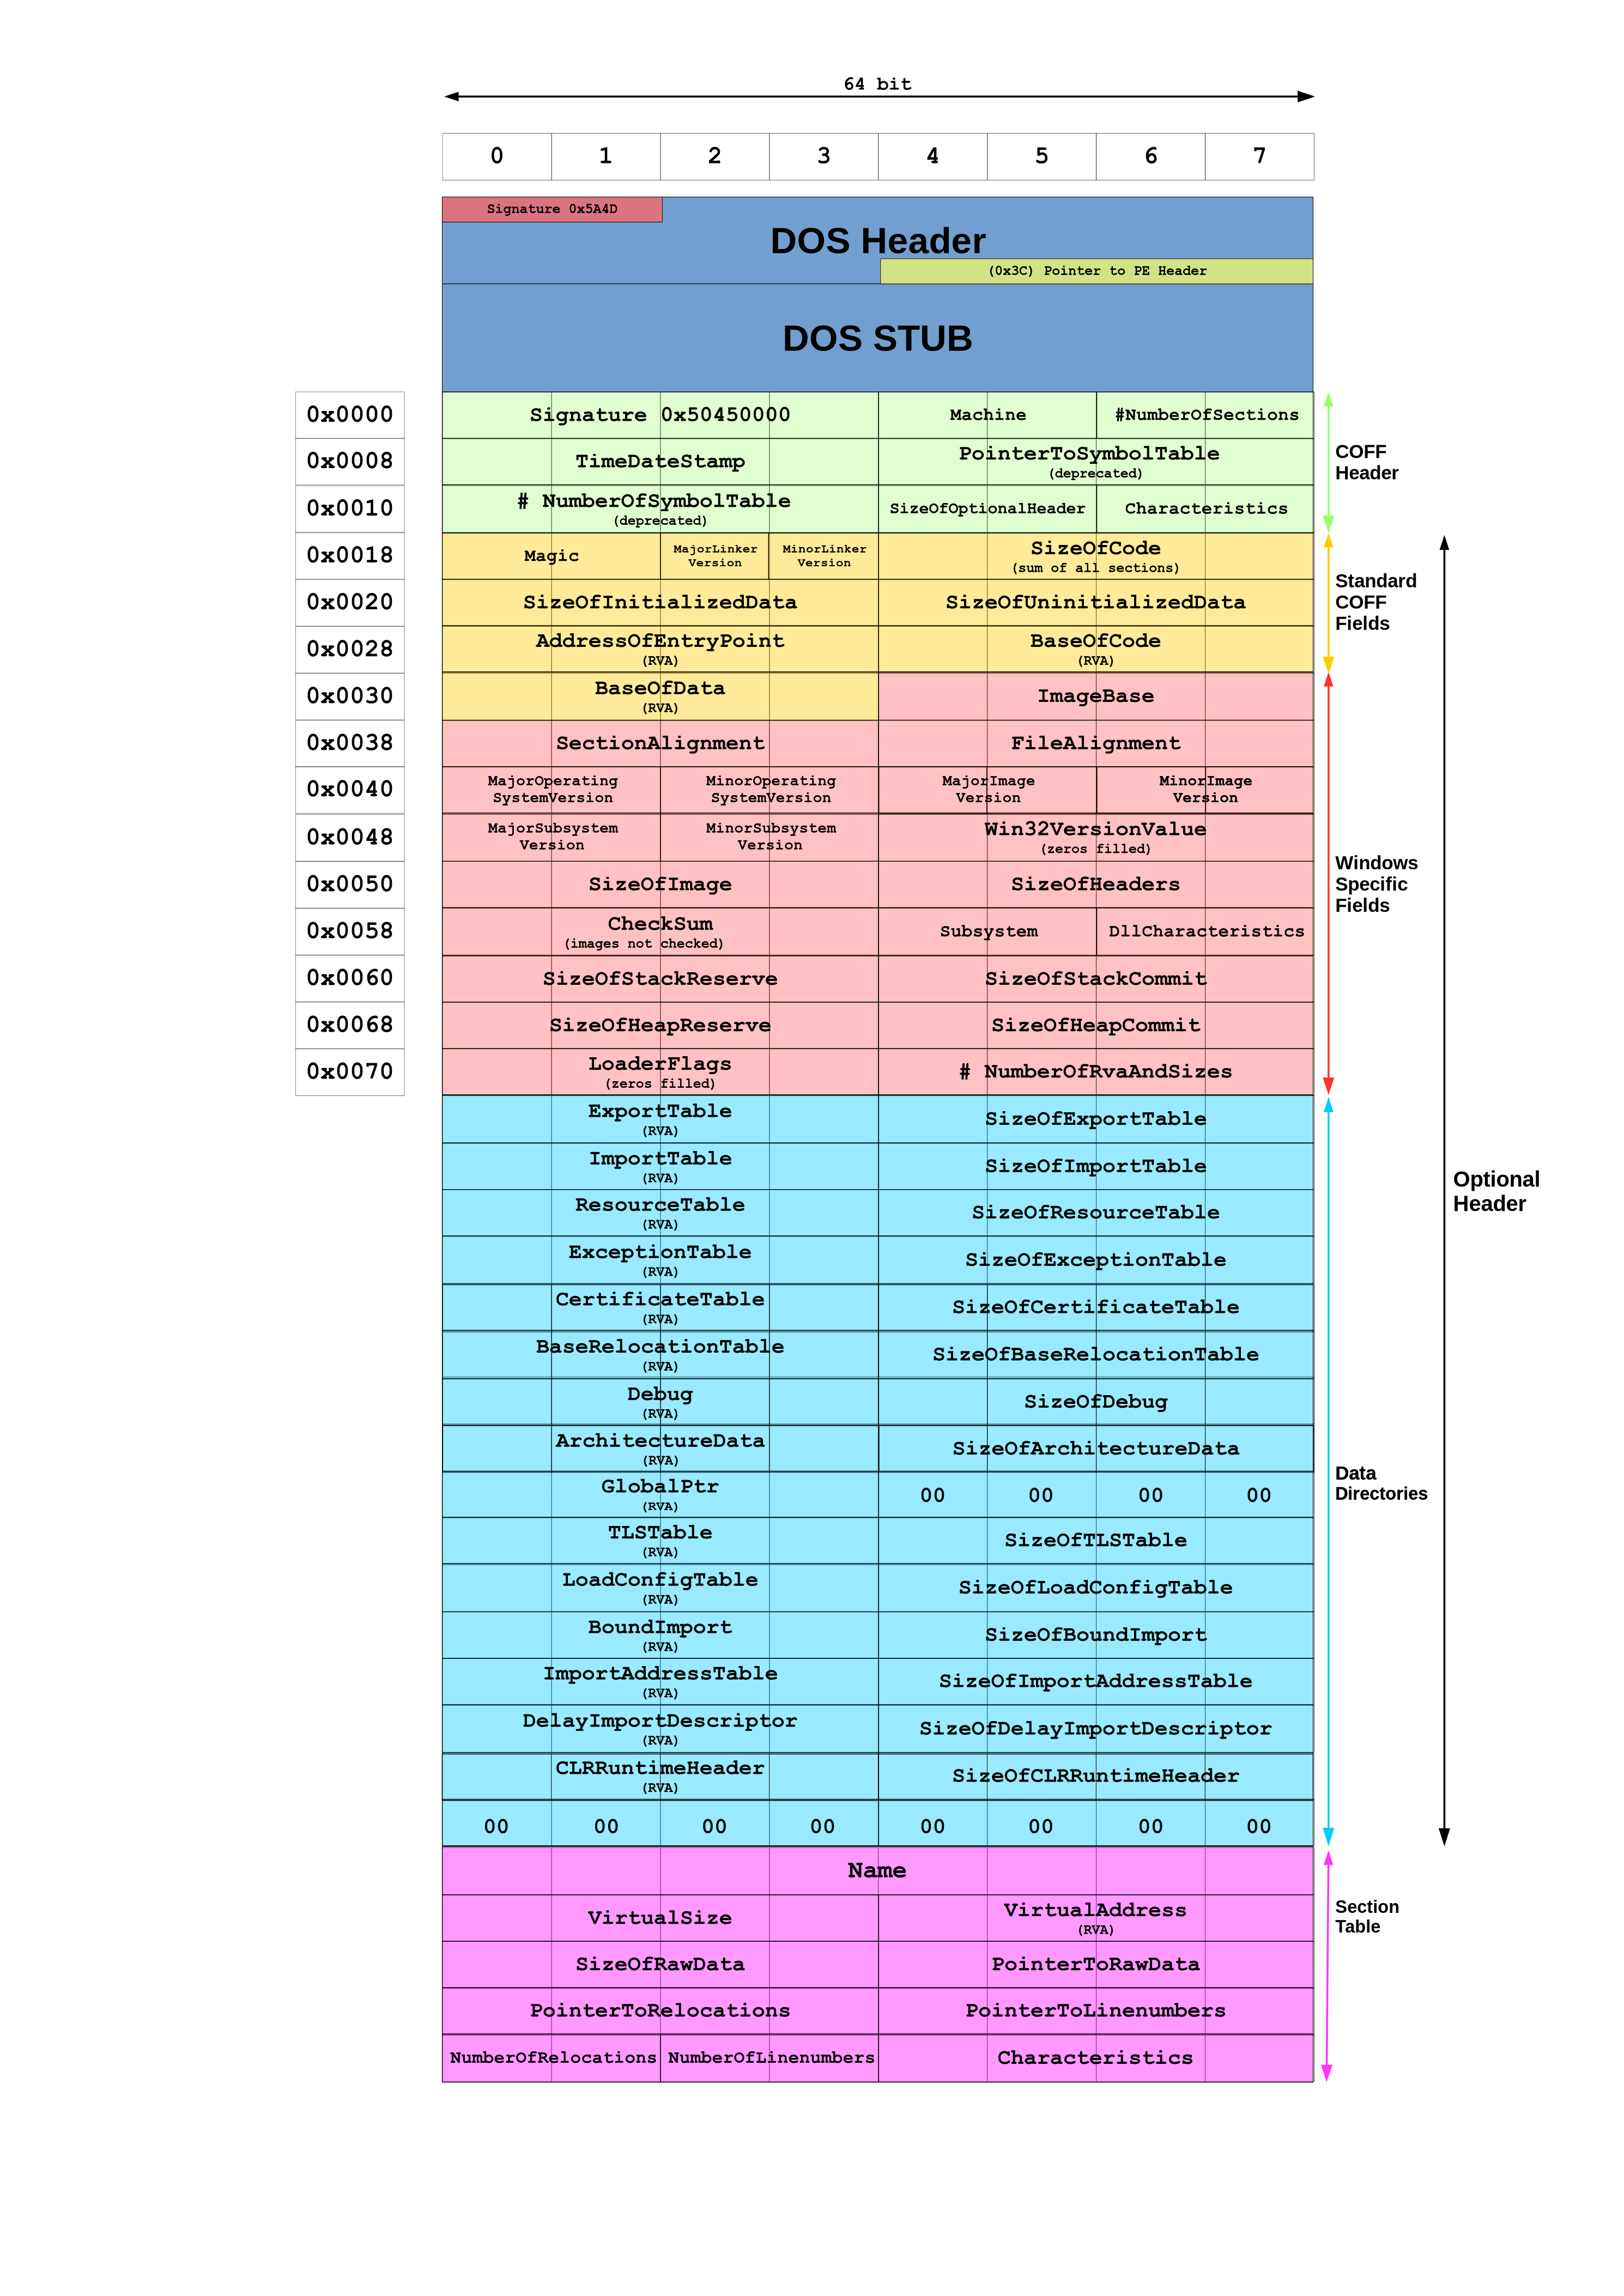
\includegraphics[width=\textwidth]{./images/Portable_Executable_32_bit_Structure.png}
	\caption{PE file structure}
	\label{fig:PEFileStructure}
\end{figure}

The PE format structure consists of a number of standard headers (\ref{fig:PEFileStructure}) followed by one or more sections and it encapsulates the information necessary for the Windows OS loader to manage the wrapped executable code: for example, among other things, it tells the dynamic linker how to map the file into memory. In particular, the PE structure usually consist of the following 3 headers:
\begin{itemize}
	\item \textit{Common Object File Format (COFF)} file header: it contains important information about the file such as the type of machine for which it is intended, its nature (DLL, EXE, OBJ), the number of sections, the number of symbols, etc.
	
	\item \textit{Optional Header}: it can be further divided into:
	\begin{itemize}
		\item \textit{Standard COFF fields}: they identify the linker version, the size of the code, the size of initialized and uninitialized data, the address of the entry point, etc.
		
		\item \textit{Windows Specific fields}: they provide windows-specific information such as minor and major operating system, subsystem and image versions, stack and heap sizes, section and file alignment, etc.
		
		\item \textit{Data Directories}: they provide pointers to the sections that follow it, which include tables for exports, imports, resources, exceptions, debug information, certificate information, and relocation tables.
	\end{itemize}
	
	\item \textit{Section Table}: it outlines the name, offset and size of each section in the PE file.
\end{itemize}

PE sections, on the other hand, contain code and initialized data that will be mapped into executable or readable/write-able memory pages, respectively, by the Windows loader at execution time, as well as imports, exports and resources defined by the file. Each section contains a header that specifies its size and address. A windows executable typically has the nine predefined sections named \textit{.text}, \textit{.bss}, \textit{.rdata}, \textit{.data}, \textit{.rsrc}, \textit{.edata}, \textit{.idata}, \textit{.pdata}, and \textit{.debug}. Some applications however do not need all of these sections, while others may define still more sections to suit their specific needs.

Among the different sections a PE file may contain here are described some of the most common:
\begin{itemize}
	\item \textit{Executable code section, \textbf{.text}}: it holds the program code. The \textit{.text} section also contains the code entry point and the \textit{Import Address Table (IAT)} (which is used as a lookup table when the application is calling a function in a different module).
	
	\item \textit{Data sections, \textbf{.bss}, \textbf{.rdata}, \textbf{.data}}: The \textit{.bss} section contains uninitialized data for the application, the \textit{.rdata} section contains read-only data. All other application/global variables are stored in the .data section.
	
	\item \textit{Resources section, \textbf{.rsrc}}: it contains resource information for a module, such as the ones required for user interfaces: cursors, fonts, bitmaps, icons, menus, etc.
	
	\item \textit{Export data section, \textbf{.edata}}: it contains export data for the application or DLL.
	
	\item \textit{Import data section, \textbf{.idata}}: it contains import data, including the import directory and import address name table.
		
	\item \textit{\textbf{.reloc} section}: it stores \textit{Relocation tables} which are used by the Windows loader to rebase the PE file if it cannot be loaded at its preferred base address. In fact, PE files normally do not contain position-independent code but are compiled to a preferred base address, and all addresses emitted by the compiler/linker are fixed ahead of time.
	
	\item \textit{\textbf{.tls} section}: it contains special thread local storage (TLS) structures for storing thread-specific local variables.
\end{itemize}

A basic PE file normally contains a \textit{.text} code section and one or more data sections (\textit{.data}, \textit{.rdata} or \textit{.bss}).

It is interesting to notice how packers sometimes create new sections, for example, the UPX packer creates a section \textit{UPX1} to store packed data and an empty section \textit{UPX0} that reserves an address range for runtime unpacking \cite{AndersonEMBER}.

\subsubsection{Feature Set Description}
EMBER feature extraction code extracts 8 groups of raw features that include both parsed features and format-agnostic histograms and string counts.

In particular, the EMBER dataset authors \cite{AndersonEMBER} made a distinction between human-readable \textit{raw features} and numerical \textit{model features} (or \textit{vectorized features}) derived from the dataset. \textit{Model features} consist of a feature matrix of fixed size used for training models, representing the numerical summary of raw features, wherein strings, imported names, exported names, etc., are captured using the feature hashing trick \cite{weinbergerFHLSML}.

\paragraph{Parsed features}
The first 5 groups of features are extracted after parsing the PE file. Anderson et al. \cite{AndersonEMBER} leveraged the \textit{Library to Instrument Executable Formats (LIEF)} \cite{LIEFProject} as a convenient PE parser. \textit{LIEF} names are used for strings that represent symbolic objects, such as characteristics and properties.

\begin{itemize}
	\item \textbf{General file information} - The set of raw features belonging to the general file information group includes the file size and basic information obtained from the PE header: the virtual size of the file, the number of imported and exported functions, whether the file has a debug section, thread local storage, resources, relocations, and the number of symbols etc.
	
	\item \textbf{Header information} - From the \textit{COFF} header, the timestamp, the target machine (string) and a list of image characteristics (list of strings) are extracted. From the optional header, instead, the EMBER feature extracting code extracts the target subsystem (string), DLL characteristics (a list of strings), the file magic as a string (e.g. "PE32"), major and minor image versions, linker versions, system versions and subsystem versions, and the code, headers and commit sizes. Then, in order to create the model features, string descriptors such as DLL characteristics, target machine, subsystem, etc. are summarized using the feature hashing trick, with 10 bins allotted for each indicator vector.
	
	\item \textbf{Imported functions} - Imported functions and libraries are extracted from the parsing of the import address table. To create numerical features, the feature vector generation code collects the set of unique library names and uses the hashing trick with 256 bins. Similarly, the hashing trick (with 1024 bins) is used to capture individual function names, by representing each as a string in the \textit{library:FunctionName} format (e.g. \textit{kernel32.dll:CreateFileMappingA}).
	
	\item \textbf{Exported functions} - The raw features include a list of the exported functions. These strings are summarized into model features using the hashing trick with 128 bins.
	
	\item \textbf{Section information} - Specific section properties are extracted from each section. They include the section name, size, entropy, virtual size, and a list of strings representing the section characteristics. Then the entry point is captured and specified by name. To convert them to model features, the hashing trick is again used on (section name, value) pairs to create vectors containing section size, section entropy, and virtual size (50 bins each). The hashing trick is also used on the entry point characteristics (list of strings).
\end{itemize}

\paragraph{Format-agnostic features}
The next 3 groups of features are instead format agnostic, meaning that they do not require the PE file to be parsed for their extraction.

\begin{itemize}
	\item \textbf{Byte histogram} - The byte histogram contains 256 integer values, representing the counts of each byte value within the file. When generating model features, this byte histogram is normalized to a distribution, since the file size is represented as a feature in the general file information.
	
	\item \textbf{Byte-entropy histogram} - The byte entropy histogram, on the other hand, approximates the joint distribution $p(H, X)$ of entropy $H$ and byte value $X$. This is done as described by Saxe et al. in \cite{saxeDNNBMDUTDBPF}, by computing the scalar entropy $H$ for a fixed-length window and pairing it with each byte occurrence within the window. This is repeated as the window slides across the input bytes. In particular, EMBER feature extraction code uses a window size of 2048 and a step size of 1024 bytes, with $16 \times 16$ bins that quantize entropy and the byte value. These counts are then normalized to sum to 1.
	
	\item \textbf{String information} - EMBER features also include simple statistics about printable strings (consisting of characters in the range \textit{0x20} to \textit{0x7f}, inclusive) that are at least five printable characters long. In particular, the code extracts information like the number of strings, their average length, a histogram of the printable characters within those strings, and the entropy of characters across all printable strings. In addition, the string feature group also provides the number of strings that begin with specific character sequences such as \textit{C:\textbackslash} (case insensitive) that may indicate a path, \textit{http://} or \textit{http://} (case insensitive) that may indicate a \textit{URL}, \textit{HKEY\_} that may indicate a registry key, etc.
\end{itemize}

\subsection{Trying to improve Dataset Loading Speed}
\color{Red}

\color{Black}
\subsubsection{Dataset Pre-Processing}
Harang et al. \cite{HarangSOREL20M} provided, together with the Sorel20M dataset, the python/pytorch code they used to load it in memory and pass it as input to their model. This code, however, is particularly I/O bounded. In fact, in order to load the data related to a single sample $i$ it first gets the corresponding sha256 hash from the Sqlite3 database (which is already loaded in memory) and then uses it as key to access the LMDB database of features. The extracted features are then decompressed and deserialized. To load the entire dataset, one batch of data of size \textit{\textbf{batch\_size}} ($=8192$ by default) is loaded at a time, repeating this process for \textit{\textbf{batch\_size}} randomly chosen samples $i$ for each batch until the end of the epoch. The code is therefore especially dependant to the hard disk random access speed. The authors of \cite{HarangSOREL20M} managed to train their model for 10 epochs in under 90 minutes, by training it on an AWS instance with high I/O speeds (exploiting a NVMe SSD), not suffering from any bottleneck. However, when using a less powerful instance not optimized for I/O performance the time needed for loading the dataset and subsequentially for training the model increased excessively. This made the use of the original data loading code for the purposes of this project unfeasible.

In order to speed up the dataset loading code the dataset is therefore pre-processed and saved in a easier (and faster) to read format. In particular the entire dataset is sequentially loaded into a set of 3 parallel memory mapped \textit{numpy} array (for the features, labels and sha256 hashes respectively) using the original data loading code after being pre-processed (the features are decompressed and deserialized), similarly to what was done in the original code every cycle. The resulting \textit{numpy} arrays are then saved 'as-is' to file. During training (or evaluation) the pre-processed dataset files are read back into memory mapped \textit{numpy} arrays 'as-is' and then used in conjunction with the default Pytorch Dataloader class, with no additional processing needed. This greatly speeded up the overall training. The main drawback of this approach is that the dataset is saved with its features being decompressed, thus taking up a much larger disk portion.

When using an instance with limited disk size the amount of space occupied by the dataset is a concern. In particular, the instance used for this project had up to 130 GB of disk space and this made it possible to train the models with only approximately half of the samples provided by Sorel20M. In fact for all the experiments only the first $6.000.000$ of the $12.699.013$ training samples, the first $1.153.846$ of $2.495.822$ validation samples and the first $1.846.154$ of $4.195.042$ test samples of Sorel20M dataset were considered. The models presented in this document therefore suffered from the smaller dataset size meaning that they cannot be directly compared with other models which used Sorel20M as base dataset. However, the code was designed to work with any dataset size so additional experimentations with more powerful instances can easily be made in the future.

\subsubsection{Generator (Dataloader) versions}
\paragraph{Pytorch Dataloader}
In the first implementation of the data loading code the original \textit{Pytorch} Dataloader class was used by passing it a specially crafted class called '\textit{Dataset}' (derived from \textit{Pytorch} 'torch.utils.data.Dataset' class) which is responsible for loading the pre-processed version of the dataset and for retrieving the data (features, labels and sha256) for a specific sample '\textit{i}'.

In particular, as it can be seen in algorithms \ref{alg:DatasetInit} and \ref{alg:DatasetGetItem}, the \textit{Dataset} class consists of 2 main member functions (although other less important member functions such as the \textit{Len} function are also implemented): \textit{Init} and \textit{GetItem}. In the \textit{Init} constructor function (alg. \ref{alg:DatasetInit}) the dataset, consisting of features (\textit{X}), labels (\textit{y}) and sha256 hashes (\textit{S}), gets loaded into a set of 3 parallel memory mapped arrays. In the \textit{GetItem} member function (alg. \ref{alg:DatasetGetItem}), instead, the data (features, labels and/or sha256) corresponding to a specific sample with index '\textit{index}' is retrieved and returned to the function caller (that will be the Pytorch original Dataloader itself).

\begin{algorithm}[h]
	\caption{Dataset class, Init}\label{alg:DatasetInit}
	\begin{algorithmic}[1]
		\Class{Dataset}
			\Function{Init}{\textit{self}, \textit{ds\_root}, \textit{mode}, \textit{n\_samples}, \textit{return\_shas}, ...}
			\State \textit{self.return\_shas} $\gets$ \textit{return\_shas}
			\State ...
			\State \textit{X\_path} $\gets$ \textit{os.}\textbf{path.join}(\textit{ds\_root}, '\textit{X\_\{\}\_\{\}.dat}'.\textbf{format}(\textit{mode}, \textit{n\_samples}))
			\State \textit{y\_path} $\gets$ \textit{os.}\textbf{path.join}(\textit{ds\_root},  '\textit{y\_\{\}\_\{\}.dat}'.\textbf{format}(\textit{mode}, \textit{n\_samples}))
			\State \textit{S\_path} $\gets$ \textit{os.}\textbf{path.join}(\textit{ds\_root},  '\textit{S\_\{\}\_\{\}.dat}'.\textbf{format}(\textit{mode}, \textit{n\_samples}))
			\State
			\State \textit{self.S} $\gets$ \textbf{load\_as\_memmap}(\textit{S\_path}, \textit{dtype}=\textbf{np.dtype}('\textit{U64}'), \textit{mode="r+"})
			\State \textit{self.y} $\gets$ \textbf{load\_as\_memmap}(\textit{y\_path}, \textit{dtype}=\textbf{np.float32}, \textit{mode="r+"})
			\State \textit{self.X} $\gets$ \textbf{load\_as\_memmap}(\textit{X\_path}, \textit{dtype}=\textbf{np.float32}, \textit{mode="r+"})		
			\EndFunction
			\algstore{bkbreak}
	\end{algorithmic}
\end{algorithm}

\begin{algorithm}[h]
	\caption{Dataset class, GetItem}\label{alg:DatasetGetItem}
	\begin{algorithmic}[1]
		\algrestore{bkbreak}
			\Function{GetItem}{\textit{self}, \textit{index}}
			\State \textit{features} $\gets$ \textit{self.X}[\textit{index}]
			\State
			\State \textit{labels} $\gets$ \{\}
			\State \textit{labels}['\textit{malware}'] $\gets$ \textit{self.y}[\textit{index}][0]
			\State \textit{labels}['\textit{count}'] $\gets$ \textit{self.y}[\textit{index}][1]
			\State \textit{labels}['\textit{tags}'] $\gets$ \textit{self.y}[\textit{index}][2:]
			\State
			\If{\textit{self.return\_shas}}
				\State \textit{sha} $\gets$ \textit{self.S}[\textit{index}]
				\State \textbf{return} \textit{sha}, \textit{features}, \textit{labels}
			\Else
				\State \textbf{return} \textit{features}, \textit{labels}
			\EndIf
			\EndFunction
		\EndClass
	\end{algorithmic}
\end{algorithm}

Before model training/evaluation the dataset generator (dataloader) is defined by passing this dataset class to the \textit{Pytorch} Dataloader implementation (\textit{torch.utils.data.Dataloader}) together with additional arguments specifying the batch size, the number of workers and whether to shuffle the data during loading (alg. \ref{alg:PytorchDataloader}). Then, during training, the \textit{Pytorch} Dataloader class will load the batches of data by iteratively calling the \textit{Dataset}'s \textit{GetItem} function \textit{batch\_size} times for each batch concatenating the extracted samples together using the \textit{torch.cat} function.

As previously mentioned, this implementation is faster than the original Sorel20M dataloader code while being also relatively simple, however given how the pre-processed dataset is saved (consecutive samples are saved on consecutive locations on disk) it is still somewhat inefficient. In fact, the time needed for completing 10 epochs training on a less powerful instance is still unreasonable. One possible optimization would be to read batches in one go as big chunks rather than calling the \textit{GetItem} function on the Dataset once per sample and then concatenating the resulting data. However, random sampling during model training introduces a regularization effect which generally improves model generalization on unseen samples, therefore it would be better to find an optimization combining both data loading efficiency and random sampling.

\begin{algorithm}
	\caption{Pytorch Dataloader definition}\label{alg:PytorchDataloader}
	\begin{algorithmic}[1]
		\State \textit{ds} $\gets$ \textbf{Dataset}(\textit{ds\_root}, \textit{mode}, \textit{n\_samples}, \textit{return\_shas}, ...)
		\State \textit{generator} $\gets$ \textbf{Pytorch\_DataLoader}(\textit{ds}, \textit{batch\_size}, \textit{shuffle}, \textit{n\_workers})
	\end{algorithmic}
\end{algorithm}

\paragraph{Generator alt1/alt2}
The first attempts at optimizing the generator were inspired by the '\textit{\textbf{index select}}' and '\textit{\textbf{shuffle in-place}}' versions of \textit{\textbf{FastTensorDataLoader}} suggested in \cite{FastTensorDataloader}.

In particular, the alternative generator 1 ('\textit{\textbf{alt1}}'), again loads the pre-processed dataset as a set of memory mapped arrays and assigns them to a set of tensors (\textit{X}, \textit{y} and \textit{S}) from which batches of data are randomly sampled using the \textit{Pytorch} '\textit{\textbf{index\_select}}' function in \textit{multithreading}.

In the alternative generator 2 ('\textit{\textbf{alt2}}'), on the other hand, the tensors created by loading the dataset as was done in \textit{\textbf{alt1}} are randomly shuffled in place at each iteration. Then the batches of data are sampled (in order) from them in \textit{multithreading}.

\begin{algorithm}
	\caption{Alt1/Alt2 FastTensorDataLoader class, Init function}\label{alg:Alt1_2FastDataLoaderInit}
	\begin{algorithmic}[1]
		\Function{Init}{\textit{self}, \textit{tensors}, \textit{batch\_size}, \textit{shuffle}, \textit{n\_workers}, ...}
		\State \textit{self.tensors} $\gets$ \textit{tensors}
		\State \textit{self.batch\_size} $\gets$ \textit{batch\_size}
		\State \textit{self.shuffle} $\gets$ \textit{shuffle}
		\State \textit{self.n\_workers} $\gets$ \textit{n\_workers}
		\State \textit{self.dataset\_len} $\gets$ \textit{tensors}[0].\textbf{shape}[0]
		\State
		\If{\textit{num\_workers} $> 1$}
		\State \textit{self.async\_results} $\gets$ [ ]
		\State \textit{self.pool} $\gets$ \textbf{ThreadPool}()
		\EndIf
		\State
		\State \textit{self.n\_batches} $\gets \lceil$\textit{self.dataset\_len} / \textit{self.batch\_size}$\rceil$
		\EndFunction
	\end{algorithmic}
\end{algorithm}

\begin{algorithm}
	\caption{Alt1 FastTensorDataLoader class, Iter function}\label{alg:Alt1FastDataLoaderIter}
	\begin{algorithmic}[1]
		\Function{Iter}{\textit{self}}
		\If{\textit{self.shuffle} $=$ \textit{true}}
		\State \textit{self.indices} $\gets$ \textbf{randperm}(\textit{self.dataset\_len})
		\Else
		\State \textit{self.indices} $\gets$ None
		\EndIf
		\State
		\State \textit{self.i} $\gets$ 0
		\State \textbf{return} \textit{self}			
		\EndFunction
	\end{algorithmic}
\end{algorithm}

\begin{algorithm}
	\caption{Alt2 FastTensorDataLoader class, Iter function}\label{alg:Alt2FastDataLoaderIter}
	\begin{algorithmic}[1]
		\Function{Iter}{\textit{self}}
		\If{\textit{self.shuffle} $=$ \textit{true}}
		\State \textit{r} $\gets$ \textbf{randperm}(\textit{self.dataset\_len})
		\For{\textit{i}, \textit{t} $\in$ \textbf{enumerate}(\textit{self.tensors})}
		\State \textit{self.tensors}[\textit{i}] $\gets$ \textit{t}[\textit{r}]
		\EndFor
		\EndIf
		\State
		\State \textit{self.i} $\gets$ 0
		\State \textbf{return} \textit{self}			
		\EndFunction
	\end{algorithmic}
\end{algorithm}

\begin{algorithm}
	\caption{Alt1/Alt2 FastTensorDataLoader class, Next function}\label{alg:Alt1_2FastDataLoaderNext}
	\begin{algorithmic}[1]
		\Function{Next}{\textit{self}}
		\If{\textit{self.i} $\ge$ \textit{self.dataset\_len}}
		\If{(\textit{self.n\_workers} $= 1$ \textbf{or} \textbf{len}(\textit{self.async\_results}) $= 0$)}
		\State \textbf{raise} \textit{StopIteration}
		\EndIf
		\EndIf
		\State
		\If{\textit{self.num\_workers} $= 1$}
		\State \textit{batch} $\gets$ \textbf{get\_batch}(\textit{self.tensors}, \textit{self.batch\_size}, \textit{self.i}, (\textit{self.indices}))
		\State \textit{self.i} $\gets$ \textit{self.i} + \textit{self.batch\_size}
		\State \textbf{return} \textit{batch}
		\Else
		\While{\textit{self.i} $<$ \textit{self.dataset\_len} \textbf{and} \textbf{len}(\textit{self.async\_results}) $<$ \textit{self.n\_workers}}
		\State \textit{arguments} $\gets$ (\textit{self.tensors}, \textit{self.batch\_size}, \textit{self.i}, (\textit{self.indices}))
		\State \textit{async\_task} $\gets$ \textit{self.pool}.\textbf{apply\_async}(\textbf{get\_batch}, \textit{arguments})
		\State \textit{self.async\_results}.\textbf{append}(\textit{async\_task})
		\State \textit{self.i} $\gets$ \textit{self.i} + \textit{self.batch\_size}
		\EndWhile
		\State
		\State \textit{current\_result} $\gets$ \textit{self.async\_results}.\textbf{pop}(0)
		\State \textbf{return} \textit{current\_result}.\textbf{get}()
		\EndIf
		\EndFunction
	\end{algorithmic}
\end{algorithm}

\begin{algorithm}
	\caption{Alt1 get\_batch function}\label{alg:Alt1GetBatch}
	\begin{algorithmic}[1]
		\Function{get\_batch}{\textit{tensors}, \textit{batch\_size}, \textit{i}, \textit{indices}, ...}
		\State \textit{batch} $\gets$ [ ]
		\If {\textit{indices} is provided}
		\State \textit{indices} $\gets$ \textit{indices}[\textit{i}:(\textit{i} + \textit{batch\_size})]
		\State
		\ForAll{\textit{t} $\in$ \textit{tensors}}
		\State \textit{batch\_data} $\gets$ \textbf{index\_select}(\textit{t}, \textit{indices})
		\State \textit{batch.}\textbf{append}(\textit{batch\_data})
		\EndFor
		\Else
		\ForAll{\textit{t} $\in$ \textit{tensors}}
		\State \textit{batch\_data} $\gets$ \textit{t}[\textit{i}:(\textit{i} + \textit{batch\_size})]
		\State \textit{batch.}\textbf{append}(\textit{batch\_data})
		\EndFor
		\EndIf
		\State
		\State \textbf{return} \textit{batch}
		\EndFunction
	\end{algorithmic}
\end{algorithm}

\begin{algorithm}
	\caption{Alt2 get\_batch function}\label{alg:Alt2GetBatch}
	\begin{algorithmic}[1]
		\Function{get\_batch}{\textit{tensors}, \textit{batch\_size}, \textit{i}, ...}
		\State \textit{batch} $\gets$ [ ]
		\ForAll{\textit{t} $\in$ \textit{tensors}}
		\State \textit{batch\_data} $\gets$ \textit{t}[\textit{i}:(\textit{i} + \textit{batch\_size})]
		\State \textit{batch}.\textbf{append}(\textit{batch\_data})
		\EndFor
		\State
		\State \textbf{return} \textit{batch}
		\EndFunction
	\end{algorithmic}
\end{algorithm}

In practice, both versions of the generator share (for the most part) the \textit{Init} and \textit{Next} functions. The main differences are, instead, in the \textit{Iter} and \textit{get\_batch} functions.

The \textit{Init} function (alg. \ref{alg:Alt1_2FastDataLoaderInit}) is used for setting up some \textit{\textbf{FastTensorDataLoader}} variables and optionally initializing the \textit{\textbf{ThreadPool}} used for \textit{multithreading}.

The \textit{Iter} function purpose is to set up the parameters for the current cycle at the beginning of each epoch. The two generator alternatives have, however, different \textit{Init} functions. In particular, generator \textit{\textbf{alt1}} \textit{Iter} function (alg. \ref{alg:Alt1FastDataLoaderIter}) resets the count of extracted samples and, if shuffling is enabled, randomly generates the current epoch sample indices (which define the order the samples are extracted from the dataset tensors). On the other hand, generator \textit{\textbf{alt2}} \textit{Iter} function (alg. \ref{alg:Alt2FastDataLoaderIter}) again resets the count of extracted samples, but if shuffling is enabled, it randomly permutes \textit{in-place} the dataset tensors themselves.

In order to get a batch of data, the \textit{Next} function (alg. \ref{alg:Alt1_2FastDataLoaderNext}), which is similar for both generator versions, is used. In particular, this function monitors the number of samples already extracted from the dataset tensors and raises a \textit{StopIteration} exception when it has cycled through all the data. Moreover, this function is also responsible for extracting and returning a batch of data from the dataset tensors. This can be done in sequence or in \textit{multithreading}. Specifically, when the number of workers selected is 1 the function sequentially gets one single batch and returns it after having updated the count of already extracted samples for the current epoch. On the other hand, if more than 1 workers are used the function prepares a number of asynchronous batch extraction tasks to be run in parallel by the threads in the thread pool, then it waits for the first result and returns it. The next call to the function will prepare other tasks and wait for the next first result. The exact number of asynchronous tasks prepared at each call is chosen dynamically to keep an array of async task results of size fixed to \textit{num\_workers} always full.

Finally, in algorithm \ref{alg:Alt1GetBatch} is shown the \textit{get\_batch} function used by generator \textit{\textbf{alt1}}: if the sample \textit{indices} are provided they are used with the \textit{index\_select} function to select the data samples for the current batch of data, otherwise a set of consecutive samples is drawn from the dataset. The \textit{get\_batch} function used by generator \textit{\textbf{alt2}} (alg. \ref{alg:Alt2GetBatch}) is simpler: it simply selects a set of consecutive samples from the dataset tensors since those were already shuffled if required.

Unfortunately, the presented two generator alternatives did not improve the data loading process enough. More specifically, when considering $6M$ samples, generator \textit{\textbf{alt1}} was only slightly faster than the original Pytorch Dataloader, while \textit{\textbf{alt2}} was even significantly slower. Generator \textit{\textbf{alt1}}, in fact, was still fairly similar to the Pytorch Dataloader implementation having used the \textit{index\_select} function instead of the slower \textit{torch.cat}. On the other hand, generator \textit{\textbf{alt2}} worked by shuffling the entire dataset tensors prior to batch extraction. If this solution surely can be more efficient for small to moderately sized dataset, it can become a bottleneck in case of huge datasets.

\paragraph{Generator alt3}
The generator alternative 3 ('\textit{\textbf{alt3}}') managed to considerably speed up the dataset loading process making a tradeoff between loading speed and samples dispersion. In fact, the time needed for 1 training epoch (considering 6M samples) passed from being of approximately 6 hours to $\sim15$ minutes.

This optimization uses a new FastTensorDataLoader class which exploits a pool of threads to asynchronously load the dataset into memory in chunks of consecutive data. In particular each thread loads into memory '\textit{\textbf{n\_chunks}}' randomly chosen chunks. Each thread then proceeds to concatenate together its '\textit{\textbf{n\_chunks}}' chunks, which contain '\textit{\textbf{chunk\_size}}' malware samples each, generating each a '\textit{\textbf{chunk\_aggregate}}', which is then randomly shuffled and returned by the thread. The \textit{\textbf{chunk\_aggregates}} are asynchronously inserted in a queue (the order depends on the threads instantiation order) of fixed length equal to the number of workers used. The main dataloader thread manages the \textit{\textbf{chunk\_aggregate}} queue, instantiating the parallel threads such that the queue is always full. Moreover, the main dataloader thread sequentially extracts, when possible, one \textit{\textbf{chunk\_aggregate}} at a time from the queue and then proceeds to return one batch of data at a time from it, when required.

\begin{algorithm} [h]
	\caption{Alt3 FastTensorDataLoader class, Init}\label{alg:Alt3FastDataLoaderInit}
	\begin{algorithmic}[1]
		\Class{FastTensorDataloader}
		\Function{Init}{\textit{self}, \textit{tensors}, \textit{batch\_size}, \textit{chunk\_size}, \textit{chunks}, \textit{shuffle}, \textit{n\_workers}, ...}
		\State \textit{self.tensors} $\gets$ \textit{tensors}
		\State \textit{self.batch\_size} $\gets$ \textit{batch\_size}
		\State \textit{self.chunk\_size} $\gets$ \textit{chunk\_size}
		\State \textit{self.chunks} $\gets$ \textit{chunks}
		\State \textit{self.shuffle} $\gets$ \textit{shuffle}
		\State \textit{self.n\_workers} $\gets$ \textit{n\_workers}
		\State \textit{self.dataset\_len} $\gets$ \textit{tensors}[0].\textit{shape}[0]
		\State
		\If{\textit{num\_workers} $> 1$}
		\State \textit{self.async\_results} $\gets$ [ ]
		\State \textit{self.pool} $\gets$ \textbf{ThreadPool}()
		\EndIf
		\State
		\State \textit{self.n\_batches} $\gets \lceil$\textit{self.dataset\_len} / \textit{self.batch\_size}$\rceil$
		\State \textit{self.n\_chunks} $\gets \lceil$\textit{self.dataset\_len} / \textit{self.chunk\_size}$\rceil$
		\State \textit{self.last\_chunk\_size} $\gets$ \textit{self.dataset\_len} $\%$ \textit{self.chunk\_size}
		\EndFunction
		\algstore{bkbreak}
	\end{algorithmic}
\end{algorithm}

\begin{algorithm}[h]
	\caption{Alt3 FastTensorDataLoader class, Iter}\label{alg:Alt3FastDataLoaderIter}
	\begin{algorithmic}[1]
		\algrestore{bkbreak}
		\Function{Iter}{\textit{self}}
		\If{\textit{self.shuffle} $=$ \textit{true}}
		\State \textit{self.chunk\_indices} $\gets$ \textbf{randperm}(\textit{self.dataset\_len})
		\Else
		\State \textit{self.chunk\_indices} $\gets$ \textbf{arange}(\textit{self.n\_chunks})
		\EndIf
		\State
		\State \textit{self.chunk\_agg} $\gets$ None
		\State \textit{self.chunk\_agg\_size} $\gets$ 0
		\State \textit{self.chunk\_i} $\gets$ 0
		\State \textbf{return} \textit{self}			
		\EndFunction
		\algstore{bkbreak}
	\end{algorithmic}
\end{algorithm}

\begin{algorithm}[h]
	\caption{Alt3 FastTensorDataLoader class, Next}\label{alg:Alt3FastDataLoaderNext}
	\begin{algorithmic}[1]
		\algrestore{bkbreak}
			\Function{Next}{\textit{self}}
				\If{\textit{self.n\_workers} $= 1$}
					\If{\textit{self.chunk\_agg} \textbf{is} None \textbf{or} \textit{self.i} $\ge$ \textit{self.chunk\_agg\_size}}
						\If{\textit{self.chunk\_i} $\ge$ \textit{self.n\_chunks}}
							\State \textbf{raise} \textit{StopIteration}
						\EndIf
						\State
						\State \textit{start\_i} $\gets$ \textit{self.chunk\_i}
						\State \textit{end\_i} $\gets$ \textit{start\_i} + \textit{self.chunks}
						\State \textit{arguments} $\gets$ (\textit{self.tensors}, \textit{self.chunk\_indices}[\textit{start\_i}:\textit{end\_i}],
						\State \hskip6.5em \textit{self.chunk\_size}, \textit{self.last\_chunk\_size},
						\State \hskip6.5em \textit{self.n\_chunks}, \textit{self.shuffle})
						\State \textit{self.chunk\_agg}, \textit{self.chunk\_agg\_size} $\gets$ \textbf{get\_chunks}(\textit{arguments})
						\State \textit{self.chunk\_i} $\gets$ \textit{end\_i}
						\State \textit{self.i} $\gets$ 0
					\EndIf
				\Else
					\While{\textit{self.chunk\_i} $<$ \textit{self.n\_chunks} \textbf{and} \textbf{len}(\textit{self.async\_results}) $<$ \textit{self.n\_workers}}
						\State \textit{start\_i} $\gets$ \textit{self.chunk\_i}
						\State \textit{end\_i} $\gets$ \textit{start\_i} + \textit{self.chunks}
						\State \textit{arguments} $\gets$ (\textit{self.tensors}, \textit{self.chunk\_indices}[\textit{start\_i}:\textit{end\_i}],
						\State \hskip6.5em \textit{self.chunk\_size}, \textit{self.last\_chunk\_size},
						\State \hskip6.5em \textit{self.n\_chunks}, \textit{self.shuffle})
						\State \textit{async\_task} $\gets$ \textit{self.pool}.\textbf{apply\_async}(\textbf{get\_chunks}, \textit{arguments})
						\State \textit{self.async\_results}.\textbf{append}(\textit{async\_task})
						\State \textit{self.chunk\_i} $\gets$ \textit{end\_i}
					\EndWhile
					\State
					\If{\textit{self.chunk\_agg} \textbf{is} None \textbf{or} \textit{self.i} $>=$ \textit{self.chunk\_agg\_size}}
						\If{\textbf{len}(\textit{self.async\_results}) $= 0$}
							\State \textbf{raise} \textit{StopIteration}
						\EndIf
						\State
						\State \textit{current\_result} $\gets$ \textit{self.async\_results}.\textbf{pop}(0)
						\State \textit{self.chunk\_agg}, \textit{self.chunk\_agg\_size} $\gets$ \textit{current\_result}.\textbf{get}()
						\State \textit{self.i} $\gets$ 0
					\EndIf
				\EndIf
				\State
				\State \textit{batch} $\gets$ \textbf{get\_batch}(\textit{self.chunk\_agg}, \textit{self.batch\_size}, \textit{self.i})
				\State \textit{self.i} $\gets$ \textit{self.i} + \textit{batch}[0].\textbf{shape}[0]
				\State \textbf{return} \textit{batch}
			\EndFunction
		\EndClass
	\end{algorithmic}
\end{algorithm}

\begin{algorithm}[h]
	\caption{Alt3 get\_chunks function}\label{alg:Alt3GetChunks}
	\begin{algorithmic}[1]
		\Function{get\_chunks}{\textit{tensors}, \textit{chunk\_indices}, \textit{chunk\_size}, \textit{last\_chunk\_size}, \textit{n\_chunks}, \textit{shuffle}}
		\If{\textit{n\_chunks} $- 1$ \textbf{in} \textit{chunk\_indices}}
		\State \textit{chunk\_agg\_size} $\gets$ (\textbf{len}(\textit{chunk\_indices}) $- 1$) $\cdot$ \textit{chunk\_size} + \textit{last\_chunk\_size}
		\Else
		\State \textit{chunk\_agg\_size} $\gets$ \textbf{len}(\textit{chunk\_indices}) $\cdot$ \textit{chunk\_size}
		\EndIf
		\State
		\State \textit{chunk\_agg} $\gets$ [ ]
		\ForAll{\textit{t} $\in$ \textit{tensors}}
		\State \textit{chunk\_agg}.\textbf{append}(\textbf{emptyTensor})
		\EndFor
		\State
		\State \textit{c\_start} $\gets$ 0
		\ForAll{\textit{idx} $\in$ [0, ..., \textbf{len}(\textit{chunk\_indices})]}
		\State \textit{t\_start} $\gets$ \textit{chunk\_indices}[\textit{idx}] $\cdot$ \textit{chunk\_size}
		\If{\textit{chunk\_indices}[\textit{idx}] $\neq$ \textit{n\_chunks} $- 1$}
		\State \textit{c\_end} $\gets$ \textit{c\_start} + \textit{chunk\_size}
		\State \textit{t\_end} $\gets$ \textit{t\_start} + \textit{chunk\_size}
		\Else
		\State \textit{c\_end} $\gets$ \textit{c\_start} + \textit{last\_chunk\_size}
		\State \textit{t\_end} $\gets$ \textit{t\_start} + \textit{last\_chunk\_size}
		\EndIf
		\State
		\For{\textit{i}, \textit{t} $\in$ \textbf{enumerate}(\textit{tensors})}
		\State \textit{chunk\_agg}[\textit{i}][\textit{c\_start}:\textit{c\_end}] $\gets$ \textit{t}[\textit{t\_start}:\textit{t\_end}]
		\EndFor
		\State \textit{c\_start} $\gets$ \textit{c\_end}
		\EndFor
		\State
		\If{\textit{shuffle}}
		\State \textit{r} $\gets$ \textbf{randperm}(\textit{chunk\_agg\_size})
		\For{\textit{i}, \textit{t} $\in$ \textbf{enumerate}(\textit{chunk\_agg})}
		\State \textit{chunk\_agg}[\textit{i}] $\gets$ \textit{t}[\textit{r}]
		\EndFor
		\EndIf
		\State
		\State \textbf{return} \textit{chunk\_agg}, \textit{chunk\_agg\_size}
		\EndFunction
	\end{algorithmic}
\end{algorithm}

More specifically, in the \textit{Init} function (alg. \ref{alg:Alt3FastDataLoaderInit}), which is similar to the \textit{Init} of the previous alternatives, some \textit{\textbf{FastTensorDataLoader}} variables are set/computed, and a \textit{\textbf{ThreadPool}} is initialized if necessary.

The \textit{Iter} function (alg. \ref{alg:Alt3FastDataLoaderIter}), instead, is used to reset the current \textit{chunk aggregate} (and its size) and the number of already processed chunks for the current cycle (or \textit{epoch}) at the beginning of each \textit{epoch}. Moreover, it also initializes the \textit{chunk indices}, which define the order in which the data chunks are retrieved, randomly or sequentially (linearly) depending on whether shuffling is required.

In algorithm \ref{alg:Alt3FastDataLoaderNext} is presented the \textit{\textbf{FastTensorDataLoader}} \textit{\textbf{alt3}} \textit{Next} member function, which is used for managing the asynchronous extraction of chunks of consecutive samples from the dataset and for returning a single batch of data. In particular, when the selected number of workers is 1 then if all the data of the current \textit{chunk aggregate} has been cycled through (or it is the first function call) the function simply extracts a single new \textit{chunk aggregate} (which is a concatenation of multiple chunks selected randomly or linearly depending on the value of \textit{self.shuffle} variable) through the \textbf{get\_chunks} function and updates the number of already processed chunks for the current \textit{epoch} and the number of extracted samples from that specific \textit{chunk aggregate}. This is however done only if the number of chunks already processed is less than the total amount of chunks, otherwise the \textit{StopIteration} exception is raised. When the number of workers is greater than 1, on the other hand, until the number of extracted chunks is less than the total amount the function prepares a number of asynchronous tasks of \textit{chunk aggregate} extraction such that the queue (of size equal to the number of selected number of workers) in which they are inserted is always full, and also updates the number of extracted chunks appropriately. Then when the current \textit{chunk aggregate} data has been explored completely (or when it is the first function call), if the async task queue is empty it raises the \textit{StopIteration} exception because it means there are no more \textit{chunk aggregates} for the current \textit{epoch}; otherwise the function gets the first async task from the queue and waits for its result (which is the extracted \textit{chunk aggregate}). Independently from the number of workers used, the function then proceeds to efficiently get a single batch of data from the current already-in-memory \textit{chunk aggregate} and returns it.

The \textbf{GetBatch} function used in generator \textit{\textbf{alt3}} is the same one already exploited in version \textit{\textbf{alt2}} (\ref{alg:Alt2GetBatch}), however, \textit{\textbf{alt3}} sees the addition of the \textbf{GetChunks} function (\ref{alg:Alt3GetChunks}) which is used to extract a number of chunks of consecutive data from the dataset and combine them into an \textit{aggregate chunk}. In particular, the function first computes the size of the resulting \textit{chunk aggregate} depending on the number of chunk indices specified and the chunk size (considering as a special case the last chunk of the dataset which may have a smaller size). Then, the \textit{chunk aggregate} itself is initialized as a series of properly sized empty tensors (one for samples features, one for labels and one for sha256 hashes) which are later filled sequentially by the data chunks got from the dataset tensors. Finally, the \textit{chunk aggregate} data gets shuffled in place, if needed, and returned.

As it can be seen from the algorithms provided, this version of the generator depends on the value a number of parameters among which the most important are \textit{\textbf{chunk\_size}} and \textit{\textbf{n\_chunks}}. Selecting different values for \textit{\textbf{chunk\_size}} and \textit{\textbf{n\_chunks}}, in fact, has an impact on the speed of the generator and on the samples dispersion. In fact the samples are not anymore randomly chosen from the whole dataset, but from a random sub-part of it (the \textit{\textbf{chunk\_aggregate}}). This effectively decreases the amount of dispersion (and randomness) of batches, possibly affecting the final model generalization. It is therefore better to consider a higher value for \textit{\textbf{n\_chunks}} possibly decreasing \textit{\textbf{chunk\_size}}. Furhtermore, the values for \textit{\textbf{chunk\_size}} and \textit{\textbf{n\_chunks}}) should be chosen in conjunction since their product results in the number of samples loaded into memory (RAM) at once for a single worker thread. Increasing too much this number (together with the number of workers used) can potentially saturate main memory (RAM) of the instance used.

\subparagraph{Generator parameters optimization}
To understand the behaviour of the FastTensorDataLoader \textit{\textbf{alt3}} on the target instance and choose the best combination of values for the parameters \textit{\textbf{chunk\_size}} and \textit{\textbf{n\_chunks}} when using 8 threads (which is double the amount of cores available in the instance used for this project), the code speed was cross evaluated on using powers of 2 for both values. In particular the data loading code was evaluated using values for \textit{\textbf{chunk\_size}} and \textit{\textbf{n\_chunks}} got from two intervals and the corresponding average \textit{speed} and average \textit{elapsed time} heatmap plots were generated.

In practice \textit{\textbf{chunk\_size}} and \textit{\textbf{n\_chunks}} values were chosen to be the powers of 2 ranging from $2^{4}$ to $2^{14}$ (included) and from $2^{3}$ to $2^{13}$, respectively. Moreover, in order to constrain the evaluation to meaningful values only, two additional parameters have to be set: \textit{\textbf{min\_mul}} and \textit{\textbf{max\_mul}}. In fact, as previously mentioned, the product of \textit{\textbf{chunk\_size}} $\times$ \textit{\textbf{n\_chunks}} gives the total number of samples in one \textit{\textbf{chunk\_aggregate}} residing in main memory; this quantity must be constrained to a certain range to avoid using too much main memory while being able to retrieve at least one \textit{batch} of data from the \textit{chunk aggregate}. The parameters \textit{\textbf{min\_mul}} and \textit{\textbf{max\_mul}} are used exactly to indicate the minimum and maximum number of batches retrievable from the resulting \textit{\textbf{chunk\_aggregates}} and therefore indirectly pose a constrain on the product \textit{\textbf{chunk\_size}} $\times$ \textit{\textbf{n\_chunks}}.

While effectively evaluating the data loading code (\textit{\textbf{alt3}}) performance the \textit{\textbf{min\_mul}} was set to a value of 1, while \textit{\textbf{max\_mul}} to 32. Those values were chosen in order to always be able to retrieve at least one \textit{batch} from the \textit{\textbf{chunk\_aggregate}} without saturating the RAM available on the instance used for this project (in fact, having for \textit{\textbf{max\_mul}} a value greater than $32 \times$ \textit{\textbf{batch\_size}} was too much).

\begin{figure}[h]
	\centering
	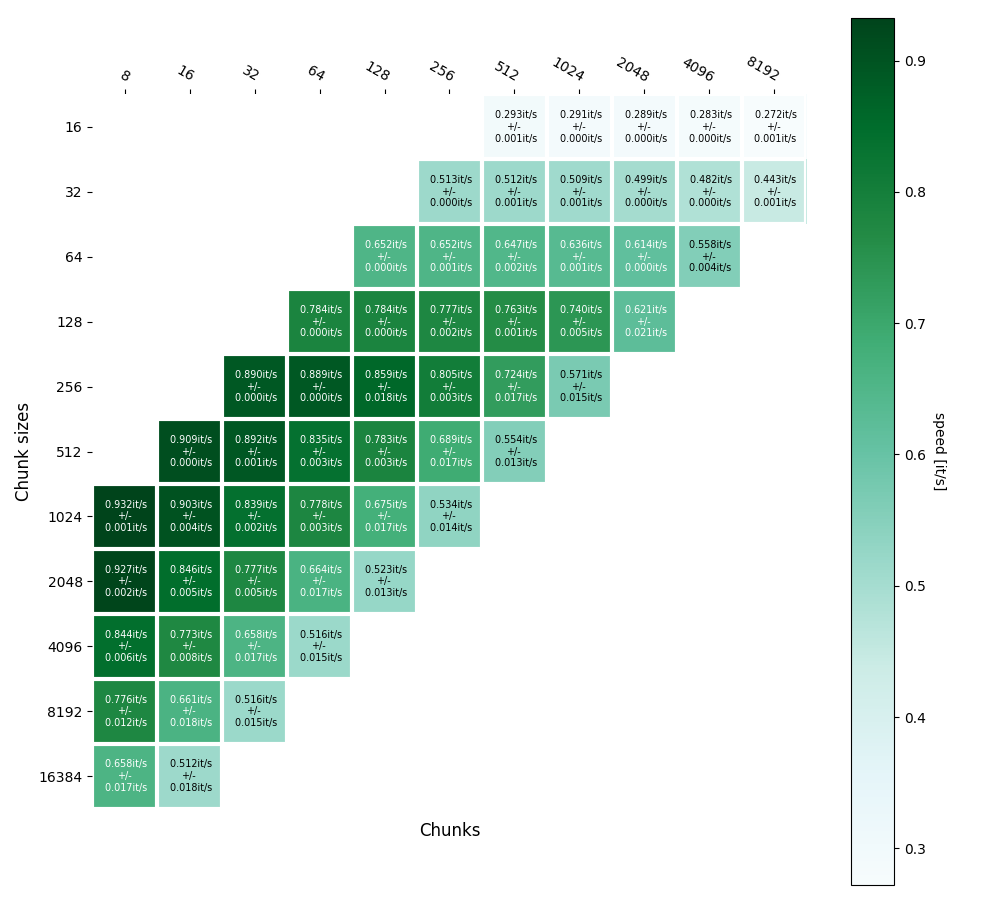
\includegraphics[width=\textwidth]{./images/speeds_heatmap.png}
	\caption{Speeds Heatmap, Higher is Better}
	\label{fig:speeds_heatmap}
\end{figure}

\begin{figure}[h]
	\centering
	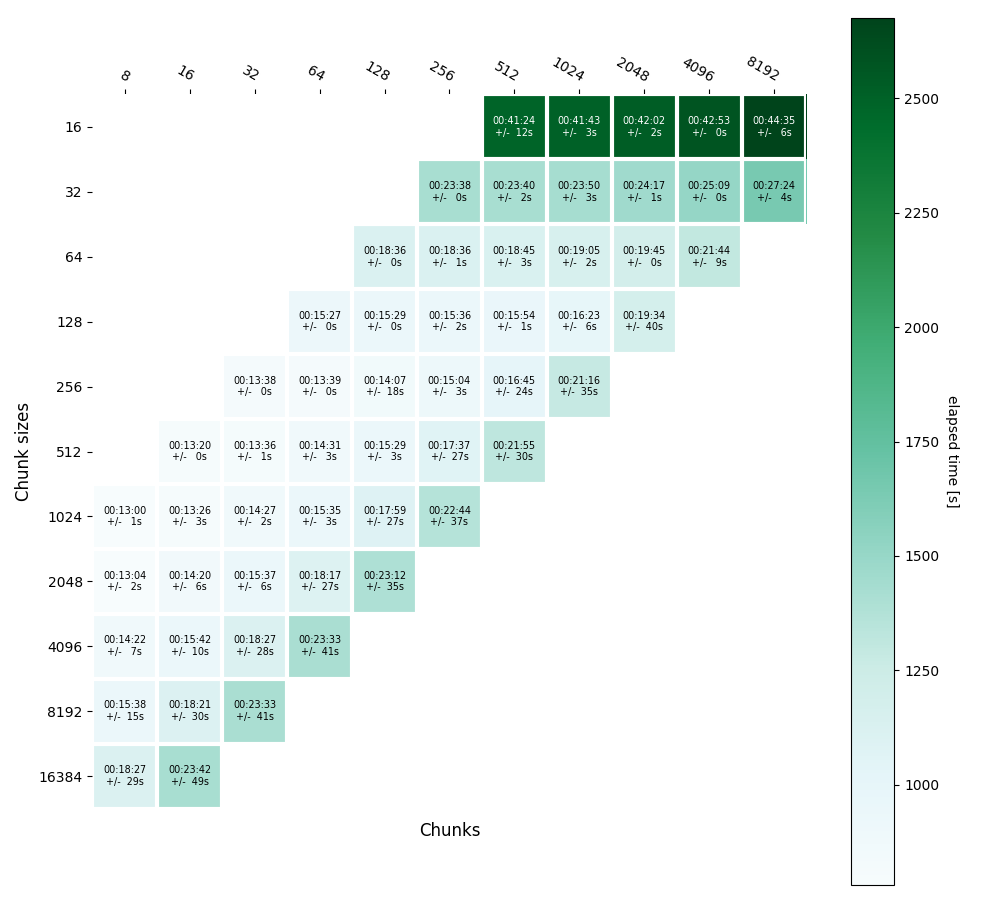
\includegraphics[width=\textwidth]{./images/times_heatmap.png}
	\caption{Elapsed Times Heatmap, Lower is Better}
	\label{fig:times_heatmap}
\end{figure}

Given the resulting heatmaps (\ref{fig:speeds_heatmap}, \ref{fig:times_heatmap}), \textit{\textbf{chunk\_size}} was permanently set to \textbf{256} and \textit{\textbf{n\_chunks}} to \textbf{256} for all the experiments conducted for this project since these values seemed to be a good compromise between data loading speed and samples dispersion.

In any case, with respect to the previous solutions (original \textit{Pytorch} dataloader and the generators \textit{\textbf{alt1}} and \textit{\textbf{alt2}}) the speed up was huge. This new version took, in fact, approximately 15 minutes, on average, to complete 1 training epoch while the previous solution took, at best, $\sim6$ hours. Therefore this was the generator used for loading the dataset in all the experiments done for this project. However, it has to be reiterated that this generator version works by approximating the random sampling step during training which in turn may hinder the model generalization on unseen samples. The results presented in this document may therefore be slightly lower than what could be achieved on a more powerful instance using the original \textit{Pytorch} dataloader.

\section{Fresh Dataset}
In order to evaluate the learned representation of PE files (embedding) of the proposed model on the sample family prediction task a further dataset, also referred to as \textit{\textbf{fresh\_dataset}} throughout this document (and in the code), was created. It consists of a number of sample files' feature vectors along with the corresponding family labels and the sha256 hashes of the original files.

More specifically, a number '\textit{\textbf{m}}' of PE malware families were selected from the list of the most prominent ones present in Italy at the time of writing (as reported by CERT-AGID summary \cite{CERTAGID}) of which Malware Bazaar provided at least '\textit{\textbf{x}}' sample files. Then, '\textit{\textbf{x}}' sample files per family were downloaded by Malware Bazaar \cite{MalwareBazaar} along with their metadata information (label, sha256 hash etc.) and the corresponding numerical feature vectors were extracted using the EMBER feature extraction and numerical feature generation codes \cite{AndersonEMBER}. Malware Bazaar, in fact, is a malware sample database maintained by malware analysts which provides examples of malware executables and high-quality manually crafted classifications/descriptions for different malware families and it is therefore a good source for creating the new (fresh) dataset.

A function called \textit{\textbf{build\_fresh\_dataset}} was specifically implemented with the purpose of creating the \textit{\textbf{fresh\_dataset}} given the following arguments:
\begin{itemize}
	\item a list of malware families (more than '\textit{\textbf{m}}') in order of importance;
	
	\item the number '\textit{\textbf{x}}' of samples per family to download;
	
	\item the number '\textit{\textbf{m}}' of families to consider.
\end{itemize}
More specifically, the function downloads '\textit{\textbf{x}}' samples per malware family from Malware Bazaar (if possible, otherwise it skips the malware family and considers the next in order of importance between the ones selected), extract the features from each sample and create the new dataset containing '\textit{\textbf{n}} $=$ \textit{\textbf{x}} $\times$ \textit{\textbf{m}}' samples which are then stored on disk as (\textit{numpy}) memory mapped array (as it was done with the pre-processed Sorel20M dataset). Therefore, between the $\ge$ \textit{\textbf{m}} malware families provided to the function, only the first \textit{\textbf{m}} for which \textit{\textbf{x}} PE samples can be retrieved from Malware Bazaar are considered.

For all the model evaluations on the \textit{\textbf{fresh dataset}} done for this project the \textit{\textbf{fresh dataset}} was composed of \textit{\textbf{x}} $= 100$ samples per family, considering the following \textit{\textbf{m}} $= 10$ families: \textit{heodo}, \textit{agenttesla}, \textit{formbook}, \textit{masslogger}, \textit{loki}, \textit{avemariarat}, \textit{njrat}, \textit{remcosrat}, \textit{netwire} and \textit{azorult}. Therefore the \textit{\textbf{fresh dataset}} consists of 1000 PE samples.

\subsection{Model Evaluation with Fresh Dataset}
The actual model representation evaluation on the \textit{\textbf{fresh dataset}} is computed by another function called \textit{\textbf{evaluate\_fresh}}. This function first randomly samples '\textit{\textbf{q}}' query samples among the ones in the $fresh\_dataset$. Then, it computes the similarity between each query sample with the other '$n-1$' samples present in the $fresh\_dataset$ ordering the latter by similarity. At this point, for each query sample there is the ranking of all the other $n-1$ samples sorted by similarity. Using those rankings the function finally calculates the \textbf{MRR} (\textit{Mean Reciprocal Rank}) and \textbf{MAP} (\textit{Mean Average Precision}) scores for the model learned representation.

The Mean Reciprocal Rank (\textbf{MRR}, \ref{eq:MRR}) is the average of the Reciprocal Ranks (\textbf{RR}, \ref{eq:RR}) of a series of queries. In particular, the Reciprocal Rank (\textbf{RR}) of a query response is the multiplicative inverse of the rank (position in the ranking) of the single sample belonging to the family of interest which classified with the highest rank (it is the closest).
\begin{equation}\label{eq:RR}
	RR(i) = \frac{1}{rank_i}
\end{equation}
\begin{equation}\label{eq:MRR}
	MRR = \frac{1} {q}\sum_{i=1}^{q} RR(i) = \frac{1} {q}\sum_{i=1}^{q} \frac{1}{rank_i}
\end{equation}
where $\textit{\textbf{rank}}_\textit{\textbf{i}}$ refers to the rank position of the first relevant sample (meaning the first sample with the same family as the current query sample) for the \textit{\textbf{i}}-th query and \textit{\textbf{q}} is the number of queries.

The \textbf{MAP} score (\ref{eq:MAP}), on the other hand, takes into account all the samples in the family of interest, with proper weights, instead of considering just the best classified one. Therefore, a model will have a higher \textbf{MRR} score if it classifies a single sample of the family of interest higher in the ranking; by contrast, it will have a higher \textbf{MAP} score if it classifies all the samples belonging to the family of interest higher in the ranking.
\begin{equation}\label{eq:PatK}
	P(k) = \frac{|\text{Relevant Samples Retrieved @} k|}{k}
\end{equation}
\begin{equation}\label{eq:AvgPatK}
	AvgP(k) = \sum_{k=1}^{n} \frac{P(k) \times rel(k)}{\text{Number of Relevant Samples}}
\end{equation}
\begin{equation}\label{eq:MAP}
	MAP = \frac{1}{q} \sum_{i=1}^{q} AvgP(i)
\end{equation}
where \textit{\textbf{P}}(\textit{\textbf{k}}) denotes the \textit{precision} at position k in the ranking, \textit{\textbf{AvgP}}(\textit{\textbf{k}}) indicates the \textit{average precision} at position k in the ranking, \textit{\textbf{n}} is the number of samples in the \textit{\textbf{fresh\_dataset}}, \textit{\textbf{rel}}(\textit{\textbf{k}}) is an indicator function which equals 1 if the sample item at rank \textit{\textbf{k}} is a relevant sample for the current query, zero otherwise, and finally \textit{\textbf{q}} is the number of queries. Moreover, a sample is considered relevant if its family is the same as the current query sample.

The \textit{\textbf{evaluate\_fresh}} provides, together with the \textbf{MRR} and \textbf{MAP} scores, the complete rankings for the $q$ query samples in a single \textit{json} file. Moreover, for convenience, 5 particular rankings are also saved as \textit{csv} files. These 5 rankings are those that produced:
\begin{itemize}
	\item the maximum \textbf{RR} (Reciprocal Rank);
	
	\item the minimum \textbf{RR} (Reciprocal Rank);
	
	\item the maximum \textbf{AP} (Average Precision);
	
	\item the minimum \textbf{AP} (Average Precision);
	
	\item the last ranking is randomly sampled between all the other rankings.
\end{itemize}

In practice, for all the experiments presented in this document the number of query samples $q$ was set to 100.

\chapter{Experimenting with ML based Malware Detection/Description methods}
\color{Red}

\color{Black}
\chapter{Proposed Tool}
\color{Red}

Description of the proposed tool..

\color{Black}
\chapter{Experiments with the proposed tool}
\color{Red}

\color{Black}
\chapter{Results}
\color{Red}

Results analysis..

\color{Black}
\chapter{Conclusions}
\color{Red}

Qui si inseriscono brevi conclusioni sul lavoro svolto, senza ripetere inutilmente il sommario.

Si possono evidenziare i punti di forza e quelli di debolezza, nonch� i possibili sviluppi futuri o attivit� da svolgere per migliorare i risultati.

\color{Black}
\chapter{Appendix}

% bibliografia scritta "a mano"
%% !TEX encoding = IsoLatin

% La bibliografia, da inserirsi solo se ci sono state citazioni.
% In questo caso ricordarsi che bisogna sempre elaborare due volte il file .TEX
% perch� la prima volta viene generata la bibliografia mentre la seconda volta viene inclusa

% NOTA: citare il DOI non � obbligatorio ma MOLTO desiderabile

\begin{thebibliography}{9} % se ci sono meno di 10 citazioni
%\begin{thebibliography}{99} % se ci sono da 10 a 99 citazioni
%\begin{thebibliography}{999} % se ci sono da 100 a 999 citazioni

% esempio citazione articolo a congresso
\bibitem{psisec}
% nomi autori
I.Enrici, M.Ancilli, A.Lioy,
% titolo articolo
``A psychological approach to information technology security'',
% nome del congresso
HSI-2010: 3rd Int. Conf. on Human System Interactions,
% luogo (stato) e data del congresso
Rzesz�w (Poland), May 13-15, 2010,
% pagine dell'articolo
pp.\ 459-466,
% DOI
\doi{10.1109/HSI.2010.5514528}

% esempio citazione articolo su rivista
\bibitem{tpa}
% autori dell'articolo
G.Cabiddu, E.Cesena, R.Sassu, D.Vernizzi, G.Ramunno, A.Lioy,
% titolo dell'articolo
``Trusted Platform Agent'',
% nome della rivista
IEEE Software,
% volume e numero della rivista (alcune riviste non ce l'hanno)
Vol.\ 28, No.\ 2,
% mese e anno di pubblicazione della rivista
March-April 2011,
% pagine dell'articolo
pp.\ 35-41,
% DOI
\doi{10.1109/MS.2010.160}


% esempio citazione capitolo di un libro fatto come collezione di contributi da autori diversi
\bibitem{tc}
A.Lioy, G.Ramunno, % autori del capitolo
``Trusted Computing'' % titolo del capitolo
nel libro % in the book
``Handbook of Information and Communication Security'' % titolo del libro
a cura di % edited by
P.Stavroulakis, M.Stamp, % nomi dei curatori
Springer, % nome editore
2010, % anno di pubblicazione
pp.\ 697-717, % pagine del capitolo
\doi{10.1007/978-3-642-04117-4_32}

 % esempio citazione pagina web di un progetto
\bibitem{openssl}
% nome del progetto
The OpenSSL project,
 % URI della pagina web
\url{http://www.openssl.org/}

% esempio citazione RFC
\bibitem{tls12}
T.Dierks, E.Rescorla,
``The Transport Layer Security (TLS) Protocol Version 1.2'',
\rfc{5246}, August 2008,
\doi{10.17487/RFC5246}

 % esempio citazione libro
\bibitem{seceng}
Ross J. Anderson,
``Security engineering'',
Wiley, 2008,
ISBN: 978-0-470-06852-6

\end{thebibliography}


% se la bibliografia � stata scritta (usando Bibtex) nel file biblio.bib allora commentare la riga precedente e scommentare le due righe seguenti
\bibliographystyle{torsec}
\bibliography{biblio}

\end{document}
